% send to DAEM
\begin{filecontents*}{example.eps}
%!PS-Adobe-3.0 EPSF-3.0
%%BoundingBox: 19 19 221 221
%%CreationDate: Mon Sep 29 1997
%%Creator: programmed by hand (JK)
%%EndComments
gsave
newpath
  20 20 moveto
  20 220 lineto
  220 220 lineto
  220 20 lineto
closepath
2 setlinewidth
gsave
  .4 setgray fill
grestore
stroke
grestore
\end{filecontents*}
%
\RequirePackage{fix-cm}
%
%\documentclass{svjour3}                     % onecolumn (standard format)
%\documentclass[smallcondensed]{svjour3}     % onecolumn (ditto)
\documentclass[smallextended]{svjour3}       % onecolumn (second format)
%\documentclass[twocolumn]{svjour3}          % twocolumn
%
\smartqed  % flush right qed marks, e.g. at end of proof
%
\usepackage{graphicx}
\usepackage{bbding}
\usepackage{graphicx}
\usepackage[cmex10]{amsmath}
\usepackage{array}
%\usepackage{mdwmath}
%\usepackage{mdwtab}
%\usepackage[caption=false,font=footnotesize]{subfig}
%\PassOptionsToPackage{hyphens}{url}\usepackage{hyperref}
\usepackage[hyphens]{url}
\usepackage{hyperref}
\usepackage{fixltx2e}

%\usepackage{multicol}
%\usepackage[titletoc]{appendix}

%\usepackage[toc,page]{appendix}

\usepackage{booktabs}
%\usepackage[capitalise]{cleveref}
\usepackage{mdwlist}
%\usepackage{multirow}
\usepackage[comma,numbers,compress,square]{natbib}
\usepackage{pgfplots}
\usepackage{placeins}
\usepackage{xspace}
%\usepackage{mdwmath}
%\usepackage{mdwtab}
%\usepackage{mathenv}
\usepackage{algpseudocode}
\usepackage{algorithm}
\usepackage{paralist}
\usepackage{wasysym}
\usepackage{comment}
\usepackage{color}
\usepackage{leading}
\usepackage{filecontents}
\usepackage{verbatim}
\usepackage{balance}
\usepackage{tikz}
\usepackage{pgf}
\usepackage{xxcolor}
\usepackage[colorinlistoftodos]{todonotes}
\usepackage{amssymb,amsmath}
\usepackage{pgfgantt}
% \usepackage{mathptmx}      % use Times fonts if available on your TeX system
%
% insert here the call for the packages your document requires
%\usepackage{latexsym}
% etc.
%
% please place your own definitions here and don't use \def but
% \newcommand{}{}
%
% Insert the name of "your journal" with
% \journalname{myjournal}
%
\begin{document}

\title{A PROBABILISTICALLY ANALYZABLE CACHE TO ESTIMATE TIMING BOUNDS%\thanks{Grants or other notes
%about the article that should go on the front page should be
%placed here. General acknowledgments should be placed at the end of the article.}
}
%\subtitle{Do you have a subtitle?\\ If so, write it here}

%\titlerunning{Short form of title}        % if too long for running head

\author{Hassan Anwar        \and Chao Chen
        \and Giovanni Beltrame %etc.
}

%\authorrunning{Short form of author list} % if too long for running head

\institute{H. Anwar \at
              Polytechnique Montr\'eal \\
              Tel.: +01-514-992-3394\\
              %Fax: +123-45-678910\\
              \email{hassanbinanwar@gmailcom}           %  \\
%             \emph{Present address:} of F. Author  %  if needed
       %    \and
        %   S. Author \at
          %    second address
}

\date{Received: date / Accepted: date}
% The correct dates will be entered by the editor


\maketitle

\begin{abstract}
Modern computer architectures are targeted towards speeding up
  the average performance of software running on it. Architectural
  features like: deep pipelines, branch prediction, out-of-order
  execution, and multi-level memory hierarchies have an adverse impact on software timing prediction. Particularly,
  it is hard or even impossible to make an accurate estimation of
  the worst case execution-time (WCET) of a program or software running on a particular hardware platform. 
 

Critical real-time embedded systems (CRTESs), e.g. computing systems
  in aerospace require strict timing constraints to guarantee their proper operational behavior. WCET analysis is the central idea of
  the real-time systems development because real-time systems always need to meet their deadlines. In order to  meet the deadline requirements, WCET of the real-time systems tasks must be determined, and this is only possible  if the hardware architecture is time-predictable. Due to the unpredictable nature of the modern computing hardware, it is not practical to use advanced computing systems in CRTESs. The real-time systems do not need to meet high-performance requirements. The processor designed to improve average cases performance may not fit the requirements for the real-time systems due to predictability issues.
  


  Current timing analysis techniques are well established, but require
  detailed knowledge of the internal operations and the state of the
  system for both hardware and software. Lack of in-depth knowledge of
  the architectural operations become an obstacle for adopting the 
  deterministic timing analysis (DTA) techniques for WCET measurement.
  Probabilistic timing analysis (PTA) is a technique that emerged for the timing analysis of the next-generation real-time systems. The PTA techniques reduce the extent of knowledge of a software execution platform that is needed to perform the accurate
  WCET estimations.
In this thesis, we propose the development of a new probabilistically  analyzable cache and applied
PTA techniques for time-prediction. In this work, we implemented a randomized cache for MIPS-32 and Leon-3 processors. We designed and implemented random placement and replacement policies, and applied probabilistic timing techniques to measure probabilistic WCET (pWCET). We also measured the level of pessimism incurred by the probabilistic techniques and compared it with the deterministic cache configuration. The WCET prediction provided by the PTA techniques is closer to the real execution-time of the program. We compared the estimates with the measurements done
 on the processor to help the designer to
 evaluate the  level of pessimism introduced by the cache architecture
 for each probabilistic timing analysis technique.
 This work makes a first attempt towards the comparison of
 deterministic, static, and measurement-based probabilistic timing
 analysis for time-prediction under varying cache configurations. We identify  strengths and limitations of each technique for time- prediction, and provide guidelines for the design of the processor that minimize the pessimism associated with WCET. Our experiments show that the cache fulfills all the requirements for PTA and program prediction can be determined with arbitrary accuracy. Such probabilistic computer architecture carries unmatched potential and great
  promise for next generation CRTESs.   












\keywords{WCET \and PTA \and SPTA \and MBPTA \and FPGA \and Timing Analysis}
% \PACS{PACS code1 \and PACS code2 \and more}
% \subclass{MSC code1 \and MSC code2 \and more}
\end{abstract}

\section{Introduction}
\label{intro}
Time-prediction is the key requirement of a critical real-time embedded system (CRTESs)~\cite{Cazorla:2013:PPA:2465787.2465796}. The next generation of real-time systems will heavily depend on the accurate prediction of worst-case execution-time (WCET) of software running on a particular processor. Current processor architectures are based on the following paradigm: \textit{Make the common case fast and the uncommon case correct}~\cite{Schoeberl:2009:TCA:1540555.1554265}. This design approach leads towards architectures in which the average-case execution-time is optimized at the cost of worst-case execution-time. Modelling the performance enhancement features of current processors, e.g. pipelining, multi-level cache, dynamic branch prediction, out-of-order execution, chip-multi-threading, and speculative execution for WCET analysis often results in computationally infeasible problems. Real-time systems need an architecture in which the most primary design parameters are a fast and predictable worst case. The work accomplished in this project is focused on the design and usage of probabilistically analyzable cache for time-prediction. The measurements of probabilistic worst-case execution-time bounds (pWCET) under varying randomized cache configurations are the central idea. The time-prediction analysis is performed by using probabilistic timing analysis (PTA) techniques.
Drawing our inspiration from~\cite{Cazorla:2013:PPA:2465787.2465796}, we implement the probabilistically analyzable time-predictable cache which can be used to apply PTA techniques. The idea stems from the research on real-time systems and the fact that these systems have to be used in a real-time  environment, e.g. air-bag system in a car, auto-braking system on a plane, etc. All these systems should be timeliness; this means missing a deadline could have serious repercussions. Knowing the upper bound of the system execution-time allows the experts to design their systems in a way that keeps the worst execution-time in content.

WCET estimation of a probabilistically analyzable system can be determined through static probabilistic timing analysis (SPTA)~\cite{Griffin:2014:SPT:2659787.2659809} and measurement-based timing analysis (MBPTA)~\cite{cucu2012measurement} techniques. Both techniques provide cumulative distribution function or pWCET function that upper bounds the execution-time of a program. The analysis guarantees that the execution-time of a program only exceeds the corresponding execution-time bound with the probability lower than a targeted probability. In this project, we will explore both static and measurement-based probabilistic timing techniques. 


Static probabilistic timing analysis is based on an extension of a real-time calculus~\cite {Santinelli:2011:TPR:1967021.1967028} while measurement-based probabilistic timing analysis is based on measurements of the execution-time at a higher level of abstraction. The methodology uses in this work will leverage the probabilistic approach to solve the dependability problem of the program on the execution history. The dependability problem can be solved by introducing the randomization in the hardware components, e.g. randomized placement and replacement cache policies. Due to randomization, we implement a probabilistic system which follows a particular mathematical property that is essential to be able to apply PTA techniques --- \textit{the execution-time behavior of the system is independent and identically distributed}~\cite{gumbel1954statistical}.  
The SPTA and MBPTA have been commonly used for pWCET estimations for real-time systems. These timing techniques are used for real-time systems since probabilistic techniques do not dependent on any history~\cite{Kosmidis:2013:CDP:2485288.2485416}. 
% 

Probabilistic analysis of a cache has been an active research field in the last couple of year~\cite{Kosmidis:2013:CDP:2485288.2485416, Jalle:2014:BDT:2616606.2616668}. Most of the work presented so far is based on simulation or development of the timing techniques. The application of PTA techniques on timing measurements extracted from the probabilistically analyzable hardware has not been extensively explored. Furthermore, the probabilistic analysis of the hardware processor such as processors implemented on FPGA~\cite{ION, leon3} is not studied so far. Therefore, the probabilistic analysis of the computing system is of great interest for the real-time systems community. In this work, we used open source VHDL cores of MIPS-32 and Leon-3 and integrated randomized cache in it. 




\subsection{Context and Motivation}

In general, determining the WCET bound on a hardware platform is a challenging task due to the complexity of the processor architectural design. The unavailability of the proprietary processor designs makes it more complicated. Accurate modelling of the design for a worst-case execution-time calculation is a tedious job. Moreover, as discussed earlier, features that enhance average performance heavily depend on the execution history, e.g. memory traces of the instructions. The history is hard to model for WCET analysis since a long history leads towards the state explosion problem for the final WCET. The probabilistic timing analysis is an emerging technique which helps eliminate the need for the detailed design knowledge and execution history required to model the timing behavior of all the architectural components.

To enable the probabilistic timing analysis of the applications running on a processor, we need to introduce randomization in the timing behavior. The randomization in timing is achieved by employing  randomized placement and replacement policies for L1-cache.  The randomization helps to make the system more predictable, i.e. if the probabilistic response of the system is known, meaningful predictions can be made using the arbitrarily specified confidence interval. The prediction comes with pessimism due to the overestimation generated by the timing analysis techniques~\cite{Cazorla:2013:PPA:2465787.2465796}. Therefore, we need a new constructive approach for designing processor architectures to minimize this pessimism. For this purpose, processors need to consider time predictability as a major and important factor in their design. In other words, an architecture design with a new paradigm based on \textit{Make the worst case fast and the whole system easy to analyze}~\cite{Schoeberl:2009:TCA:1540555.1554265}. General-purpose processors are designed to maximize throughput~\cite{Cazorla:2013:PPA:2465787.2465796}. Real-time systems require a processor in which WCET is reasonable and known at design time. Classical performance enhancement techniques in computer architectures are extremely hard to model for the WCET analysis. For example, execution history is considered as key for performance improvements, but also the main issue for WCET analysis. Therefore, we need different techniques to manage execution history. The processors designed for low WCET will never be as fast as the processors designed for performance improvement. There are two different design methodologies; either to design for an accurate WCET analysis or for fast computations.
Therefore, deterministic computer architecture provides WCET bound that is higher than the real WCET in which the level of pessimism is very high. The difference between the real WCET and the bound is caused by the pessimism of the analysis due to certain factors such as  infeasible execution path, lack of certain information, complex architectural design, lack of information provided by the vendors, and state explosion problem due to long execution history.  Here, we would like to present our idea of the probabilistically analyzable cache. 
 
Timing analysis for probabilistic architecture can be performed by using probabilistic timing analysis techniques which provide probabilistic WCET bounds (\small{p}WCET)~\cite{Cazorla:2013:PPA:2465787.2465796}. WCET bounds derived from probabilistically analyzable computer architecture is almost equal to the real WCET. 
To design a probabilistic analyzable system, we used randomized cache~\cite{anwar2015probabilistically}. 
%to achieve the minimum dependency on the execution history. We will not only restrict the features of the current processors (e.g. pipelining, cache, branch prediction, instructional level parallelism, and chip-multi-threading). But, also, add features which will help to enhance performance and time predictability.
 We will use two variants of PTA, i.e. SPTA~\cite{Altmeyer:2015:SPT:2726097.2726149} and MBPTA~\cite{cucu2012measurement}.
In this context, we design and implement the probabilistically analyzable time predictable cache to improve timing analysis bounds.
% 
\subsection{Objectives/Purpose of Study}
The objective of this research is the definition and implementation of a fully probabilistically analyzable cache for time-prediction. In this research project, we design and implement the probabilistic cache to perform probabilistic timing analysis on the timing values derived by running the benchmark (C-codes) on the processor. The PTA techniques are developed as a solution to reduce the amount of information needed to determine tight WCET estimates. Probabilistic analysis estimates the chance of forthcoming actions based on an a priori model of the probability. It is a novel approach to timing analysis of next-generation real-time embedded systems. The observed execution-times of programs having the distinct probability of occurrence  can be modelled with independent and identically distributed random variables. Current processors do not fulfil these properties due to their deterministic nature. To guarantee a particular probabilistic timing behavior of a system, we have to remove determinism from computer architecture because determinism introduces dependencies between instructions and it is not possible to make any assumptions of a normal distribution of events. Our approach is to guarantee the randomness and normal distribution of events inside all hardware components using a real random number generator~\cite{Matsumoto:1998:MTE:272991.272995}. The purpose of this project is to make possible the probabilistic timing behavior at the hardware level. The project includes the development of a hardware infrastructure aimed at design space exploration for future power-efficient and high-performance computer architectures for real-time embedded systems which include randomized caches. The hardware implementation of the probabilistic cache will be the main goal.
% We will develop %the hardware architecture for a stochastic processor which leads towards the development of the %instruction processor design and memory interface and try to establish, improve techniques to %cumbersome timing issues by not only improve the results of the older techniques but also propose %our own novel ideas and techniques for probabilistic computer architecture.
We used benchmarks with high industrial relevance. The pessimism observed under different cache configurations with PTA techniques on the probabilistic architecture is also studied.

\subsection{Problem Statement}
This thesis aims at defining a novel approach for probabilistically analyzable cache for the real-time systems. In particular, our work intends to provide solutions able to mitigate multiple problems, including, but not limited to:

\begin{itemize}

\item{Randomization in the timing behavior of the hardware components (e.g. randomized cache) to make the system more predictable. If the probabilistic response of the system is known, meaningful predictions can be made using arbitrarily specified confidence intervals}.

\item{Cache plays an important role for performance enhancement. Therefore, we design a randomized cache that is organized to speed-up execution-time and provide tight WCET bounds}.
\item{Utilization of both variants of PTA techniques to understand and study how PTA techniques affect the prediction bound}.
\item{To implement the effective probabilistic analyzable cache, one has to consider (a) time-prediction as the first order design parameter (b) the design should be probabilistically analyzable and can be used to define the bound for pWCET, and (c) feasible for real-time systems. The purpose is the definition of a probabilistically analyzable system that can work under real-time constraints and it is sufficiently fast to meet performance requirements}.
 
 %\item The occurrence of transient and permanent faults in aerospace systems need to be detected, classified, and mitigate for timing analysis %\item Demonstrate the technology with CubeSat platform \end{itemize}.
\end{itemize}

The main challenges we foresee are: 
\begin{itemize} 
\item{Finding the architectural issues and their solutions}.
 \item{Designing novel timing analysis techniques and their validation and evaluation}.
 \item{Implementing a randomized cache and integration with the processors}.


\end{itemize} 

These challenges are addressed by using probabilistic techniques, such as SPTA and MBPTA, and by improving existing timing analysis techniques (e.g. the work done in~\cite{Altmeyer:2015:SPT:2726097.2726149} used random replacement cache for timing improvement) or by introducing a novel technique. We implement the  architecture, i.e. processor with probabilistic cache as a prototype system  is implemented on an field-programmable gate array (FPGA). 
Its effectiveness is evaluated by making use of  benchmark suites such as the M{\"a}lardalen benchmark~\cite{mrtc:bench}. 
For the system implementation, we use existing tools, i.e.  Gaisler LEON3~\cite{leon3} processor, and ~\cite{ION} and modify it accordingly to meet our needs. We studied pessimism and time- prediction under varying  cache parameters, such as cache-line, cache-size, and associativity.

\subsection{Novelty and Impact}
The main contributions of this research project can be summarized as follows:

\begin{itemize}

\item{Development of  the probabilistic component --- randomized cache.  The randomization is based on a parametric hash function and can be extended to implement other probabilistic components, e.g. probabilistic bus}.
\item{Development of a methodology of timing analysis for the probabilistic systems. The probabilistic properties can be realized by using caches with random placement and replacement policies}.
\item{Investigation of prediction effects for probabilistic systems under varying cache configurations. The techniques to predict timing analysis bound for estimation ensure the reliability of real-time systems.
Moreover, with successful probabilistic cache implementation and its analysis, it can bring enormous benefits for software production, verification, and certification cost. The aerospace industry of Quebec and Canada, as well as other technology areas, will benefit from knowledge transfer and commercialization of probabilistic real-time system software development}.
\end{itemize}

\subsection{Timing Analysis}
\label{sec:1}
This chapter discusses the related work in Timing Analysis (TA) techniques, which have two variants --- deterministic and probabilistic. We discuss how these two techniques have been used in the past to estimate WCET bound. TA techniques have significant value in real-time systems to determine the WCET bound and henceforth ensure the accurate behavior of the system. The good knowledge of a timing analysis is the key to designing CRTESs.

The family of timing analysis techniques can be classified into two sub-categories: deterministic timing analysis (DTA), and probabilistic timing analysis (PTA)~\cite{mezzetti2015randomized}. Furthermore, the TA techniques can be classified into four distinct approaches: static and measurement-based deterministic timing analysis (SDTA and MBDTA) and static and measurement-based probabilistic timing analysis (SPTA and MBPTA)~\cite{mezzetti2015randomized}. The main purpose of timing analysis is to calculate the tight bounds of WCET.



\subsection{Deterministic Timing Analysis Techniques} 


%derive,derived = obtain, get take
Finding the WCET of a program consists of three possibilities (a) computing the execution-times of all possible execution paths (b) computing the execution-times of a set of possible paths that can be guaranteed to include the longest path and (c) computing the execution-time of the longest possible path.  To perform any of these three methods, two approaches can be considered (a) deterministic timing analysis based on the model of the hardware and software code representation (b) execution of the program code on the real hardware (measurement-based approach).
 
Firstly, deterministic timing analysis techniques are discussed. These are considered as the classical  techniques used to find WCET bound~\cite{wilhelm2005determining}. These techniques consider time taken by the task or program depending on the time spent in instructions, a particular path, and specific hardware~\cite{wilhelm2008worst}. This technique requires modelling of the architecture and building a representation of the program, e.g. syntax tree that represents the structure of the code. Control flow graph is also used to express the structure of the executable code. To calculate the execution-time bounds for timing analysis problems, this technique splits the task into a sequence of sub-tasks. These sub-tasks deal with the properties of the control flow and others with the execution-time of instructions/series of instructions on a particular hardware. The timing methods provide the execution-time bound with the guarantee that the execution-time of the program will not exceed the derived bounds. The attempts to find the execution-time bounds analyze the possible control-flow paths and the execution-times for this set of paths. 
There are two approaches for deterministic timing analysis techniques named static techniques and measurement-based techniques.



\subsection{Static Techniques}


Static techniques are used to estimate WCET by examining the source code without executing it on the hardware. Researchers started developing static techniques for industry in the late 1980s. However, the most popular industrial standards are \textit{end-to-end timing measurements techniques}. A lot of work has been done for static timing techniques. Static techniques work at a higher-level of abstraction to determine the structure of a program's task and subtask. It works on either a piece of the source code or disassembled binary executable. This technique also works at a low-level using timing information about the real hardware on which the code will eventually run, considering this information as a representation of the hardware. The model needs to consider all aspects of the hardware such as pipeline, branch prediction, and cache. However, obtaining execution-times from a model instead of measuring it on a hardware platform is only possible if a realistic model of the architecture is available. After combining high and low level techniques, the tool attempts to give an upper bound on the execution-time required to execute a particular code on a hardware platform~\cite{wilhelm2008worst}. At the low-level, static techniques use the behavior of architectural features that improve the average-case performance of the processor, e.g. instruction/data caches, branch prediction and instruction pipelines. It is likely, but increasingly complex, to determine tight WCET bounds if the advanced architectural features are taken into account in the timing model. For example, cache locking techniques can be used for analyzing WCET estimation but provide predictability far away from the actual execution~\cite{bernat2002wcet}. This is one of the reasons the research community is shifting towards probabilistic techniques which we discuss in section~\ref{PTAT}. Static techniques give good results for simple hardware. Hence, a possible limitation of the static technique is the hardware (the processor architecture itself) because the processor hardware has reached a level complexity that it is very hard to model. The modelling process can introduce errors from several sources like chip design errors, lack of documentation (companies do not provide the detail of the architecture), errors in model creation, etc. As a result, the developed model predicts a different behavior to that observed on real hardware with more pessimistic bounds than the actual ones. Typically, when it is impossible to have accurate predictions, a pessimistic result is used. Modelling a multi-core processor for WCET estimations is even harder than single-core processor. There are many popular and academic tools that implement various forms of static techniques such as aiT, Rapitime, and Bount-~\cite{wilhelm2008worst}.


%
%
%\item {The static techniques are not based on the code execution  on the hardware platform rather than take the task code itself combine it with 
%some annotations, analyze the set of possible control flow paths through the task, combine control flow with some  model of the hardware architecture, and obtain upper bounds for this combination~\cite{wilhelm2008worst}}.

\subsection{Measurement Techniques}
\label{MBT}

The measurements techniques get the timing information by executing the task on the hardware with a given set of inputs. No modelling and assumptions are required for this technique~\cite{wilhelm2008worst}. This technique measures the maximum/minimum observed execution-time, or execution-time distribution. Measurement-based timing techniques usually measure the execution-times of the tasks on the real hardware to produce an estimate of the WCET bound. This technique is used to find the execution-times either on all execution paths, or on a subset of execution paths. Finding execution-times of all possible paths does not guarantee the WCET since the longest path may be missed. One approach is to divide the task into sub-tasks and find the WCET for each sub-tasks. Then, it is easy to combine it with the high-level analysis to get the WCET estimates. The small sub-tasks of the primary task can be measured automatically using techniques such as instrumentation (adding markers to the sub-tasks) or with hardware support such as debuggers and processor hardware tracing modules. These markers help to find the traces of the execution-times which involve both the path taken by the task and the time at which different points are executed. The trace is then analyzed to find the maximum time that each part of the sub-tasks used. Measurement-based timing analysis provides less pessimistic results for complex hardware~\cite{kosmidis2014measurement}. This technique is different from the static analysis which suffers from extreme pessimism. Therefore, measurement-based techniques are the industrial standard with some limitations, i.e. it relies on observing the worst-case measured execution-time during the testing, and it is hard to execute it for all the test cases that  might affect the worst-case. There are few tools available in the market to measure the execution-time bound by using measurement timing techniques. Among those, the most famous are Chalmers, SWEET and Heptane~\cite{wilhelm2008worst}.


\subsection{Comparison Between Static and Measurement Techniques}

In this section, we compare the static and measurement-based techniques to highlight the differences and similarities in their execution-time methodologies, abilities, and technical problems. Static methods are based on control-flow analysis and bound calculation to cover all possible execution paths and estimate the WCET. The overestimation is due to the processor-specific modelling. The main advantage of static methods is the fact that the analysis can be done without
running the program on an actual hardware. This analysis method often needs high-tech equipment to simulate the hardware and peripherals of the targeted system. 

Measurement-based methods use real measurements (execution runs). Except for the case in which all potential execution paths are measured or the processor is simple enough to let each measurement be started in a worst-case initial state, there is still a chance that some context-dependent execution-times may be missed. For this reason, this  method is unsafe to some extent. To calculate estimations, the measurement methods may use control-flow analysis to include all possible execution paths or they may only use the observed execution paths. The benefit of using  measurement-based technique is that it is simpler to apply because it requires no need to model processor behavior and it produces WCET and best case execution-time estimates. The results are more precise, closer to the exact WCET bounds and also incurs less pessimism as compared to the static techniques especially for complex processors. 
Both techniques share some technical problems and solutions. The front-ends are similar as both use: a) executable code as input b) control-flow analysis c) bound/estimate prediction can be similar. For example, the implicit path enumeration technique (IPET)~\cite{abella2014comparison} used for prediction is employed by some static tools and by some measurement-based tools~\cite{kosmidis2014pub}.
The main technical problem for static techniques is the modelling of processor behavior which is not an issue for most measurement-based technique, for which the main issue is to measure the execution-times accurately with fine granularity. The handling of the timing anomalies gives an interesting comparison of both the techniques.
Timing anomalies are hard to access for the measurement-based technique that makes it very hard to find a
worst-case initial state. To remain on  the safe side, the measurement should
 be done for all possible initial states, which is unrealistic. 
Measurement-based techniques use only a subset of initial states.
Static techniques are based on an abstract interpretation. Therefore, static techniques have ways to express the absence
of information and analyze large state sets including all possible
states for a safe analysis. 


\subsection{Probabilistic Timing Analysis Techniques}
\label{PTAT}
%\section{Timing Analysis}
As discussed in section~\ref{sec:intro}, advancement in the architectural features, adoption of more complex systems lead towards the \textit~{timing analysis wall}~\cite{Schoeberl:2009:TCA:1540555.1554265}, that limits the usage of static timing analysis techniques~\cite{Malik:1997:STA:266021.266052}. In this context, probabilistic timing analysis approach is proposed by~\cite{Cazorla:2013:PPA:2465787.2465796}. Authors showed in their work how probabilistic timing approach attacks the timing analysis wall. They also provide an experimental evidence of the ways probabilistic timing analysis approach reduces the execution platform knowledge that is required to produce a probabilistically accurate WCET estimation.  

WCET estimation is a complex process for real-time systems~\cite{bernat2002wcet}. Cache memories are employed to meet the performance requirements which makes it harder to  accurately predict WCET. Different timing methods are used for the WCET estimations including deterministic timing techniques, e.g. SDTA~\cite{wolf2002timing} and probabilistic technique, e.g. MBPTA~\cite{kosmidis2014measurement}. The deterministic approaches require a detailed platform knowledge which are not addressed in this research project. For example, deterministic timing analysis techniques~\cite{Wilhelm:2008:WEP:1347375.1347389} operate on a deterministic processor architecture which requires a detail knowledge of all the factors that influence execution history, that affects the timing behavior. For example, STA can be applied at cache level, enabled with least recently used (LRU) replacement policy. For timing analysis, this technique needs knowledge of all previous memory accesses made by the program. This requires an accurate abstract cache model. Any flaw in that model (i.e. the address of some memory accesses is unknown) leads towards degradation of the WCET estimation~\cite{abella2014comparison}. However, if hardware and software detailed knowledge is available, STA provides the tightest WCET estimation as compared to PTA techniques~\cite{kosmidis2014measurement}. PTA techniques on the other hand are useful for industrial users because they require less information for computing tight-enough WCET estimates. The processor architectures used in the industry encounter ever increasing complexity. The task of acquiring and modelling detailed knowledge about the hardware and software is a tedious job and sometimes not even possible~\cite{mezzetti2015randomized}. For such, we will mainly focus on probabilistic timing analysis approaches. The main objective of PTA is to provide a probability distribution that bounds the probability  of the execution-time of a program exceeding a given value, i.e. the mechanical parts in the aircraft are designed to keep a probability of failure in mind (e.g. $10^{-09}$ per hour of operation in aircraft applications~\cite{heimdahl2007safety}). This bound is called a probabilistic worst-case execution-time (pWCET) as shown in Figure~\ref{exceedance}. Probabilistic techniques reduce the cost of acquiring the required knowledge to perform trustworthy and less pessimistic WCET analysis~\cite{cucu2012measurement} which makes them attractive for WCET estimation. However, a lot of work is being done on the deterministic version of timing analysis. The static timing analysis techniques rely on the exhaustive knowledge of both the hardware and software. Static techniques require a mathematical representation of the code and a cycle accurate model of the platform. Linear programming techniques are employed with a mathematical representation of the code to determine the timing behavior of the model. This timing behavior of the model is used to determine the upper bound on the WCET. The bounds provided by the static techniques are stronger than the measurement-based techniques. But the cost of acquiring the detailed knowledge of hardware and software make this technique less useful. This is due to the fact that the hardware platform, i.e. processor's internal architecture, is not well documented or some parts are hidden. This will cause the under estimation or over estimation of the WCET. There are some other possibilities like intellectual property restrictions. Measurement-based timing analysis techniques rely on the thorough testing of the system with the variety of input data, observing the longest execution-time and adding engineering  margins to find upper bound for the WCET. 
\begin{figure}[tb!]
%\centering
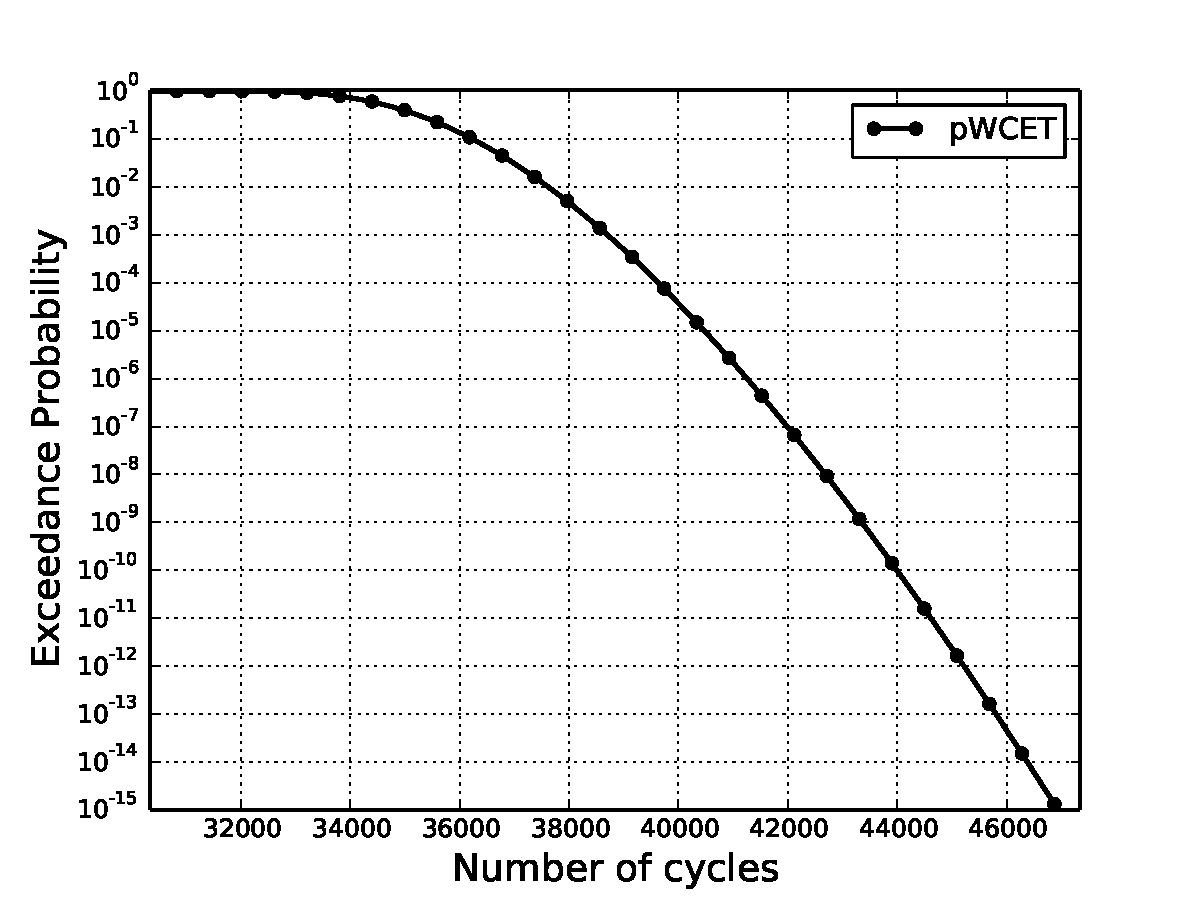
\includegraphics[scale=0.75]{figures/pwcet.pdf}
\caption{Exceedance Probability.}
\label{exceedance}
\end{figure}

 

\subsection{Measurement-Based Probabilistic Timing Analysis}

Measurement-based probabilistic timing analysis is a technique used to reduce the cost of acquiring the knowledge needed to compute trustworthy WCET bounds~\cite{hansen2009statistical, cucu2012measurement, kosmidis2014pub}. MBPTA approach determines the WCET estimates for an arbitrarily low probability of exceedance --- named probabilistic WCET or pWCET. This technique is based on the Extreme Value Theory (EVT) and provides an estimation of the WCET of a task or application running on a hardware platform. In order to defeat the dependence on the execution history, this technique employs randomization in hardware structure. For this, MBPTA technique uses the theory of rare events~\cite{Cazorla:2013:PPA:2465787.2465796}. There are two rare event theories which fits the WCET estimation: \textit{theory of extreme values}~\cite{gumbel1954statistical} and \textit{theory of large deviations}~\cite{gumbel1954statistical}. To the best of our knowledge, EVT is the only theory implemented so far for WCET estimation. The EVT provides an estimation for the maximum of a sequence that consists of independent and identically distributed random variables~\cite{hoeffding1963probability}. The EVT can be used to provide the average execution-time and worst case execution-time of the program or software~\cite{cazorla2013upper,anwar2015probabilistically}. The EVT is mainly used for the statistical purpose~\cite{gumbel1954statistical} along with Block Maxima \cite{gumbel1954statistical} which is used to select highest execution-time and  peak over threshold~\cite{gumbel1954statistical} which is also used to measure highest execution-time. Mainly, the EVT is used on time deterministic architectures for WCET computations. In this work, we used EVT on time randomized hardware for WCET bound.

\subsection{Extreme Value Theory for MBPTA}


Extreme value theory is used to find the probability of rare events. The EVT has been used in the past to find the average and the worst case execution-time of software programs~\cite{altmeyer:spta}. The EVT has used to find the pWCET that upper bounds the execution-time of the program. It also computes cumulative distribution function with the guarantee that the execution-time of the program only exceeds the given bound with a probability lower than a threshold, e.g. $10^{-15}$.  


In order to use EVT for MBPTA, we need to give special treatment to the timing values that would be observed by running the application/software program on a processor. The timing values should be regarded as random variables that must have i.i.d property.  We used EVT to predict the maximum execution-time in a set of observations. There are two ways to perform EVT on timing values. The first approach is Peak over Threshold method~\cite{cazorla2013upper} which models the distribution of timing values over a certain threshold. In this case, limiting the distribution of exceedance probability can be shown by using generalized pareto distribution (GPD). The second approach for EVT considers the largest (maximum) observation among the successive periods. The maximum distribution is modelled to follow one of the Gumbel, Frechet or Weibull distributions~\cite{gumbel1954statistical}. We used Gumbel distribution to model our timing values as shown in Figure~\ref{gumbel}.

\begin{figure}[tb!]
\centering
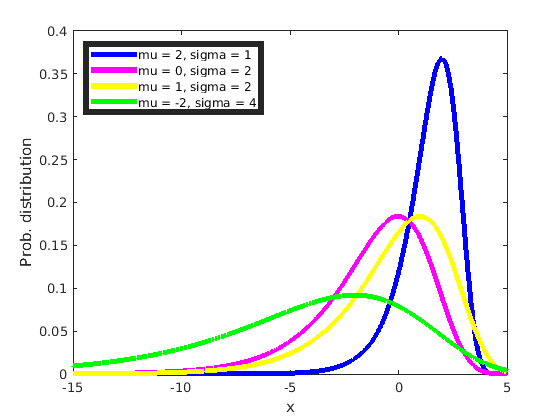
\includegraphics[scale=1]{figures/gumbel.png}
\caption{Gumbel Distribution.}
\label{gumbel}
\end{figure}





\subsubsection{Usage of EVT for WCET estimation}
The EVT is used to predict the worst case execution-time of the applications running on the processor. The inputs of EVT are the numbers of observations which are derived from the real execution of the code. Then EVT gives us the probabilistic prediction of the worst execution-time as shown in Figure\ref{evt-process}.  However, there is a requirement associated with the observed values that the observed timing values should have, i.i.d property. The i.i.d  property is associated with random variables. The independent property states \textit{"Two random variables are said to be independent if they describe two events such that the occurrence of one event does not have any impact on the occurrence of the other"}. In addition, identical property states \textit{two random variables are said to be identically distributed if they have the same probability distribution function}. In our case, the timing values are considered as random variables which the occurrence runs (execution-times) are independent of each other.  EVT does not depend on  how timing values are derived as it considers it as a black box as shown in Figure\ref{evt-process}. Timing values should follow i.i.d property to apply EVT to get pWCET. But the requirement for i.i.d puts some requirements and restrictions on the hardware platform, i.e. the hardware components are randomized which would facilitate the i.i.d property to timing values. We discuss this issue in detail in the next section. 

\begin{figure}[tb!]
\centering
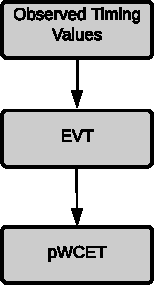
\includegraphics[width=0.25\textwidth]{figures/EVT-Process.pdf}
\caption{EVT-Computing System.}
\label{evt-process}
\end{figure}
 
\subsection{Achieving Time Randomization}
\label{ATR}
%\textbf{MBPTA requirements}

MBPTA considers events resulting from the observation of end-to-end measurements of the program. As discussed above, MBPTA uses a statistical method EVT to compute a probabilistic WCET estimate. Therefore, it requires that the observed execution-times are probabilistically independent events. The requirement for EVT is that: the execution-times of a program run (on the same path) have a distinct probability of occurrence and can be modelled with an independent random variable. This technique is being used for the analysis of cache and processor architectures~\cite{kosmidis2014measurement, mezzetti2015randomized}. We also use this technique for the WCET prediction which we discuss in Chapter \ref{sec:paper1}.  One way to achieve the time randomization is to vary memory layout of the program and data that affects the program execution-time. This is a software-level technique to create randomization.  But this approach is not very common in  practice to achieve randomization since it puts extra burden on the user. The MBPTA technique can facilitate randomization by randomizing the placement and replacement policies which helps to make the overall system probabilistically analyzable. This approach achieves randomization at hardware level by changing the design of the cache. The random placement and replacement policies breaks the dependencies in which the index-set of the data is changed at every run. In this manner, designers do not need to control the location of the data in memory. The observed execution-times can be regarded as i.i.d random variables so that EVT can be applied.

\subsection{Static Probabilistic Timing Analysis Technique}
\label{static}

The static version of PTA is SPTA that uses a model of a processor to derive a priori probabilities for the latency of the program instructions running on a processor~\cite{bernat2002wcet}. This technique has been the recent subject of many studies~\cite{Cazorla:2013:PPA:2465787.2465796, davis2013analysis, altmeyer2014correctness, bernat2002wcet}. In SPTA, the execution-time of a probability distribution for an individual instruction is determined statically from a processor model~\cite{Kosmidis:2013:CDP:2485288.2485416}. It means that the probabilities for the execution-time of each instruction are independent. Whether an executed instruction is a cache hit, or a cache miss, it does not affect the probabilities of later instructions on a queue. Each instruction derives its own probabilistic timing behavior represented with the help of an execution-time profile (ETP). The ETP of an instruction is expressed as $ETP(I_i)=<\vec{t}_i, \vec{p}_i>$
where $\vec{t}_i=(t^1_i, t^2_i,...,t^n_i )$ and $\vec{p}_i=(p^1_i, p^2_i,...,p^N_i)$, with  $\sum^{N{_i}}_{j=1}{p_i}^{N_j} = 1$. The convolution function is used to combine all the ETPs of the instructions to obtain the new ETP, which is used to represent the time distribution of all convolved instructions. The probabilistic cache with evict-on-miss random replacement policy is introduced
to reduced WCET of the system and it works in this way: when a cache miss
happens, a cache block is selected randomly for the new entry from the main
memory. Different from Least Recently Used (LRU) replacement policy, this random
behavior avoids cases with low pathological occurrence probabilities which are
hard to test and predict such as~\cite{Cazorla:2013:PPA:2465787.2465796}. Therefore the
WCET can be improved.
Several formulae have been proposed for SPTA analysis of probabilistic caches.
\cite{zhou:spta} uses \textit{reuse window} to calculate a probability of each
memory address access but this has been proved unsound by \cite{Cazorla:2013:PPA:2465787.2465796}. This is because, during the probability calculation, memory
accesses are not independent of one another. Due to lack of this independence,
the result of his formula cannot be used in some cases. \cite{Cazorla:2013:PPA:2465787.2465796} proposed another formula for SPTA, as shown
in equation~\eqref{eq1:test}. In this formula, \textit{N} is cache associativity and \textit{K} are
\textit{reused distance}. \textit{Reuse distance} represents the number of memory
addresses between two continuous accesses to the same memory address.


\begin{equation}\label{eq1:test}
P(hit) = \left\{
\begin{array}{l l}
(\frac{N-(K-1)-1}{N-(K-1)})^K & \quad if K<N\\
0 & \quad if K\geq N\\
\end{array}
\right.
\end{equation}

%Consider an example let have two random variables denoted by $\textit{X}$ and $\textit{Y}$ used to describe the execution-time profile of two instructions denoted by \textit{x} and \textit{y}. We can use the convolution function to  find the ETP $\textit{Z} = \textit{X} \otimes \textit{Y}$. 

Equation~\eqref{eq1:test} represents the hit probability of each memory address in
the cache. This equation takes the number of cache entries into account and when
\textit{reuse distance} is beyond its scope, the hit probability is 0. By using
equation~\eqref{eq1:test}, the pessimistic probabilities of all memory addresses are
obtained and are independent of each other. Therefore, the overall
probability distribution can be calculated by convolution of all probabilities. Execution Time Profile (ETP), as shown is equation \eqref{eq2}, is used to represent timing information (numbers of cycles) and its
associated probability. 


%In this work, the number of cycles is applied as
%timing information and thus we have  
\begin{equation}\label{eq2}
ETP = \{(c_1, c_2, ...), (p_1, p_2, ...)\} 
\end{equation}

Where $c_i$ is the numbers of cycles, and $p_i$ is its corresponding occurrence
probability.
\\
Consider an example; suppose there are two ETPs: 
\begin{center}


$ETP_1 = \{(1, 2, 3), (0.1, 0.3, 0.6)\}$ \\
$ETP_2 = \{(1, 3), (0.2, 0.8)\}$
\end{center}

From SPTA, we can compute their convolution: 
\begin{center}
$ETP_1 \otimes  ETP_2 = \{(1, 2, 3), (0.1, 0.3, 0.6)\} \otimes \{(1, 3), (0.2, 0.8)\}$ \\
$ETP = \{(2, 3, 4, 5, 6), (0.02, 0.06, 0.2, 0.24, 0.48)\}$
\end{center}

\textbf{Drawbacks}
\begin{itemize}
\item To determine the execution history, SPTA requires a detailed knowledge of hardware and software. This knowledge is hard to model due to intellectual property restrictions or hindered documentation. Any reduction in available knowledge leads to a rapid degradation of the tightness of the WCET estimation. 
\item MBPTA works for complex processor architecture. Whereas, SPTA works only for simple processor architectures~\cite{abella2014comparison}.
\end{itemize}


The relevance of a PTA to our research is represented by the proposition of a taxonomy and a general framework for accurate WCET prediction for the aerospace computing systems. The primary motivation of this technique is to cope with the history dependency which is highly desired due to the steadily growing complexity of modern computers.


\subsection{Comparison Between Measurement and Static Probabilistic Timing Techniques}
\label{properties}

Probabilistic timing analysis pursues the goal of achieving \small{p}WCET estimation through static and measurement-based techniques: 
\begin{itemize}
\item {The execution-time of the application can be accurately modelled at some level of execution granularity by a probability distribution}. 
\item {Probabilistic timing analysis attacks the timing wall}.
\item {Probabilistic timing analysis reduces the extent of knowledge about the execution platform required to produce probabilistically accurate WCET estimations}.
\item {Probabilistic timing analysis aims to obtain pWCET estimates for an arbitrarily low probability so that even if pWCET estimates are exceeded, it would be exceeded with low probabilities}.
\end{itemize}





Starting with the efforts on timing analysis using the probabilistic cache, several different cache models are proposed.~\cite{quinones2009using} proposed a randomized replacement policy for standard and skewed associative caches which improves WCET at the cost of degrading performance for the best cases. For a different approach,~\cite{kosmidis2014measurement} proposed a software method for
conventional caches. It modifies memory objects offline using  compilers and linkers or
online using program loader and runtime libraries.
There are two techniques for probabilistic cache timing analysis. The first technique is SPTA. Reuse distance, cache associativity, and entry cache numbers are usually used for calculation.~\cite{zhou:spta} proposed a cache hit formula using reuse distance which simplifies computational complexity. The probabilities for each cache
access are made independent and the final result is the convolution of all cache accesses.


However, his methodology has been found faulty~\cite{Cazorla:2013:PPA:2465787.2465796, altmeyer:spta} Another formula is given by~\cite{Kosmidis:2013:CDP:2485288.2485416}, which may overestimate the cache hit ratio ~\cite{davis:improve}. Thus, the result of probabilities for timing may be too optimistic and incorrect. ~\cite{davis2013analysis} developed a formula to estimate WCET, assuming the reuse distance is known, which is proved to be optimal by~\cite{altmeyer:spta} with limited information. Besides, an exhaustive analysis approach as opposed to a simplified formula is proposed in~\cite{altmeyer:spta}. To reduce the computational complexity, the comprehensive approach can be combined with simplified equations. As computational complexity increases, the result is more accurate, but its
calculation time grows as well.
Apart from SPTA, the MBPTA methodology based on EVT assuming independent and identically distributed random property is tested and Gumbel distribution function is proved to fit the distribution. With these assumptions, result from EVT
shows that this technique is close to SPTA. Besides, with mathematical
techniques, only a few hundred simulations are required for calculation.

\subsection{TIME-PREDICTABLE ARCHITECTURES}

This chapter discusses a design methodology for time-predictable architectures. In this chapter, we discuss how time-predictable designs are different from general purpose processor architectures. We also discuss different probabilistic systems such as a probabilistically analyzable cache and bus. We propose the method of achieving the objectives of our research, i.e. the implementation of probabilistically analyzable, time-predictable computing systems.

%%
%In addition to the development of our research along these axes, we also have a plan to implement a technology demostrator on FPGA and, possibly, a CubeSat platform.

\subsection{Time-Predictable Architecture}


As we know, computing systems that are subject to respond to strict operational deadlines from events, (i.e. alarms, commands,
etc.)  are called real-time systems. These are employed in many applications where the response time of a control system can have a critical impact on the safety of people or infrastructure, (e.g. airplanes, automobiles, and satellites). As critical applications become more and more complex, the performance of real-time systems has to increase to guarantee appropriate safety standards. The main obstacle to high-performance real-time systems is the unpredictable timing behaviour of the modern computer architectures. Currently, software designed for real-time systems needs to be guaranteed to be executed within the required time frame. Depending on the complexity of the underlying hardware architecture, this level of certainty might be difficult or impossible to reach. Within this context, this project will introduce a probabilistic approach: by enabling true randomized behaviour in processors and memory architectures, one can define
probabilistic metrics for the timing behaviour of a system. This would bring real-time software engineering in line with other engineering domains that perform risk analysis using component failure probabilities. 

However, there are few time-predictable architecture available based on the deterministic timing analysis, e.g. the multithreaded processor \textit{Komodo}~\cite{kreuzinger1999komodo}. The \textit{Komodo} processor core is used to execute Java applications natively. This processor assesses the memory at higher clock frequency than for the pipeline. This technique facilitates the pipeline to access the memory in a single pipeline cycle leading to a precisely predictable access time. There is one more processor for Java applications named Java optimized processor~\cite{Schoeberl:2009:TCA:1540555.1554265}. This processor takes advantages regarding predictability over the conventional processors. This processor introduced stack cache and method cache that prevents additional runtime stack, save/store procedures of the register file, prevents memory conflicts. These two above mentioned processors are based on single core architecture.  There is a multicore processor architecture named \textit{MERASA}~\cite{ungerer2010merasa} used to parallel execution of multithreaded with hard real-time requirements. Static and measurement-based WCET analysis techniques are supported by  \textit{MERASA}. The \textit{MERASA} is based on a central cache configuration that can be used to assign with required number of cores used to execute a multithreaded application. These processors used deterministic timing techniques for WCET estimation, and their architectures are also deterministic.

Realization of a time-predictable computer architecture --- it's definition, modification of a current processor architecture, and implementation is a domain of real-time systems research. Real-time processor architecture needs a reasonable and known WCET that makes it different from the general purpose processors. Classical enhancement are harder to model a system which gives an accurate prediction for WCET measurement. The key factors for performance enhancements such that knowledge of an execution history,  mainly an issue for the WCET analysis. Therefore, we need to develop new techniques to design a processor for WCET estimation. We do not want to restrict the features but also want to actively add features that enhance performance and time predictability. PTA techniques are newly invented methods which are less dependent on having an execution history. In this work, our main focus will be on circulating around the improvement and inventing of new architectural features, i.e a randomized cache for better WCET estimations.

\begin{figure}[tb!]

 \centering
%  \captionsetup{justification=centering}    
   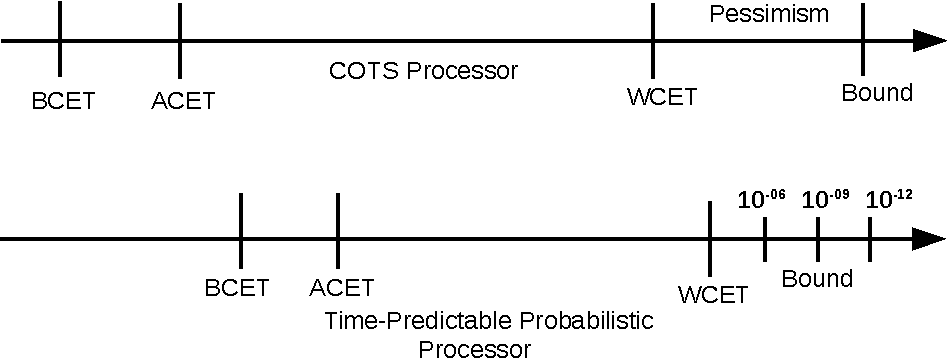
\includegraphics[scale=1.0]{figures/tpc-thesis.pdf}
   \caption{Timing Distribution of different Architectures.}
\label{fig:tpc1}
\end{figure}





Figure~\ref{fig:tpc1} shows the purpose of a time-predictable architecture. Figure~\ref{fig:tpc1} shows the best case execution-time (BCET), average case execution-time (ACET), and WCET bounds for tasks executing on different architectures~\cite{schoeberl2009time}. The difference between the actual WCET and the bound is caused by the pessimism of the timing analysis already discussed in section~\ref{sec:intro}. In figure~\ref{fig:tpc1} the first time line shows the execution-times for a commercial off-the-shelf (COTS) processor. The other two time lines show the timing for two different time-predictable processors.
The Time-predictable processor has a higher BCET, ACET, and WCET than a
COTS processor. However, the WCET is higher than the WCET of the COTS processor, the
pessimism of the analysis is lower and the resulting WCET bound is lower as well. Even this type of
processor is a better fit for critical real-time systems than today’s standard processors.
The Time-predictable processor shows an architecture where the BCET and ACET are worst than the COTS processor, but the
WCET and the WCET bound are decreased with the probability of exceedance that is defined as: the probability of exceeding a given pWCET. Our goal is to design an architecture with a low WCET
bound whose predictability is closer to the real execution-time. For critical real-time systems, the likely increase in the ACET and BCET is acceptable, because
the complete system needs to be designed to reduce the WCET bound and improve predictability. It should be noted that a processor
designed for low WCET will never be as fast as a processor designed for performance improvement of ACET~\cite{schoeberl2009time}. In this research project, the randomized cache component is designed to facilitate the  standard processor for WCET analysis. However, there are some other architectural modifications, e.g. randomized branch prediction also helps prediction. We did not implement them but provide this as a suggestion to help future researcher to take this project to the next level.

\begin{figure}[tb!]

 %\centering
  %\captionsetup{justification=centering}    
   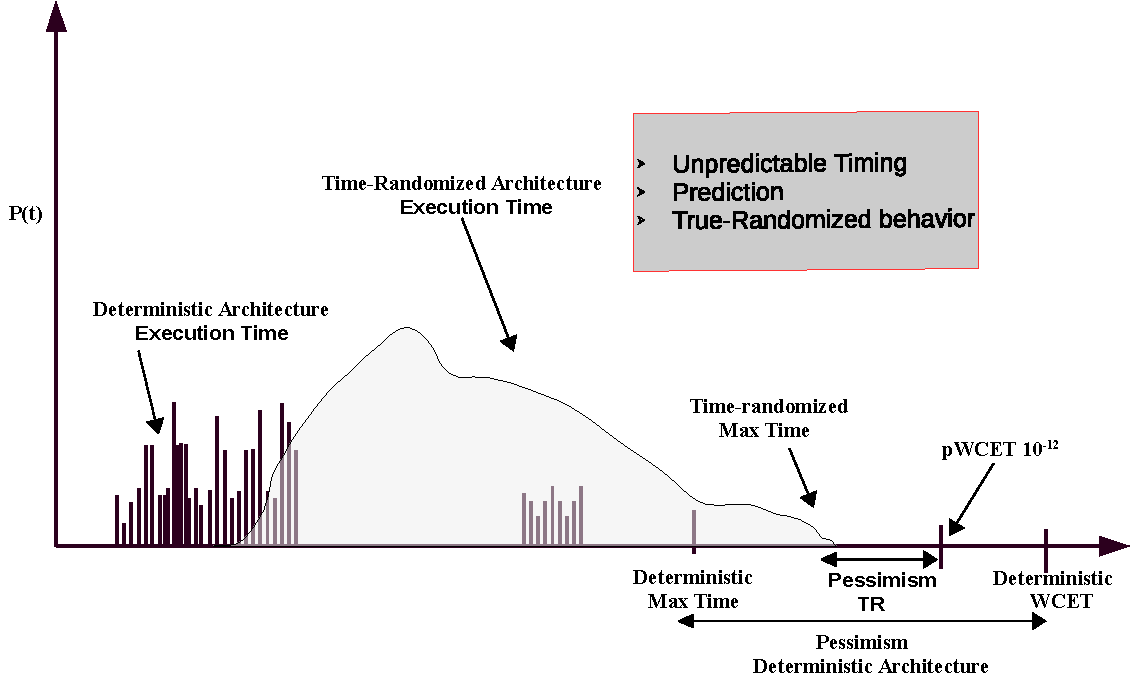
\includegraphics[scale=0.77]{figures/pta-new-crop.pdf}
   \caption{Probability Density Probabilistic Architectures: avoiding corner cases will
improve WCET Estimation and Bound the Execution-Time t with Probability P ($t$ > $t_x$ ).}
\label{fig:prb}
\end{figure}

\begin{figure}[tb!]

% \centering
 % \captionsetup{justification=centering}    
   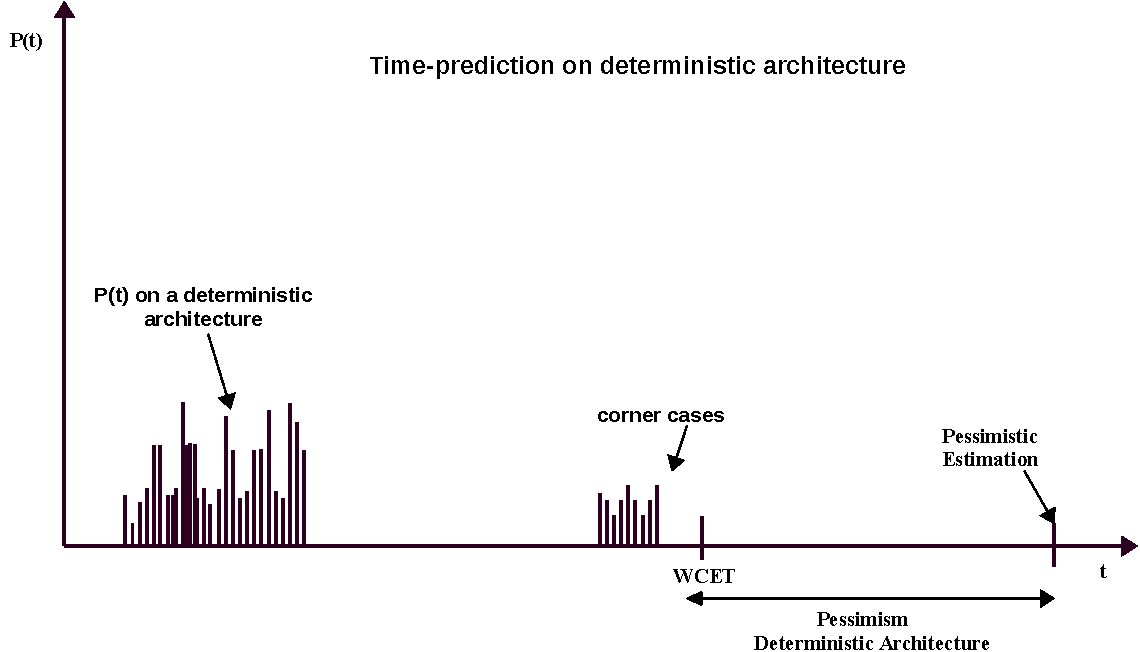
\includegraphics[scale=0.77]{figures/pta-det.pdf}
   \caption{Probability Density for Deterministic Architectures.}
\label{fig:det}
\end{figure}






Figure~\ref{fig:prb} shows how the idea of the probabilistic system that might affects the verification of real-time systems. Consider a satellite on-board computer: the Y-axis shows the probability density (P (t)) of a given execution-time t on
the X-axis for a particular task (e.g. sending telemetry data) running on the on-board computer. Normally
the execution-time of an application on a deterministic architecture follows a distribution that might have
some corner cases as shown in Figure~\ref{fig:det}. A conservative estimation will place the WCET far away from the actual maximum
time used by the application, especially when considering possible interactions with other tasks. This would
lead to a large overestimation of the computing resources needed for the task. Instead, a fully probabilistic
architecture will have a lower performance on average since current computer architectures are optimized
for the average case, but a much smoother distribution, with a single bell curve. Using our methodology, the
maximum execution-time t can be smoothly estimated as a probability function, e.g. P (t > t max ) = $10^{-12}$.
The overestimation of the needed computing resources will be greatly reduced, as well as the cost of determining the WCET for every task. In addition, the combined effect of multiple tasks (e.g. housekeeping,
attitude control, etc.) will be predictable without re-analyzing the complete system. In practice, this can
reduce cost for the timing analysis of a critical system by several orders of magnitude.
Bringing real-time systems development at the same level as any other domain of engineering will have
a tremendous impact on the cost of production, verification and certification. As a whole, this research
program will enhance the competitiveness of the Canadian aerospace industry: companies like MDA and
Bombardier Aerospace could take advantage of the new probabilistic real-time systems for the development
and reduced certification cost of spacecraft, high-altitude planes, and unmanned air vehicles.

\subsection{Architectural Modifications}
\label{AM}
In order to develop a time-predictable computer architecture, we will need to modify the following architectural components/features of a current processor architecture.
For the purpose of this work, few key arguments for a time-predictable computer architecture development are presented below. 

\begin{itemize}

\item  Pipelines will be simple, with minimum dependencies between instructions.

%\item  As we known, caches are mandatory  to bridge the gap between a processor speed and a memory access time. Cache usage makes WCET analyses complex. Therefore, we need different cache designs, like;  using \textit{randomized cache} which helps to drive tighter WCET analysis

\item  Avoid processor's out-of-order execution and speculation as it increases WCET complexity.

\item  In-order to avoid an unbounded timing effect, time-predictable processors use prefetch queue and double buffer.

\item Use static branch prediction instead of dynamic predictors.

\item  To avoid inter-thread interference, need to develop a policy by using one thread per processor. This philosophy will remove the classic schedulability analysis and we need to do scheduling of a memory access.

\item Inter-core interference via shared memory is also a problem for WCET analysis. To avoid this, develop a policy, e.g. randomized Time Division Multiplexing Access (TDMA) scheduled memory access.

\end{itemize}


\subsection{Probabilistically Analyzable Single-core Architecture}

Time-predictable computing systems fulfills the requirement of a real-time computing systems. We will need to perform a probabilistic analysis on each of the architectural components (processor, memory, and NoC) for accurate prediction of WCET. In this project we implemented  the definition of a novel probabilistic architectures on an FPGA that will prove the applicability of the approach to space applications. One of the main obstacles to high-performance real-time  systems is the unpredictable timing behaviour of the modern
computer architectures; with multi-stage pipelines and three-level memory hierarchies, it is extremely difficult to accurately predict the execution-time of a given program. This is almost impossible with parallel (such as multi-core) architectures, due to the presence of the shared resources. Being conservative and over-estimating does not solve the problem because of the extremely large difference between the  worst
and the average cases. The design of powerful real-time systems needs a new approach for the architecture
of instruction processors. In this context, we propose a probabilistic analysis approach: by enabling true randomized behaviour in all the components of a computer, one can define probabilistic metrics to the timing behaviour of a system. Successful implementation of such systems will have tremendous impact on the way critical systems are designed, and the potential benefits are enormous in terms of cost of integration, verification, and certification of real-time software. Probabilistic
analysis of a computer architecture is introduced by the PROARTIS European Project~\cite{Cazorla:2013:PPA:2465787.2465796}. PROARTIS focuses on worst case execution-time
(WCET) and proposes targeted modifications to hardware modules to improve timing analysis.

%The execution-time of an application or a software running on a deterministic architecture
%follows a distribution that might have some corner cases. A conservative estimation will place the WCET
%far away from the actual measured maximum time used by the application, especially when considering possible
%interactions with other tasks. Due to application interaction, a large over estimation of the computing resources needed for the task. On the other side, a fully probabilistic architecture in general will have a lower performance on average as compared with current computer architecture. As these architectures are optimized and designed for the average case. Moreover, probabilistic architecture have more smoother distribution and looks like 
%a single bell curve.
%
%Using our methodology, the maximum execution-time \textit{t} can be smoothly estimated as
%a probability function, e.g. $P (t > t_{max} )$ = $10^{-12}$ . The WCET for every task and over estimation of the computing resources will be greatly reduced. Moreover, the
%combined effect of a multiple tasks (e.g. housekeeping, attitude control, etc.) will be predictable without
%re-analyzing the complete system. In practice, the timing analysis of a critical
%system is reduced by several orders of magnitude. For timing behavior calculations of a probabilistic system, we have to remove determinism from a 
%computer architecture, because determinism introduces dependencies between instructions that break any
%assumption of a normal distribution of an events. Our approach is to used a true random number generator~\cite{OpenCores} to guarantee the randomness and normal
%distribution of an events for all hardware components.
This research project  focused on the definition and implementation of a randomized computing system, e.g. randomized caches. We implemented the randomized cache and integrated it with MIPS-32 and Leon-3 processor as there  source code are freely available~\cite{leon3, ION} and then implemented as a prototype on FPGA. A true random
number generator will be implemented as well, based on an existing literature~\cite{OpenCores}. This generator will be
used to guarantee a sufficient entropy pool for the complete randomization of the hardware architecture. The final result of this research will be a fully-functional prototype of a time-predictable probabilistic LEON3 on FPGA. We  considered the timing estimation of a program running on the proposed architecture. 
%
%We will explore both timing analysis techniques, SPTA and MBPTA for predicted WCET estimation. Our newly developed processor architecture will be implemented on a Xilinx Virtex-5 / ZyNQ board. We will try to make it fault tolerant to avoid
%the space radiation effects that have potential to disturb the timing behavior, the final architecture
%will be built to provide a certain degree of fault-tolerance. This demonstrator will be implemented in a CubeSat mission and will include a payload fulfilling a scientific mission.

%\section{Research Axis 3: Fault tolerance}

%At high altitude or in space, without the protection of the Earth's magnetic field and
%atmosphere, electronic components are subject to high levels of ionizing and particle radiation
%that can disrupt the correct circuits behavior. The components lifetime is reduced by the
%former, especially at high levels of utilization, and transient errors might be caused by the
%latter. In order to make the system fault tolerant. We need to develop a fault detection and recovery mechanism.

%Mission-critical digital systems are often implemented on FPGAs, which allow for easy reprogramming of the hardware. FPGAs are especially desirable in
%these applications due to their cost-effectiveness for relatively small quantity productions and the ease
%in which they can be updated. The re-programmable nature of FPGAs presents one of its strongest
%advantages as well as one of its most significant limitation as compared to an Application Specific
%Integrated Circuit (ASIC), which is a non-reprogrammable integrated circuit that is customized for a
%particular use. However, this non-permanent characteristic of FPGAs also causes problems with errors
%in the system, especially in environment subject to high radiation. Particles may cause portions of the
%re-programmable circuitry to change states. Therefore, FPGAs are  more prone to errors in its logic
%values and in its actual circuitry than a more permanent custom hardware solution such as an ASIC. In order to make the system fault tolerant. We need to develop a fault detection and recovery mechanism.


%Transient errors can be detected and corrected using memory scrubbing. Detection
%of transient errors and protection against single event upsets (SEUs), or soft errors, can be
%obtained in several ways [47], but there is no predominant or established methodology on
%how to identify permanent faults. One way to do it is to retry the same computation multiple
%times, and, after a certain number of repeated errors in a given interval of time, declare the
%component as permanently faulty

%\subsection{Fault Injection}
%
%We need to study the behaviour of a timing analysis under faults. For fault injection we will follow two strategies: (a) \textit{Software based fault injection}, and (b) \textit{FPGA based fault injection}. 
%
%\begin{itemize}
%
%\item Two methods will develop for software based fault injection. First, the source HDL code is modified in order to allow fault injection. Second, the simulation tool is used to force the error injection during simulation. 
%\item For FPGA based simulation, we will use single error mitigation core from Xilinx~\cite{xilinxsem}. The idea is to integrate this core with our system to generate a modified bitstreams to emulate the occurrence of errors
%\end{itemize}
%
%A probabilistic timing analysis will be done with both SPTA and MBPTA. It helps us to find estimated WCET in the presence of faults.
%
%\subsection{Fault Mitigation}
%Fault-mitigation can be achieved in two ways: preventing faults from happening and
%recovering after their occurrence. Fault preventing is achieved by using hardened components and/or shielding. But fault preventative is not a viable solution in terms of a project cost. More complex fault-mitigation methodologies can be implemented at the architectural level. We need to develop some fault-mitigation strategies like: triple module redundancy with  dynamic reconfiguration of the hardware~\cite{jacobs2012reconfigurable} and/or something like the work presented in 
%%Jacobs \emph{et al.}~\cite{jacobs2012reconfigurable} and Alderighi \emph{et al.}~\cite{violante} promote the use of SRAM-FPGAs for reconfigurable fault-tolerant space applications.
%~\cite{jacobs2012reconfigurable} used fault tolerance framework (RFT) that enables system designers to dynamically adjust a system's level of redundancy and fault mitigation based on the varying radiation incurred at different orbital positions. Notably, the reconfigurable fault tolerance framework in~\cite{jacobs2012reconfigurable} is based on an upset rate modeling tool that used to capture time-varying radiation effects in a given orbit.
\subsection{Probabilistic Multi-core Architecture}

This work is focused on the single-core architecture. 
Designing multi-core processor for WCET bound is an interesting idea. Here, we present a general approach and challenges associated to design a probabilistic multi-core architecture. Determination of WCET of applications executing on shared memory multi-core processors is hard to estimate. This hinders the adoption of multi-core processors in CRTES~\cite{Jalle:2014:BDT:2616606.2616668}. We need to develop new timing analysis technique which empowers WCET measurements on multi-core architectures. Most existing multi-core processors contain one shared, usually last-level cache (LLC). This holds for processors used in critical and real-time systems, like the ARM Cortex A9 and A15, the Freescale P4080, and the Aeroex Gaisler NGMP. While, an LLC offers a
high potential for average performance improvement, it increases the complexity of a 
worst-case execution-time  estimation, which has made LLC to be studied in the
last years by the real-time community. This is due to the difficulty of determining which
memory accesses will hit the cache and which will cause cache misses. This information is necessary to
drive tight WCET estimates. Classifying cache accesses as a hit or a miss in non-shared
caches has been already deemed as a complex process, subject to some degree of
pessimism, therefore reducing the tightness of the estimated WCET bounds. This is
even more complex with LLC, in which the main challenge for WCET estimation is an inter-task interference. The solution based on
extending the WCET estimation process to the coordinated analysis of several tasks
simultaneously sharing a LLC is a complex task. Alternatively, preventing inter-task
interference by deploying cache partitioning techniques is the preferred solutions in real
time systems to deploy LLC. This solution, however, introduces fragmentation in the
use of the memory and may require significant changes in the memory management.
Moreover, partitioning increases the complexity of the data sharing across tasks and task
scheduling. These challenges highlight a need to explore a new type of cache, and how it can be
used as LLC, in particular, need to consider time-randomised  caches, which allow
controlling inter-task interference without cache partitioning. This is the principle behind TR-LLC.
A TR-LLC cache removes any dependency on the particular addresses accessed and
its assigned cache set. Therefore, the LLC interference  only depends
on how often (frequency) its co-runner tasks cause a cache miss, and not the particular
address generating the miss. As a result, controlling eviction frequency in a TR-LLC by
delaying the time at which misses are served for each task  is enough to dependably
upper-bound the maximum effect in the LLC that a task may have on all other co-runners. Hence existing multi-core processor with an LLC can be use and
need to design a hardware mechanism that limits the miss frequency of tasks in each core at
analysis and deployment time. This will be done in such a way that the probabilistic upper-bounds can be obtained for inter-task effects in the LLC. 

\subsection{Probabilistically Analyzable Real-time Systems}


Aiming at the development of a full probabilistic analyzable time-predictable computing system is a main focus for a research community. 
We cannot neglect the fact that such computing systems have stringent real-time requirements. Enforcing real-time requirements in a  multi-processor system-on-chip (MPSoC) is a particularly challenging task. The probabilistically real-time systems are those system, where meeting the deadline is the first order priority~\cite{schoeberl2011towards}. Chances for missing the deadline is probabilistically arguable with target probabilities of $10^{-6}$, $10^{-12}$, etc. Real-time systems are becoming vital in applications such as flight control system, and modern cars where wires harnesses are replaced by bus, switches are replaced by smart switches engine and other functionalities of the car are controlled by the processors. Since, these system are designed to work in an extreme conditions, meeting the deadline for a particular operation, (e.g. opening of an air bag in the case of an accident should follow strict time deadlines that is very important for such life saving applications). The timing analysis poses the fundamental importance in real-time systems to accurately measure the WCET of a software/program running on it. The usage of a probabilistically analyzable real time system and especially worst case execution-time analysis allows to strongly reduce the over estimation produced by traditional timing analysis method. So far, the researchers have been focused on a probabilistically analyzable processor, cache, bus, and memory. But the whole system didn't probabilistically analysed. In the following sub-sections, a general overview of all each sub-system is presented. 




%Traditional approaches for worst case execution-time (WCET) analysis aim at finding the absolute upper bound on the execution-time. For modern high performance processors with, for example, out-of-order execution, these technique may produce estimates for the WCET which are pessimistic due to the simplifications that may need to be made and due to the inherent variability of the execution-time. In addition, end to end measurements as used in industry produce estimates of the execution-time that potentially underestimate the real worst case execution-time.
%
%We introduce the notion of probabilistic hard real-time system as a system which has to meet all the deadlines but for which a (high) probabilistic guarantee suffices.
%
%pWCET combines both measurement and analytical approaches into a model for computing probabilistically bounds on the execution-time of the worst case path of sections of code. 
\subsection{Probabilistically Analyzable Cache}

Previous works deal with the probabilistically analyzable cache, processor, and communication infrastructure~\cite{mezzetti2015randomized, cucu2012measurement, Jalle:2014:BDT:2616606.2616668}. In these papers, authors used the concept of time randomization to achieve the requirements for a probabilistically analyzable real-time systems. Because deterministic nature of placement and replacement policies makes it impossible to drive true probabilities for different execution-times. However, the usage of probabilistic cache increased complexity, energy, and performance of the system. But the benefit achieved regarding prediction by employing probabilistic cache is unparalleled. Authors enabled the usage of set-associative and direct mapped cache in the context of probabilistic timing analysis. They proved in their work how their design and methodology drastically reduce the information required by the analysis to drive WCET estimations. Authors encountered both approaches for measuring the WCET analysis: end-to-end
measurements of instruction counts, or static techniques based on
a source code analysis~\cite{Wilhelm:2008:WEP:1347375.1347389}.  Both
techniques are limited: static techniques work only on a simple hardware
architectures and end-to-end measurements technique quickly loses its accuracy
as software becomes more complex.  In particular, the behaviour of a cache memory is a serious obstacle for the  implementation of these
techniques. Deterministic caches are hard to predict because they are geared
towards improving the average
cases~\cite{Kosmidis:2013:CDP:2485288.2485416, Topham:1999:RCP:297703.297715} used a random placement based on
a parametric hash function to avoid conflict misses to improve
the average cases. And, without considerin the real-time systems.~\cite{Reineke:2007:TPC:1290860.1290864} shows the impact of different
cache policies on a WCET estimation, but without considering random
replacement policies.~\cite{ARM} used randomized cache to make processing system more predictable. 
~\cite{David:2004:SDP:1009383.1009841} introduces Static Probabilistic
Timing Analysis (SPTA) for WCET estimation, but without any hardware support.~\cite{cucu2012measurement} presents Measurement-Based Probabilistic
Timing Analysis (MBTPA) assuming the existence of probabilistic hardware
but without any actual implementation.~\cite{Cazorla:2013:PPA:2465787.2465796} introduces the concept of
probabilistically analyzable caches, but does not provide a cache
implementation. These caches are based on random placement and
replacement. Kosmidis presents a simulation of a probabilistic cache, and shows
that it can be used for SPTA and
MBPTA~\cite{Kosmidis:2013:CDP:2485288.2485416}.   

In~\cite{quinones2009using}, the usage of randomized cache over the deterministic one is demonstrated. They first used the standard cache replacement policy and observed a point comes in a simulation where cache miss rate is high enough that it effectively disable the cache usage. On the other side randomized cache successfully removed the pathological behaviors and achieved reasonable performance. This paper is first of its kind to use randomized cache which helps predictability for real-time systems. 

~\cite{kosmidis2014measurement} this paper extend the concept of applying MBPTA technique to the processor by applying it on cache and  bus. In this paper, authors showed how to drive the probabilities and drive ETP for every program instruction. 


 Although there is argument provided in ~\cite{reineke2014randomized} that randomized cache are harmful in hard real-time systems, author claimed that traditional cache analysis method outperforms the SPTA analysis applied on cache with random replacement, but this argument is answered by the~\cite{mezzetti2015randomized} that applicability of PTA depends on the particular hardware and software conditions, i.e. randomized cache with MBPTA technique  provides tight and trustworthy WCET estimates and DTA performs better on deterministic architecture. In short, deterministic analysis on the top of conventional cache or probabilistic analysis on the top of randomized cache is highly dependent on the particular characteristics of the hardware.  



\subsection{Probabilistic Analyzable Bus} 


Most of the work done so far for a probabilistic analyzable bus for multi-core systems are focused on the bus arbitration policies~\cite{lahiri2001lotterybus, udipi2010towards}. But these bus policies are based on the fixed latency or bounded transactions which are not the case for real-time systems. Advance hierarchy bus (AHB) bus~\cite{ARM} based system focused on the efficient implementations of the RTL models. For example,~\cite{conti2004performance} discussed several arbitration policies regarding latency and power dissipation. In recent years, we have seen very less amount of research focused on a probabilistically analyzable bus. The work accomplished in~\cite{Jalle:2014:BDT:2616606.2616668} is based on a probabilistically analyzable bus design for the multi-core processors. In~\cite{jalle2014ahrb}, authors have achieved the analytical models of the probabilistic timing behavior for different bus designs. They showed PTA suitability. They proved that the bus design for a probabilistically analyzable system fulfilled all the requirements for the probabilistic systems. The bus drives WCET estimates with the same cost and complexity as in single-core processor. The achieved performance enhancement is 3.4 times for 8-cores and 6.6 times for 16-cores in comparison to single core performance. This paper, that was published in $2014$ means a lot of potential left in this research topic, i.e. comparison of many different bus arbitration policies, (e.g. lotter, random-permutations, and multi-bandwidth bus arbitration). Javier Jalle \emph{et al.}~\cite{Jalle:2014:BDT:2616606.2616668} analysed and extended the Advanced Microcontroller Bus Architecture (AMBA)~\cite{jalle2014ahrb} to enable time-composable WCET estimates by design. In this work, they modified the AMBA Advanced High-performance Bus (AHB) named \textit{Advanced High performance Real-time Bus} which allows getting time  composable and tight WCET estimates. 

 

\subsection{Time-Predictable Real-time systems}


Despite the fact that the COTS processors are better than customized processors, the real-time systems community prefers to use a processor with a lower WCET bound~\cite{bate2001use}. Few research projects exist in the field of optimizing the hardware for WCET analysis~\cite {thiele2004design}. A  new research discipline is needed for time-predictable real-time systems which facilitate the concepts with techniques to improve analyzability to drive safe bounds on WCETs.
All architectural components (processor, caches, memory, and bus) of a system need to be time-predictable.
Critical real-time systems need to be time-predictable to prove the timeliness of all their time critical response~\cite{kirner2010time}. There is no general definition for the term \textit{time predictability}. However, there are few time-predictable processors that exist in the literature. Among them, the most recent is a java optimized processor proposed by Martin Schoeberl~\cite{schoeberl2009time}. They have identified the problematic micro-architectural features of the standard processors and provide some alternative solutions. But their architectural enhancements are not yet implemented and tested on RISC based architectues. The use of java optimized processors for space applications is not feasible because of less data available in the market for verification and testing.

Similarly, Edwards \emph{et al.}~\cite{edwards2007case} argue that :\textit{"It is a time for the new era of processors whose temporal behavior is as easily controlled as their logical function"}. Berg et al.~\cite {berg2004requirements} define the time-predictable processor as: \textit{"recoverability from information loss in the analysis, minimal variations of the instruction timing, non interference between processor components, deterministic processor behavior, and comprehensive documentation"}. The author has proposed a five stage pipeline RISC processor, but this processor was not discussed in the context of WCET framework. 

~\cite{heckmann2003influence} provides the basic design strategy for a time-predictable processor: (1) separate data and instruction caches; (2) local update strategy for caches; (3) static branch prediction; and (4) limited out of order execution. But the author did not provide suggestions for additional or alternative features for a time-predictable processor. Although there are more few processors in this domain like VISA~\cite{anantaraman2003virtual}, SPEAR ~\cite{delvai2003processor}, and ~\cite{whitham2008real} these processors have different architectural features to support time predictability but none of them is analysed probabilistically.

Finally, a recent published paper~\cite {schoeberl:timememory} paper presents a solution for the time-predictable
memory arbitration for a chip-multiprocessors. The memory of network-on-chip (NoC)
is organized as a tree with time-division multiplexing (TDM) of accesses to the shared
memory. The TDM based arbitration completely decouples processor cores and allows WCET
analysis of the memory accesses on the individual cores without considering the tasks on the other
cores. Furthermore, performed local, distributed arbitration according to the global TDM
schedule. This solution avoids a central arbiter and scales to a large number of processors. A time-division multiplexing (TDM) arbiter is time-predictable.
It allows for calculation of the WCET of a task executing on one processor core independently from tasks executing on other cores. However, this paper did not discuss the feasibility of calculating WCET on their design platform.

The work presented in \cite{abella2014comparison} is based on the qualitative comparison of different timing techniques with different software and hardware configurations, and provides data to the user to choose particular hardware configuration with suitable timing techniques according to the desired level of pessimism. However, the safeness of WCET bound is not guaranteed due to the presence of discontinuous pathological cache patterns and variation of input test cases may affect the safe bound. 



Similarly, the work presented in \cite{cucu:mbpta} is based on the timing analysis for the multipath program with the MBPTA analysis technique in which authors pay special attention to the number of observations required  by the user to obtain the high-quality pWCET estimations. Their results proved that MBPTA based on EVT provides 15\% less pessimism than SPTA techniques.




\section{PROBABILISTICALLY ANALYZABLE CACHE ON FPGA}


This chapter discusses the implementation of probabilistically analyzable instruction and data cache for the ION-MIPS32 processor on
FPGA. In order to make a probabilistic analyzable system, we develop the cache with random placement and replacement policies. This chapter discusses how random cache placement and replacement policies fulfills all the necessary requirements for the PTA techniques. We propose set-associative and direct-mapped cache to be analyzed with PTA techniques. We measured the pWCET bound for the probabilistic cache.

\section{Introduction}
As we discussed in Chapter~\ref{sec:Timing} software timing predictability is the key requirement for the real-time systems. Traditional methods require
in-depth knowledge that is not always available, and estimation can be
extremely pessimistic when using cache
memories~\cite{Wilhelm:2008:WEP:1347375.1347389}.  To overcome these
difficulties, Probabilistic Timing Analysis (PTA) is recently being
introduced~\cite{Cazorla:2013:PPA:2465787.2465796}.  The difference
between conventional and probabilistic timing analysis is that PTA
uses event probabilities to compute a probabilistic WCET with a given
confidence (pWCET). This means that the pWCET comes with a certain
probability that it is underestimating the actual WCET.  PTA can be
applied statically (SPTA) or using measurements
(MBPTA)~\cite{Cazorla:2013:PPA:2465787.2465796}. SPTA is a
mathematical model of the execution profile of an application, while
MBPTA is the end-to-end measurement of an application running on a
specific hardware system. For accuracy, the execution-time of a
program must consist of \textit{independent and identically distributed
events}. This work contributes the measurements of the pWCET for a real-time programs
without knowing the detailed knowledge of hardware model. We have
promoted the actually execution on FPGA in terms on latency (cycle-count) and
simulated it on Modelsim \cite{mrtc:modelsim}.

\section{Inspiration}
The work presented in this chapter is focused on applying the MBPTA technique to the timing values derived from the probabilistic system that is composed of the randomized cache. The FPGA implementation of a probabilistically analyzable
cache is inspired by the simulation work presented
in~\cite{Kosmidis:2013:CDP:2485288.2485416}. However, that work was done using a simulator and they did not discuss the effect of PTA techniques on timing bounds. The authors did not compare the level of pessimism incurred by the randomized cache analyzed by PTA techniques with those of a deterministic cache.




\subsection{Cache Organization}


A cache is a memory device that stores a subset of the data located in the main memory. Instructions executing on the processor that require data from memory initially search the cache. If the required data is found in the cache, a hit has occurred, if not, then it is a miss. There are three parameters which define the size of the cache:
a) \textit{Number of Blocks in a cache} b)\textit{Cache Size} 
 c)\textit{Tag-Width}. We can determine the number of blocks and the tag-width in the cache with the following formulas.



\textit{Number of blocks in a cache = Cache size/Block size} 

\textit{Cache Size} = \textit{The total size of the cache in Bytes}
   
\textit{Block Size} = \textit{Main Memory consists of blocks. Each block consists of 1 or more bytes. The number of bytes in each block determines the number of offset bits} 

\textit{Number of bits in Tag = Total bits - Index bits - Offset bits} 
\newline
In-order to understand the cache configuration and structure, we need to understand the following parameters. 

\begin{itemize}


\item{Memory Size:}
Determines the size of memory in Bytes, e.g. $256 KB$. 
The main memory size is used to determine the total number of bits in the physical memory.


\item{Cache Size:}
Determines the size of the cache in Bytes, e.g. $64 KB$.


\item{Block Size:}
Main Memory consists of blocks. Each block consists of 1 or more bytes. The number of bytes in each block determines the number of offset bits.


\item{Cache Scheme:}
There are different cache mapping schemes, e.g.~\textit{Direct-mapped, Set-Associative,} and \textit{Fully-Associative}.



\end{itemize}

\textbf{Example:} - \textit{Direct-Mapped cache}
Consider the example of a direct-mapped cache shown in Figure \ref{abp-direct} with the following parameters.
 


Memory size = $256 KB$ = $2^{18}:$ 
Block size = $2 Bytes$ = $2^1$ 

\textit{Number of blocks in cache = Cache size/Block size 
\\
\hspace*{5em}
$64KB/2B = 2^{16}/2^1 = 2^{15}$}

\textit{Number of bits in Tag = Total bits - Index bits - Offset bits = $18-15-1 = 2$}
\\

\begin{figure}[tb]

% \centering
 % \captionsetup{justification=centering}    
   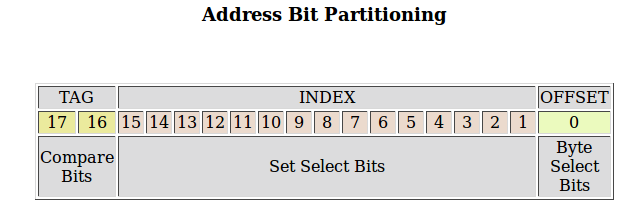
\includegraphics[scale=0.7]{figures/img/direct-abp.png}
   \caption{Address Bit Partitioning - Direct Mapped Cache.}
\label{abp-direct}
\end{figure}




\textbf{Example:} - \textit{4-way Set-Associative}
Consider the following example of a 4-way associatively mapped cache as shown in Figure \ref{set-abp} with the following parameters.

Memory size = $256KB = 2^{18}: $
Block size = $2 Bytes = 2^1$

\textit{Number of sets in cache = Cache size/(Set size * Block size) \\
\hspace*{5em}
 $64KB$/$(4  blocks * 2B)$ =
$2^{16}/(2^2 * 2^1) = 2^{13}$}

\textit{Number of bits in Tag = Total bits - Index bits - Offset bits = $18-13-1 = 4$}


\begin{figure}[tb!]

 %\centering
  %\captionsetup{justification=centering}    
   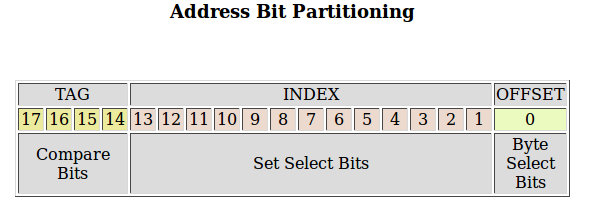
\includegraphics[scale=0.7]{figures/img/set-abp.png}
   \caption{Address Bit Partitioning - Set-Associative Cache.}
\label{set-abp}
\end{figure}

\subsection{Cache Mapping Scheme}

There are three popular methods for mapping data in a cache memory.
\begin{itemize}

\item{\textit{Direct-Mapped Cache:}  Data at a given address must be placed at a single specific location in the cache}


\item{\textit{Set-Associative Cache:} Data at a given address can be placed at any of a small set of cache locations}
 
 
\item{\textit{Fully-Associative Cache:} Data at a given address can be placed anywhere in the cache}
 \end{itemize}
 
\subsection{Direct Mapped Cache}
The direct-mapped cache is the simplest form of cache to implement. There is only one possible position  for any memory location can be cached. There is no need to search the entire cache either the particular line contains the data or not. Unfortunately, the direct -mapped cache also has the worst performance, because again there is only one place that any address can be stored which causes contention problem frequently. 


\subsection{Fully Associative Cache}


The fully-associative cache has the best cache hit ratio among all types of caches, because in a fully-associative cache, one cache line can hold any address. This means that the contention problem seen in the direct-mapped cache disappears as there is no dedicated single cache line that an address must use. However, the fully-associative cache suffers from problems involving searching the cache line. For example, if a cache consists of 16,384 lines, finding a particular address line is a computationally expensive task. Even with specialized hardware to do the searching, a performance penalty is incurred. And, this penalty occurs for all accesses to memory, whether a cache hit occurs or not. It needs more logic to determine which cache line to use when a new entry must be added (usually some form of a replacement  algorithm is employed to decide which cache line to use next). As cache address line number increases, it incurrs overhead drastically in terms of cost, complexity, and execution-time.

\subsection{Set Associative Cache}
The set-associative cache is a good compromise between the direct-mapped and fully- associative caches. Consider the example of a 4-way set-associative cache. Each address can be cached in any of four sets, and each particular set acts as a direct-mapped cache and, and within the set find the appropriate cache-line (which is like the fully associative scheme). 

\subsection{Comparison}
\begin{itemize}


\item {The fully-associative cache mapping works the best, but it is complex to implement. Each tag line needs to be compared with the desired  address tag field by the circuitry, which makes it very complex and expensive.}



\item{The direct-mapped cache has the lowest performance, but it is the easiest to implement. It is often used for an instruction cache.}

\item{The set-associative cache is a compromise between direct-mapped and fully-associative caches. The bigger the "sets" the  better the performance, but the more  complex and expensive.}

\end{itemize}

\section{Randomized Cache}
Random caches are often used to make processing systems more predictable,
such as the ARM Cortex series~\cite{ARM}.
In this work, we used a random cache model that makes programs analyzable
with MBPTA. The cache is developed in VHDL. The source code is available at~\cite{MISTLAB} and it is
configurable through generics: such as data and address bus
widths, line size, cache line count, associativity, placement/replacement, and write policy. 


The random replacement policy randomly selects the cache line to evict and make a room for the new memory address. This technique does not require to keep any information about the access history. Due to its simplicity, it has been used to analyse the system with PTA techniques. This technique also ensures that a) evictions across cache lines are independent b) the probabilities of evictions across cache lines are the same. For example, we have a \textit{W-way} set-associative cache, the probability of any specific cache line to be evicted is $\frac{1}{W}$.  Similarly, for the random placement policy, we have to ensure that the cache set in which a cache line is mapped is randomly selected. For example, assume that we have a cache with \textit{S} sets. Then the probability of a particular cache set to be selected is $\frac{1}{S}$.


\section{Cache Model}

We developed our cache model in VHDL. The cache VHDL model is configurable. The cache model can be used with different data, address, and  bus widths. The cache model can also be designed to integrate with different memory widths. There are  configurable parameters which are used to make caches with different configurations. These configurable parameters are \textit{cache line size, cache size, associativity, replacement policy, and write policy}. All parameters can be set through VHDL generics. The placement policy we used is random placement policy. We used two replacement policies: \textit{LRU} and \textit {random replacement} policies. The model supports \textit{write-through} and \textit{write-back} policies for data write. For cache misses, the cache model supports \textit{write-allocate} and \textit{no write-allocate}. In these order: we have \textit{write-back} with \textit {write-allocate}, \textit{write-through} with \textit{write-allocate}  and \textit{write through} with \textit{no write-allocate}. The maximum associativity the design can adopt is \textit{eight way}. It can be modified for more associativity, but increasing associativity increases the power and energy consumption of the system. Therefore it is highly recommended to use an associativity between four and eight. In this work, we have
used the following approach for the cache behavior
\begin{enumerate}
\item The cache uses a random replacement policy.
\item The cache uses a parametric random placement policy based on
 a hash function. The detailed design of the hash function given in Section~\ref{PHF}.
\item The cache placement is deterministic for each benchmark execution, but
  randomized across executions.
\item We measure end-to-end execution-times for a series of benchmarks.
\end{enumerate}



\subsection{Instruction Cache Model}
In this section, instruction cache, data cache, and basic state transitions are presented. The cache model is developed in Mealy state machine. To avoid fake bits, all the bits are set to zero when the cache powers up. The controller needs to clear all valid bits of indexes during the flush time and the processor is in \textbf{Flush} state, as shown in Figure~\ref{fig:inst_cache_state}.

\begin{figure}[tb!]
 %\centering
  %\captionsetup{justification=centering}    
   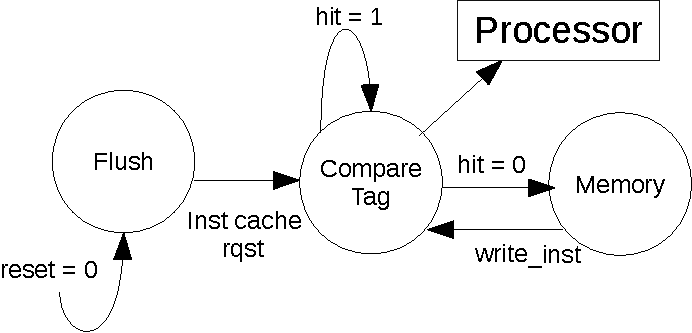
\includegraphics[scale=1]{figures/img/inst_cache_state.pdf}
   \caption{Instruction Cache State Machine.}
\label{fig:inst_cache_state}
\end{figure}

After initializing the initial states, the controller is set to the \textbf{Compare Tag} state. In this state, the controller needs to verify the tag of the instruction. The requested instruction from the processor either resides in the cache or not. If the requested instruction resides in the cache, a cache \textbf{hit} occurs and the instruction is delivered to the processor. If the requested instruction is unavailable, a \textit{miss} occurs and the controller state changes to the \textbf{Memory} state. In this state, the cache needs to load a whole memory block into the cache line which contains the requested instruction. Then the state machine goes back to \textbf{Compare Tag} state. At this stage, the cache replacement policy works to replace cache lines.

\subsection{Data Cache Model}

Our data cache controller used the \textit{write-back policy}. The flushing operation remains the same as for the instruction cache. Data cache remains in the \textbf{Idle} state and works only when it receives the request from the processor. Because data access requests from the processor are less than the instruction requests, it is better to keep data cache in \textbf{Idle} state and wait for the processor request. When the processor requests for reading or writing the data, the controller changes its state. For both requests, the controller checks if the data is in the cache or not. Suppose that the requested data is not available and the victim cache
 line is dirty. This means that the data cache line selected by the replacement policy is not in the memory (no copy in the memory). In this case, data is written back to the main memory. Then the requested data is copied from the main memory, put in the victim cache line (update cache) and processor reads the newly updated cache line. Figure~\ref{fig:data_cache_state} shows the data cache state machine. 




 \begin{figure}[tb!]
% \centering
 % \captionsetup{justification=centering}    
   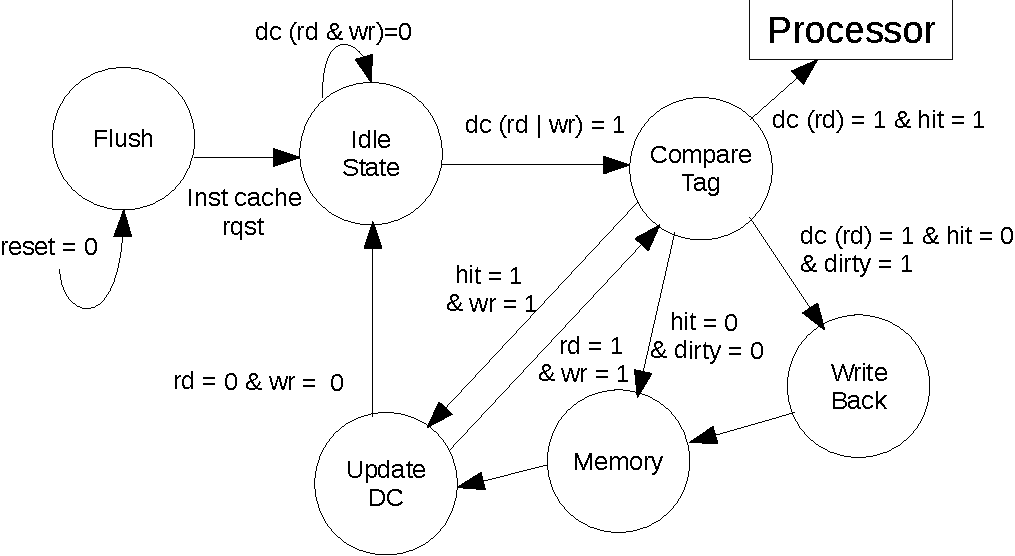
\includegraphics[scale=0.8]{figures/img/data_cache_state.pdf}
   \caption{Data Cache State Machine.}
\label{fig:data_cache_state}
\end{figure}




\begin{table}[tb!]
\center
\caption{VHDL Basic Signals Descriptions.}


\begin{tabular}{|c | c|} 
 
 \hline
Record  & Signal Description  \\ 
\hline

 
 
 ic\_in.addr & instruction cache address  \\
 ic\_in.stall & stall the instruction cache  \\ 
 \hline
 
 in\_out.data & instruction from cache \\
 dc\_in.addr & request data address\\
 dc\_in.data & write data on write request \\
 dc\_in.mask & mask write \\
 dc\_in.rd &  request for read \\
 dc\_in.wr & request for write \\
 \hline

 dc\_out.data & return data from cache \\
 dc\_out.stall & stall data cache \\
 mem\_in.data & data from main memory \\
 mem\_in.stall & stall main memory \\
 \hline
 mem\_out.addr & address to requested data\\
 mem\_out.data & on write request write data\\
 mem\_out.mask & mask write\\
 mem\_out.rd & request for read\\
 mem\_out.wr & request for write\\
 
 \hline
 
 

\end{tabular}
\end{table}

\section{Hardware Implementation}
\label{Hardware Implementation}  
\subsection{Cache RTL Model}
\label{Cache Model}

We implemented instruction and data caches for the Ion
MIPS32 processor~\cite{ION}. A completely novel, configurable cache
design was implemented in VHDL and integrated with the Ion core. The
cache is completely configurable (bus width, size, block size,
policies, etc.) with VHDL generics and could be easily ported to other
processor designs. Figure~\ref{fig:cache-structure} shows the main components of our design:

\begin{figure}[tb!]
% \centering
 % \captionsetup{justification=centering}    
   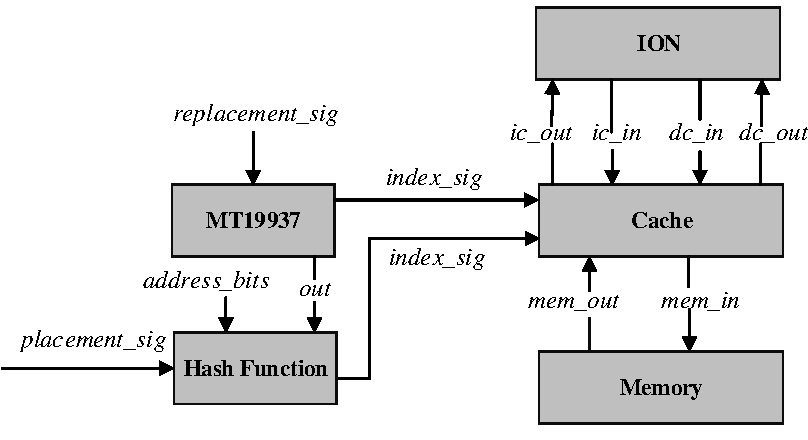
\includegraphics[scale=1]{figures/img/cache_structure_c.pdf}
   \caption{Structure of the Proposed Cache.}
\label{fig:cache-structure}
\end{figure}

\begin{enumerate}
\item The cache block contains the memory elements, as well as the
logic to manage the placement policy (modulo) and replacement policies (random and least-recently-used).
\item A hash function block that operates on the index signal to the
  cache, randomizing the mapping between memory blocks and cache blocks.
\item A pseudo-random number generator (MT19937).
\item The Ion core, which provides a MIPS32 ISA and controls the whole
  system.
\end{enumerate}

Our cache has three fundamentally novel features that enable probabilistic
timing analysis:
\begin{enumerate}
\item A random \textbf{placement} policy which uses a parametric hash
  function to shuffle the initial placement of blocks in the cache memory.
\item A random \textbf{replacement} policy that uses high-quality random
numbers to provide statistically-verifiable guarantees that replacement
events are uniformly distributed among the available cache blocks.
\item A high-quality pseudo-random number generation, with an extremely
long period, to generate random bits for the implementation of the cache
random policies.
\end{enumerate}
%
%
\subsection{Random Number Generation}

In our cache design, we used the Mersenne Twister algorithm to
generate random numbers. In particular, we used the MT19937 algorithm,
which is considered as a good hardware solution for a random number
generation~\cite{Matsumoto:1998:MTE:272991.272995}. MT19937 provides a
uniform pseudo number pattern with a period of
$2\textsuperscript{19937-1}$, and a width of 32 or 54 bits.  We used
the OpenCores implementation of MT19937~\cite{OpenCores}. The
synthesis report shows that the maximum clock frequency the design can
achieved is 147.016 MHz, with a throughput of 30 Megasamples per second.
%\subsection{Implementation Details}

\subsection{Parametric Hash Function}
\label{PHF}

\begin{figure}[tb]

% \centering
 % \captionsetup{justification=centering}    
   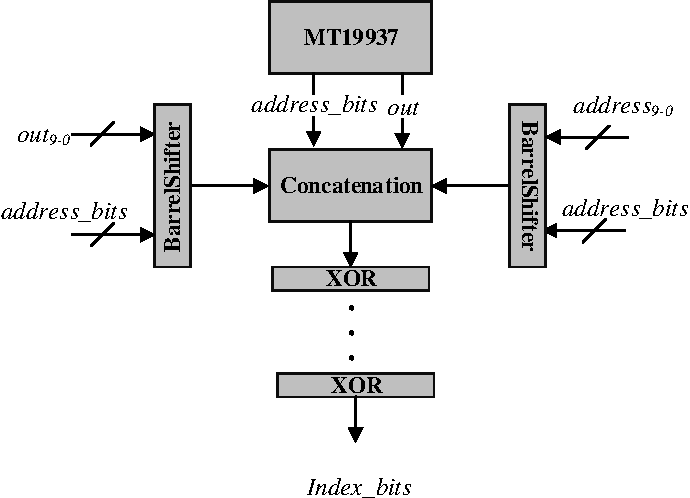
\includegraphics[scale=1]{figures/img/hash_function.pdf}
   \caption{The Hash Function uses a Random Number, the Address Bits, and Four XOR Stages to Produce a Random Placement.}
\label{fig:hash_function}
\end{figure}


The idea of using a parametric hash function (PHF) is proposed by~\cite{Kosmidis:2013:CDP:2485288.2485416}. The purpose of using a parametric hash function is to get the index bits for random placement in a cache. The implementation for a parametric hash function is shown in Figure~\ref{fig:hash_function}.
This design is remodelled
for this work, replacing their Multiply With Carry (MWC) random number
generator with the MT19937, which increases the quality of the random
numbers as well as the period.  The redesign was driven by the fact
that MWC does not pass some statistical normality
tests~\cite{bandyopadhyay2015discrete}, and its period might be
insufficient for long running
applications~\cite{Goresky:2003:EMR:945511.945514}.

Standard placement assigns cache sets to memory addresses based on the index bits. If the placement policy assigns two memory
addresses to the same cache set, they will systematically be in conflict. 
To deal with this deterministic nature, we randomized the timing
behavior of the placement policy. To achieve this, we used a parametric hash
function with a random number as an input.  A random number
provides a unique and constant cache set mapping for each address.


If the random number changes, the cache set to which the address is mapped changes. By changing random number only at a new execution, programs can be analyzed with end-to-end runs assuming that the cache is initially empty. The hash function is used to get the~\textit{$index\_bits$}. Then these \textit{$index\_bits$} are used for cache placement. The hash function has two inputs 1) the \textit{$address\_bits$} 2) the output from random number generator signal \textit{out}, as shown in Figure~\ref{fig:hash_function}. 



The hash function uses the barrel shifter which rotates the address bits based on the randomly generated bits from MT19937 block (random number generator block).  Assumed 32-bit addresses the \textit{$address\_bits$} signal in Figure \ref{fig:hash_function} needs 27 bits as 5 offsets bits were discarded. Similarly, the other block of barrel shifter uses some of its own bits to shift the original address bits. By doing this, we want to ensure that for different random numbers the mapping of that address changes (data mapped from memory to cache on different locations). This operation is done by the rightmost barrel shifter. Finally, all the original address bits, rotated address bits and bits rotated by random number generator out signal are concatenated and XORed successively till we get desired \textit{$index\_bits$}.








\section{Experimental Results}


We present the RTL model of randomized L1 data and
instruction caches. The caches use a high-quality random number
generator for random placement and replacement. Random placement is
obtained with a parametric hash function that shuffles the association
between memory addresses and cache blocks. The cache is integrated
with the Ion MIPS32 processor, and verified to generate independent
and identically distributed timing events, to apply MBPTA technique. 
We test our cache
and MBPTA approach on a variety of benchmarks from the M\"alardalen
benchmark suite and show a noticeable improvement (5-15\%) in terms of
measured Worst Case Execution Time as well as enabling the
identification of safe probabilistic WCET bounds. Table~\ref{det/pro} and Table~\ref{pvsd} show the prediction bounds obtained by applying MBPTA on the probabilistic cache, and  also show the estimates obtained for the deterministic cache (\textit{modulo placement and LRU replacement}) under the  deterministic timing technique named \textit{reuse-distance}~\cite{beyls2001reuse}. For example in Figure~\ref{application:crc} shows the pessimism between the probabilistic architecture and deterministic architecture for the application \textbf{crc}. Here, we observe that the probabilistic architecture provides less pessimism than the deterministic one as probabilistic architecture has less dependency on the execution history and required no knowledge of the hardware architecture.





\begin{figure}[tb!]
 %\centering
  %\captionsetup{justification=centering}    
   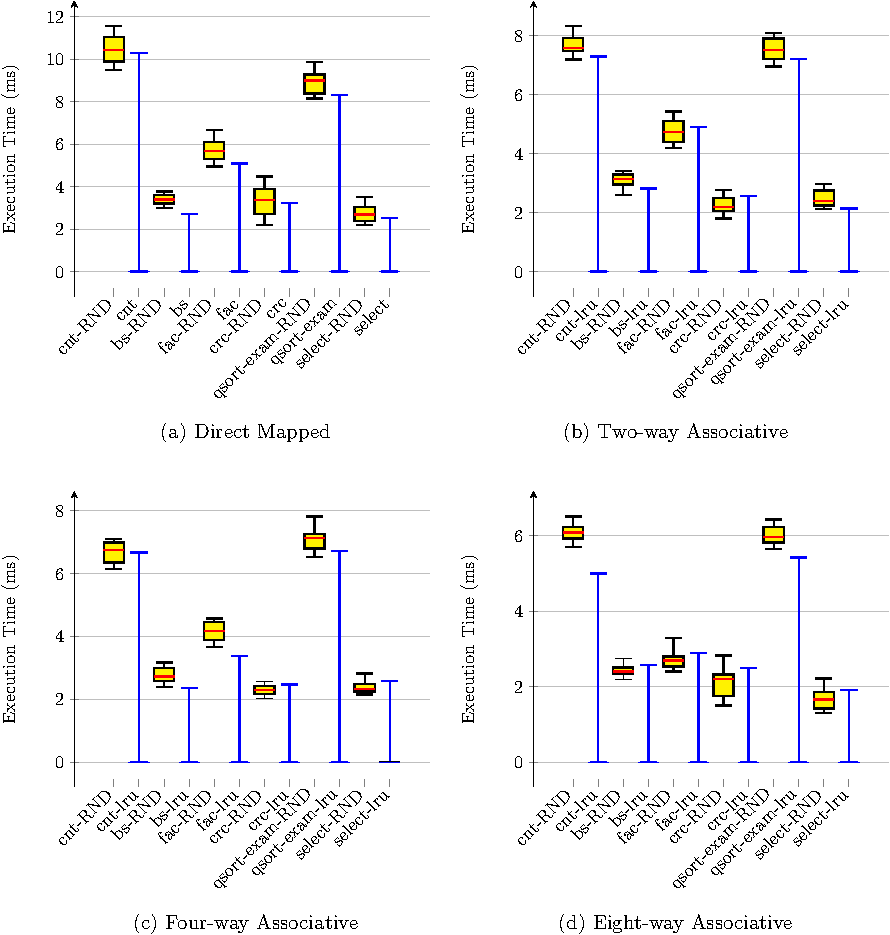
\includegraphics[scale=1.1]{figures/img/boxplot.pdf}
   \caption{Execution-Time Measurement.}
\label{fig:boxplot}
\end{figure}



\begin{table}[t]

\caption{Resource Utilization and Overhead (Virtex-5).}
\scalebox{0.9}{
\label{resource}
\begin{tabular}{ccccccc}
\toprule

              & Available & Deterministic & Probabilistic & \color{red}{Hash} & \color{red}{Random} & Overhead (\%) \\
              & \multicolumn{1}{c}{resources} 
               & \multicolumn{1}{c}{cache} 
                & \multicolumn{1}{c}{cache} 
                 & \multicolumn{1}{c}{\color{red}{function}} 
                  & \multicolumn{1}{c}{\color{red}{generator}} \\
                \bottomrule   
%\cmidrule(lr){3-5}
%              &   &  Cache & Hash	& MT19937 &  \\
%\midrule
%%Available     & 69120    &       69120   & 69120       
%LUT Flip Flop  & 1904    &  1792   &  656   &  117  & 34.7    \\
LUT Flip Flop  & 17708    &  1904   & 1792    &  656  & 117 & 4.36\% \\ 
Slice LUTs     & 69120    &   6026  &   5637  &  660  &419 & 1.56 \%  \\
%%BRAMs          & 4       &  6      &  2     &  1    & 225\%\\
\bottomrule
\end{tabular}
}

\end{table}





%\begin{table}[t]
%\caption{Resource Utilization and Overhead (Virtex-5)}
%\label{resource_table}
%\begin{center}
%\begin{tabular}{llllll}
%\toprule
%              & LRU & \multicolumn{3}{c}{RND} & Overhead \\
%\cmidrule(lr){3-5}
%              &   &  Cache & Hash	& MT19937 &  \\
%\midrule
%%Available     & 69120    &       69120   & 69120           \\
%LUT Flip Flop  & 1904    &  1792   &  656   &  117  & 34.7\% \\ 
%Slice LUTs     & 6026    &  5637   &  660   &  419  & 11.6\%  \\
%%BRAMs          & 4       &  6      &  2     &  1    & 225\%\\
%\bottomrule
%\end{tabular}
%\end{center}
%\end{table}



\subsection{Achieving i.i.d Property}

We used random placement and random replacement policies with the guarantee that observed execution-times fulfill the property of MBPTA that is essential to apply probabilistic technique.  In order to test independence we used Wald-Wolfowitz independence test~\cite{gumbel1954statistical}. We used a 5\% significance level, a typical value for these types of tests~\cite{Kosmidis:2013:CDP:2485288.2485416}. The independence test gets successful if the obtained absolute values are lower than $1.96$, and higher otherwise~\cite{Kosmidis:2013:CDP:2485288.2485416}.
Table~\ref{itest} shows the independent tests results.

 We used Kolmogorov-Smirnov ~\cite{gumbel1954statistical} test to verify the observed execution-times  are identically distributed. The significance threshold set for this test is $0.05$. If the test values are above the significance level, the result is considered pass, and fail otherwise. Table~\ref{id test} shows the independent distribution tests results.





\begin{table}
\center
\caption{Independence Tests.}

\label{itest}



\begin{tabular}{|c | c| c | c| c| c |} 
 \hline
Benchmark & DM & 2-way SA & 4-way SA & 8-way SA  \\ 
\hline

 
 
 cnt & 0.82 & 0.87 & 0.63&  0.07 \\
 \hline
 bs & 0.51 & 0.75 & 0.11& 0.23\\ 
 \hline
 
 fac & 0.33 & 0.76  & 0.44 & 0.53\\
 \hline
 crc & 0.17 & 0.27 & 0.37& 0.51\\
 \hline
 qsort-exam & 1.26  &0.41 & 0.33 & 0.03\\
 \hline
 select & 0.39 &1.24 &0.63 &1.12 \\
 \hline
 
 
\end{tabular}

\end{table}

\begin{table}
\center
\caption{Identical Distribution Tests.}

\label{id test}

\begin{tabular}{|c | c| c | c| c| c |} 
 \hline
Benchmark & DM & 2-way SA & 4-way SA & 8-way SA  \\ 
\hline

 
 
 cnt & 0.43 &0.65 & 0.28&0.54  \\
 \hline
 bs & 0.97 & 0.70&0.34 &0.36 \\ 
 \hline
 
 fac & 0.81 & 0.39 &0.74 &0.28 \\
 \hline
 crc & 0.48 & 0.40 & 0.12&0.96 \\
 \hline
 qsort-exam & 0.39  &0.93 &0.73  &0.54 \\
 \hline
 select & 0.35 &0.93 &0.41 &0.28 \\
 \hline
 
 
\end{tabular}
\end{table}



The architecture used in our experiments is the OpenCores Ion MIPS32
processor. We integrated instruction and data caches, and we
implemented the whole system on the Xilinx ML505 FPGA evaluation
board, using the XC5VLX110T chip,  Xilinx ISE-14.4 and ModelSim 10.1.a. We used two separate 4-KB cache
memories for data and instructions, both with a 32-byte line size.  To
evaluate our design, we used M\"alardalen real-time benchmark~\cite{mrtc:bench} suite. We selected six benchmarks: \textit{cnt, bs,
  fac, crc, qsort-exam} and \textit{select}. These benchmarks use arrays
and matrices, and have nested loops structures which are ideal to test
our design~\cite{Competitive}. We omitted those benchmarks using
external libraries and unstructured code to simplify the
software implementation and data collection. 



Each benchmark is run on multiple cache configurations profiles, and derived its execution-time profile using MBPTA, with 1000 runs per
profile to approximate a normal  distribution.
%To show that our cache generates identically distributed execution-times (as
%required for PTA), we used the Kolmogorov-Smirnov test~\cite{books/daglib/0020904},
%which shows that the null hypothesis (the data are normally distributed) cannot
%be rejected for all benchmarks at the 5\% confidence level ($p>0.062$).
We compared our results (RND) with a standard Least-Recently-Used (LRU)
cache policy implementation. Table~\ref{resource} shows the resource utilization and overhead of the probabilistic cache, the main source of overhead are due the extra logic consumed by the hash function and random number generator, but the overhead we observed is negligible as compared with the resources available on the Virtex-5. This design gives freedom that we can integrate different IP-cores and other functionalities in our design. Starting from the direct-mapped cache with random placement, we observed the execution-time taken by the benchmarks is more than that by the set-associative cache. This is due to the fact that if we increase the associativity, the number of cache misses are reduced and it helps to increase the execution-time. Increasing the associativity also helps to improve the prediction as the execution-time getting decrease also helps to smoothing the uniform distribution of the execution-times as a result obtained trustworthy and tight estimates. Figures \ref{fig:boxplot} shows the timing
distributions for all benchmarks on our cache from direct-mapped to
8-way associative, respectively. As an added advantage, our random
cache shows a 19\% improvement in worst case execution-time w.r.t to
a direct-mapped cache, 11\% for 2-way cache, 8\% for a 4-way
cache, and 6\% for an 8-way cache. As expected, LRU gets closer to RND
as the number of ways increases: the number of conflict misses is
greatly reduced by additional ways.


%\begin{table}[tb!]
%  \caption{Predicted pWCET ($T_p$) at $10^{-3}$ Exceedance Probability versus Measured WCET ($T_m$) for the RND cache. Times are shown in milliseconds.}
%\label{pWCETTiming}
%\centering
%\begin{tabular}{lllllllll}
%\toprule
%Benchmark & \multicolumn{2}{l}{Direct} & \multicolumn{2}{l}{2-way} & \multicolumn{2}{l}{4-way} & \multicolumn{2}{l}{8-way}    \\
%\cmidrule(lr){2-3} \cmidrule(lr){4-5} \cmidrule(lr){6-7} \cmidrule(lr){8-9}  
%                &  $T_m$ & $T_p$  &  $T_m$ & $T_p$ &  $T_m$ & $T_p$ &  $T_m$ & $T_p$ \\
%\midrule
%cnt       &  11.58 & 15.35  & 8.30 & 9.76 & 7.11 & 8.75& 6.52 & 7.90    \\ 
%bs        &  3.77  & 6.10   & 3.42 & 5.06  & 3.17 & 4.22 & 2.57 & 3.77 \\ 
%fac &  6.67  & 9.31  & 5.44 & 7.42 & 4.62 & 6.36 & 2.90 & 3.95 \\ 
%crc       &  4.49  & 7.23  & 2.50 & 5.06  & 2.77 & 4.90  & 2.50 & 4.29\\ 
%qsort-exam     &  9.98  & 12.08  & 9.10 & 11.18 & 7.83 & 10.26 & 6.43 & 8.34 \\ 
%select    &  3.80  & 5.43  & 2.98 & 4.55  & 2.59 & 3.44  & 1.99 & 3.02  \\ 
%\bottomrule
%\end{tabular}
%\end{table}

\begin{table}[tb]
  \caption{Predicted pWCET ($T_p$) at $10^{-3}$ Exceedance Probability versus Measured WCET ($T_m$) for the RND Cache. Times are shown in milliseconds.}
\label{pWCETTiming}
\centering
\begin{tabular}{lllllllll}
\toprule
Benchmark & \multicolumn{2}{l}{Direct} & \multicolumn{2}{l}{2-way} & \multicolumn{2}{l}{4-way} & \multicolumn{2}{l}{8-way}    \\
\cmidrule(lr){2-3} \cmidrule(lr){4-5} \cmidrule(lr){6-7} \cmidrule(lr){8-9}  
                &  $T_m$ & $T_p$  &  $T_m$ & $T_p$ &  $T_m$ & $T_p$ &  $T_m$ & $T_p$ \\
\midrule


cnt       & \color{red}{11.58} & \color{red}15.35  & 8.30 & 9.76 & 7.11 & 8.75& \color{red}6.52 & \color{red}7.90    \\ 

bs        &  3.77  & 6.10   & 3.42 & 5.06  & 3.17 & 4.22 & 2.75 & 3.77 \\ 
fac &  6.67  & 9.31  & 5.44 & 7.42 & 4.62 & 6.36 & 3.33 & 3.95 \\ 
crc       &  \color{red}{4.49}  & \color{red}{7.23}  & 2.50 & 5.06  & 2.77 & 4.90  & \color{red}{2.82} & \color{red}{4.29}\\ 
qsort-exam     &  9.98  & 12.08  & 9.10 & 11.18 & 7.83 & 10.26 & 6.43 & 8.34 \\ 
select    &  3.80  & 5.43  & 2.98 & 4.55  & 2.59 & 3.44  & 2.22 & 3.02  \\ 
\bottomrule
\end{tabular}
\end{table}

Moreover, we have observed the pWCET estimates obtained with the MBPTA technique as explained in Section\ref{MBT}. The MBPTA method based on the EVT on the execution runs and observed the pWCET estimates. 
Table~\ref{pWCETTiming} shows the  pWCET obtained with MBPTA
for the multiple random placement/replacement cache configurations. We
consider the pWCET estimates at the exceedance probability (the
probability that the execution-time will exceed the predicted value)
of $10^{-3}$, as this is compatible with our number of simulations
(1000 runs). The data show that the pWCET is a very tight bound for the
measured WCET. 



We observed a set-associative cache with random placement and replacement provide the tight pWCET estimates as comparing it with the LRU policy. Similarly,  we observed that the estimates provided by random policies provided much tight estimates as cache associativity increases. On average, we observed that the estimation is improved from 2-way set-associative to 8-way set-associative, e.g. the prediction time observed for the \textit{cnt} the difference between measured time and predicted time is $3.77$ ms which is reduced for the 8-way set-associative to $1.38$ ms. Table~\ref{pWCETTiming} summarizes all the \small{p}WCET. Random replacement policy has a lower probability of cache conflicts which helps to improve the execution-time and provide less pessimism in prediction under the MBPTA technique. Indeed, random placement and replacement policies provide the best hardware platform to PTA techniques to the estimates of pWCET with less pessimism.




In summary, our tests show that our random cache implementation can 
successfully provide a probabilistically analyzable cache on FPGA:  MBPTA
can be applied to provide safe bounds with arbitrary accuracy. In short, compared to deterministic cache the observed execution-time is 19\% improved
 for direct-mapped cache, 11\% improved for 2-way, 8\% and 6\%
 improvement observed for 4-way and 8-way respectively. Consider a benchmark \textbf{qsort-exam} in Table~\ref{det/pro} the prediction bound obtained under the probabilistic cache is $8.34$ ms and the prediction bound obtained under the deterministic cache is $11.09$ ms which is about $28.30$ \% more than the probabilistic cache.
 
 
 
 
 
 
 
 \begin{table}[tb!]
\caption{Deterministic/Probabilistic WCETs and respective Bounds.}
\centering
\label{det/pro}
%\hspace{2.8cm} 
\scalebox{1}{

\begin{tabular}{lcccccccc}
\toprule
Benchmark & \multicolumn{8}{c}{Execution-Time (ms)}    \\
\cmidrule(lr){2-2} \cmidrule(lr){4-4} \cmidrule(lr){6-6} \cmidrule(lr){8-8} 

& Deterministic  & & Prediction  & & Probabilistic & & Prediction \\
 &  \multicolumn{1}{l}{\hspace{0.5cm}{Cache (WCET)}} & & bound & & Cache (WCET) & & bound\\
  
 

  \midrule

 

%  \midrule
%
%
cnt       &   \multicolumn{2}{c}{5.04} & \multicolumn{2}{c}{10.33}    & \multicolumn{2}{c}{6.52} & \multicolumn{1}{c}{7.90} & \\
bs       &   \multicolumn{2}{c}{2.57} & \multicolumn{2}{c}{6.77}    & \multicolumn{2}{c}{2.75} & \multicolumn{1}{c}{3.77} \\
fac       &   \multicolumn{2}{c}{2.93} & \multicolumn{2}{c}{5.45}    & \multicolumn{2}{c}{3.33} & \multicolumn{1}{c}{3.95}\\
crc       &   \multicolumn{2}{c}{2.50} & \multicolumn{2}{c}{6.13}    & \multicolumn{2}{c}{2.82} & \multicolumn{1}{c}{4.29} \\
qsort-exam       &   \multicolumn{2}{c}{5.43} & \multicolumn{2}{c}{11.09}    & \multicolumn{2}{c}{6.43} & \multicolumn{1}{c}{8.34} \\
select       &   \multicolumn{2}{c}{3.91} & \multicolumn{2}{c}{5.34}    & \multicolumn{2}{c}{4.12} & \multicolumn{1}{c}{5.18}
\\
\bottomrule
\end{tabular}
}
\end{table}
 
  
 
 
 
 
 
 
 
 
 
 
 
\begin{table}[tb!]
\caption{Pessimism between Predicted pWCETs at $10^{-3}$ Exceedance Probability versus Deterministic Cache.}
\centering
\label{pvsd}
\scalebox{1.2}{

\begin{tabular}{lcccccc}
\toprule
 & \multicolumn{6}{c}{Pessimism Difference(\%)}   \\
\cmidrule(lr){2-2} \cmidrule(lr){3-3} \cmidrule(lr){2-2} \cmidrule(lr){4-4}\cmidrule(lr){5-5} \cmidrule(lr){6-6} \cmidrule(lr){7-7}


  
 & cnt     & bs   & fac  & crc &  qsort &  select  \\


  \midrule

Deterministic cache       &   \multicolumn{1}{c}{68.83} &

 \multicolumn{1}{c}{89.93}  & \multicolumn{1}{c}{60.14}&\multicolumn{1}{c}{84.12}
  &   \multicolumn{1}{c}{68.52} &   \multicolumn{1}{c}{30.91}   \\
 
Probabilistic cache       &   \multicolumn{1}{c}{19.14} &

 \multicolumn{1}{c}{31.28}  & \multicolumn{1}{c}{17.033}&\multicolumn{1}{c}{41.35}
  &   \multicolumn{1}{c}{25.86} &   \multicolumn{1}{c}{22.79}   \\


\bottomrule
\end{tabular}
}
\end{table}
 
 
 
  The improvement
 factor for higher associativity is not much higher because for the deterministic cache (modulo placement and LRU replacement)  policies
 also works quite good as associativity increases, which decreases the room for
 further improvement. Table~\ref{det/pro} and Table~\ref{pvsd} shows the pWCET
 estimates obtained with MBPTA for the probabilistic cache that reduces the pWCET estimates over deterministic cache (\textit{modulo placement and LRU replacement}) analyzed with DTA technique~\cite{beyls2001reuse}.
 These measurements give us confidence for WCET bounds. The WCET
 analysis gives a safe and trustworthy bound, and this bound may be
 less conservative as compared it with the bounds obtained for the deterministic cache with deterministic timing technique. Furthermore, the WCET gives no general guarantee that we
 have knowledge about the worse-case path. The measured WCET gives an
 upper bound of the pessimism of the WCET analysis. In this work we
 provide a real execution-time profile on probabilistic cache which is generally not as much over
 estimated as we seen in 
 Table~\ref{det/pro}. The difference between the deterministic cache execution-time and its associated prediction bounds is more pessimistic than the difference between the probabilistic cache execution-time and its associated prediction bounds. 
 
 
 
 









In this work, we make it possible to use
 a probabilistic approach in an FPGA's. This work also helps to make it possible to use probabilistic timing technique in real-time systems.
\begin{figure}[h]
 %\centering
  %\captionsetup{justification=centering}    
   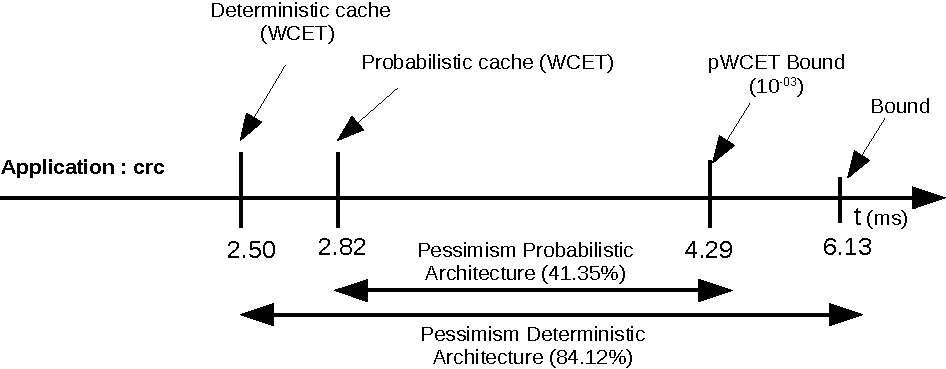
\includegraphics[scale=0.8]{figures/tpc-example1.pdf}
  \caption{Pessimism between Predicted pWCETs at $10^{-3}$ Exceedance Probability versus Deterministic Cache.}
\label{application:crc}
\end{figure}



















\section{CACHE DESIGN CONSIDERATIONS TO IMPROVE TIMING ANALYSIS BOUNDS}





In this chapter, we discuss the comparison between probabilistic timing analysis techniques --- SPTA and MBPTA --- for time- prediction estimates.  We also discuss how we modified the LEON-3
processor's caches to make it applicable for the probabilistic timing techniques.  We use random placement and replacement policies for caches and applied probabilistic timing analysis techniques under varying
cache configurations to measure the pessimism associated with each cache configuration. The purpose of this work is to find the time- prediction estimates with measurements done
on the processor to help real-time system designer to
evaluate the level of pessimism for different  cache architectures
using  probabilistic timing analysis techniques. We also identified the strengths and limitations of each technique for time-
prediction that helps designers to design the processor's architecture to observe the level of pessimism that is associated with the timing analysis techniques.


\section{Introduction}
\label{intro}

As discussed in Chapter\ref{sec:paper1}, we used the same strategy --- hash function and random number generator --- for cache randomization. We used randomization for cache placement and replacement policies.  The PTA techniques are used to provide probabilistic WCET estimates for arbitrarily low probabilities. The estimates and level of pessimism offered by the PTA techniques are less pessimistic than those by the deterministic timing techniques~\cite{abella2014comparison}. We measured pWCET estimates  with both variants of PTA --- SPTA and MBPTA. This work is mainly focused on the study of pessimism under different cache configurations while applying PTA techniques. We studied and discussed which technique offered less pessimism, how these techniques are useful for the time-prediction under varying cache configuration and how pessimism varies under different cache configurations. We also compared the PTA techniques with the timing values obtained from the deterministic architecture in which a randomized cache is replaced with a ~\textit{Least-recently used (LRU)} cache. However, both approaches need specific hardware and software conditions~\cite{abella2014comparison}. For instance, DTA techniques perform better on a deterministic architecture with time-deterministic caches (Least Recently Used replacement policy), whereas, PTA techniques performed better on a time-randomized architecture~\cite{abella2014comparison,anwar2015probabilistically}. 
\newline
The contributions of this work are:

\begin{itemize}

\item{In this work, we focused on the time predictability under different cache choices. We have applied PTA techniques (MBPTA and SPTA) on the M{\"a}lardalen benchmark~\cite{mrtc:bench}. We identified the limits and strengths of both methods that show pessimism varies under varying cache parameters on the randomized hardware equiped with the time-randomized cache~\cite{anwar2015probabilistically}}.

\item{We studied the prediction on a randomized hardware. We also discussed the predictability with cache enabled with a deterministic approach, i.e. a time-deterministic cache, e.g.~\textit{LRU}}.

\item{The hardware and software environment remain the same for both timing techniques. We also compared the estimated WCET with the that from a deterministic approach}. \item{We  varied the sensitivity of the cache parameters, e.g. \textit{associativity, cache line size, and cache size}}.

\item{Our work allows the cache designer to appropriately select the
cache parameters to obtain the predictability goals by
probabilistic timing analysis techniques}.
\end{itemize}

 


\section{WCET Estimation Techniques}
\label{WET}
\subsection{Cache Overview}

The cache contents can be organized in different ways.  Each design is  part of processor's architecture and have different power, timing, and functionality characteristics. The most common cache configurations are \textit{a) direct-mapped cache, b) fully-associative cache,} and  \textit{c) set-associative cache}. The direct-mapped cache has a unique address for each stored data. Usually, modulo function is used as a placement function. On the other hand, the fully-associative cache does not use any placement function. Data from main memory can be stored in any physical cache line. Therefore, a fully-associative cache requires only replacement function to decide which cache line to evict. The LRU and random policies are usually used as a replacement function for a fully-associative cache. The last one is the set-associative cache which is a combination of direct and fully-associative caches. The number of sets in a cache is decided by the direct-mapped scheme and in each set the cache lines is determined by fully-associative scheme. Therefore, a set- associative cache has to implement both random placement and  replacement policies.  In this work, we have used set-associative caches. 
\section{Timing Techniques}
\subsection{Deterministic Timing Analysis}
\label{timing techniques}
DTA techniques need a cycle-accurate model of the system and mathematical representation of the code to obtain the safe upper bound for the worst execution-time~\cite{wilhelm2008worst}. As discussed in Chapter~\ref{sec:intro}, advancements in the architectural features and adoption of more complex systems lead to the \textit {timing analysis wall} that limits the usage of  deterministic timing techniques~\cite{zhou:spta}. The DTA techniques are divided into two sub-categories named as \textit{low-level analysis} and \textit{high-level analysis} techniques. The \textit{low-level analysis} techniques use the model of a processor architecture and \textit{high-level analysis} techniques identify the longest execution path among all possible flows of the program for multi-path program analysis. The DTA techniques are applied at cache level, enabled with LRU replacement policy. For timing analysis, this technique needs a knowledge of all previous memory accesses made by the program. This requires an accurate abstract cache model. Any flaw in that model, (e.g. addresses of some memory accesses are unknown) provides degradation of the WCET estimation. But in some cases, where required hardware and software detailed knowledge are available, DTA techniques provide the tightest WCET estimations. In this work, we did not use any specific DTA technique as this approach is out of the context of this work rather we used deterministic architecture (LRU-cache) to obtained the execution bound. The execution bound obtained from the deterministic architecture is enough to show that the level of pessimism is significantly high.



This section provides the overview of the timing analysis techniques that we used for the time-prediction analysis.

\subsection{Measurement-Based Probabilistic Timing Analysis}
\label{mbpta}
MBPTA is a technique used to reduce the cost of acquiring the knowledge needed for computing trustworthy WCET bounds~\cite{cucu2012measurement,kosmidis2014pub}. MBPTA seeks to determine the WCET estimates for arbitrarily low probabilities of exceedance, namely probabilistic WCET (pWCET). This technique is based on the Extreme Value Theory (EVT) and provides an estimation of the WCET of a task or application running on a hardware platform. In order to defeat the dependence on the execution history, this technique employs randomization. Therefore, MBPTA technique uses the theory of rare events~\cite{Cazorla:2013:PPA:2465787.2465796}. There are two rare event theories that fit the WCET estimation: \textit{theory of extreme values}~\cite{gumbel1954statistical} and \textit{theory of large deviations}~\cite{gumbel1954statistical}. To the best of our knowledge, EVT is the only implemented theory for WCET estimation so far. EVT provides an estimation for the maximum of a sequence of i.i.d random variables~\cite{hoeffding1963probability}. In this work, we have used the MBPTA technique that allows us to find the predicted time of the programs. We have obtained the pWCET estimations that can be applied with high confidence as an upper bound on the execution-time. The execution-times of the programs are observed for 1,000 times (runs). If those execution-times can be modeled with i.i.d random variables, then the pWCET of a program can be obtained by constructing an Empirical Cumulative Distribution Function (ECDF). As we are interested in the EVT and this theory is used to estimate the probability of occurrence of extremely large values that are  \textit{rare events}. EVT estimates the distribution function for either the maximal or  the minimal values from \textit{n} set of observations which are formed with the random variables. In short, EVT is used to estimate the extremes. 
\subsection{Modelling EVT for WCET}

In order to model  EVT for WCET estimates, consider an example of \textit{i.i.d} random variables $\left \{ X_1,X_2,...,X_n \right \}$. Let $M_n$  be the maximum value defined as $M_n = max \left \{ X_1,X_2,...,X_n \right \}$. Consider \textit{F} as distribution function and there exits real number sequence $(a_n,b_n)$ such that $a_n > 0$ and $\lim_{n \to \infty}  P (\frac{M_n-b_n}{a_n}\leq x) = F(x)$. Then \textit{F} belongs to either the \textit{Gumbel}, the \textit{Frechet}, or the \textit{Weibull} family~\cite{gnedenko1943distribution}. The function \textit{F} denotes the distribution function of random variables. In our case, the random variables are used to construct the execution-times of the programs. We observed that the execution-times of the programs follow this property by applying the Kolmogorov-Smirnov test~\cite{KS-test} for identical distribution test and Wald-Wolfowitz~\cite{gumbel1954statistical} for independence test. Table~\ref{iid-2-test} shows the values obtained by applying these two tests. We used the distribution to model the Cumulative Distribution Function (CDF) which has the following form:


$$F_\xi (x) = \left\{\begin{matrix}
e^{-(1+\xi \frac{x-\mu}{\sigma }^\frac{1}{\xi})}& \xi \neq 0\\ 
   
    e^{-e}\strut^{-\frac{x-\mu}{\sigma}}
                                  & \xi = 0 
\end{matrix}\right.$$


This equation is called Generalized Extreme Value distribution and is defined by three parameters:
a) shape ($\xi$), b) scale ($\sigma$), and c) location ($\mu$). We need to estimate these three paramters in order to find the sequence of real number $(a_n,b_n)$.
For Gumbel distribution, we used shape parameter ($\xi=0$).
\begin{table}
\center
\caption{Independence and Identical Distribution Tests.}

\label{iid-2-test}

\begin{tabular}{|c | c| c | c| c| c |c |c |} 
 \hline
ud & cover & expint & fdct &jfdctint&qsort&select&cnt  \\ 


\hline

 
 %<1.96
 
 \multicolumn{8}{c}{Independence Test} \\
 \hline 

 
 0.81 & 0.92  & 0.84 & 0.67&0.77 &0.69 &0.85 &0.93   \\
 \hline
 %>0.05
 \multicolumn{8}{c}{Identical distribution Test} \\
 \hline
 0.24&0.38  &0.91 &0.69&0.92 &0.87 &0.56 &0.40   \\
 \hline
 
 
\end{tabular}
\end{table}

\subsection{Steps in MBPTA}
There are three main steps for MBPTA to povide pWCET estimates.

\begin{itemize}
\item{The first step is to collect time measurements (execution-times) of the program. We observed them for 1,000 execution runs}.

\item{In the second step, we modeled the original data with the Gumbel distribution. The original timing values are grouped into blocks of equal length, and then the block maxima method is applied. The maximum value observed in each block makes a new sample that is the block maximum series. The block maximum series is basically the worst-case distribution}.

\item{Now we need to compute two remaining parameters, $\mu$ and $\sigma$ that can be achieved by applying  linear regression to the QQ-plot of our data}.
\end{itemize}




\subsection{Static Probabilistic Timing Analysis}
\label{spta} The static version of the PTA technique named SPTA uses a model of a processor to derive a priori probabilities for the latency of the program instructions running on a processor~\cite{cucu2012measurement}. This technique has recently been the subject of extensive studies~\cite{Cazorla:2013:PPA:2465787.2465796}. In SPTA, the execution-time of a probability distribution for the individual instructions is determined statically from a processor model~\cite{cucu2012measurement}. It means that the probabilities for the execution-time of each instruction are independent.  Any executed instruction is either a cache hit, or a miss. This does not impact the probabilities of later instructions in a queue. Each instruction derives its probabilistic timing behavior that is represented with the help of an execution-time profile (ETP). The ETP of an instruction is expressed as~\textit{ETP(I\textsubscript{i})}=$<\vec{t}_i, \vec{p}_i>$
where $\vec{t}_i$ = $(t^1_i, t^2_i,...,t^n_i )$ and $\vec{p}_i$= $(p^1_i, p^2_i,...,p^N_i)$, with $\sum^{N{_i}}_{j=1}{p_i}^{N_j} = 1$. The convolution function is used to combine all the ETPs of the instructions to obtain the new ETP, which is used to represent the time distribution of all the convolved instructions. A probabilistic cache with evict-on-miss random replacement policy is introduced
to reduced the WCET of the system, and it works as follows: when a cache miss
happens, a cache block is selected randomly for the new entry from the main
memory. Unlike the Least Recently Used (LRU) replacement policy, this random
behavior avoids cases with low pathological occurrence probabilities, which are
hard to test and predict, such as~\cite{Cazorla:2013:PPA:2465787.2465796}. Therefore the
WCET can be improved.
Several formulas have been proposed for the SPTA analysis of probabilistic caches.
\cite{zhou:spta} uses \textit{reuse window} to calculate a probability of each
memory address access, but this has been proved unsound by \cite{Cazorla:2013:PPA:2465787.2465796}. This is because, during the probability calculation, memory
accesses are not independent from one another. Due to this lack of independence,
the result of his formula is wrong in some cases. \cite{Cazorla:2013:PPA:2465787.2465796} proposed another formula for SPTA, as shown
below. In this formula, \textit{N} is the cache associativity and \textit{K} is the
\textit{reused distance}. The \textit{reused distance} represents the number of memory
addresses between two continuous accesses to the same memory address.

%\begin{equation}
%\label{eq:spta}
%P(hit) = \left\{
%\begin{array}{l l}
%(\frac{N-(K-1)-1}{N-(K-1)})^K & \quad if K<N\\
%0 & \quad if K\geq N\\
%\end{array}
%\right.  
%\end{equation}

Equation~\ref{eq1:test} represents the hit probability of each memory address in
the cache. This equation takes the number of cache entries into account and when
\textit{reuse distance} is beyond its scope, the hit probability is 0. By using
Equation~\ref{eq1:test}, the pessimistic probabilities of all memory addresses are
obtained, and they are independent of each other. Therefore, the overall
probability distribution can be calculated by convolution of all probabilities. The Execution Time Profile is used to represent the timing information and its
associated probability. In our work, the number of cycles is applied as
timing information and thus we have:
\[
ETP = \{(c_1, c_2, ...), (p_1, p_2, ...)\} 
\]
where $c_i$ is the number of cycles, and $p_i$ is its corresponding occurrence
probability.


%chaoo paper details

We propose an SPTA methodology for randomized caches, which computes the pWCET on single-path program memory traces, i.e. the exceedance probabilities for the execution-time (the number of processor cycles). The estimation is performed by using state space techniques, and it is based on a non-homogeneous Markov chain model~\cite{serfozo:markov}. This method is developed by MIST lab. The details of this work are available~\cite{spta:chao}, and in Appendix-A. We used this method for static probabilistic timing estimations. In this method, at every step, the current status of the system can be realized as
a vector containing the probability of each state. The status of
next step is computed using a transition matrix. To perform
timing analysis, timing distribution vectors, which are used
for the timing description and analysis, are assigned to each
state. This approach can obtain tight pWCET estimates. 






\section{Prediction Evaluation Under Timing Techniques}

It is hard to compare different timing analysis on the same hardware configuration. Each technique gives its best results on a particular hardware with specific conditions. The deterministic timing analysis techniques provide tightly bound WCET estimates on time-deterministic architectures. Whereas PTA techniques provide tightly bound probabilistic WCET estimates on time-randomized architectures. In this section, we study the prediction under different cache parameters, e.g.~\textit{associativity, size, line size}. We vary each of these three parameters and observe the impact of these parameters on~\textit{pessimism} under timing techniques. For SPTA and MBPTA, we set the exceedance threshold to $10^{-3}$ per run.

\subsection{Cache Hardware Configuration}

As discussed earlier, each time technique is suitable under a particular hardware configuration. We have two placement and replacement policies, namely deterministic/random placement and replacement policies. Each timing technique can be analyzed under different cache configurations. For example, a SDTA technique provides tight estimations if the cache replacement is LRU and the placement is modulo, but SPTA and MBPTA cannot be used with LRU and modulo policies as probabilistic techniques require  randomization. Consider a case where the placement policy is time deterministic and the replacement policy is time randomized, in this case SDTA can be applied but the results are too pessimistic. MBPTA and SPTA can be applied with this configuration because each access has a probability of hit/miss. Consider a scenario in which we have randomized policies for both placement and replacement, in this case, SDTA gives very pessimistic results~\cite{abella2014comparison}. But we can apply SPTA and MBPTA techniques on a randomized hardware. However, MBPTA techniques were applied in the past with randomized placement and replacement policies. But SPTA cannot be applied with randomized placement. In this work, we apply both SPTA and MBPTA timing analysis techniques on a hardware platform enabled with randomized placement and replacement.  In order to conclude this, we have two  remarks:

\begin{itemize}
\item{Deterministic timing techniques performed well on deterministic hardware}.
\item{Probabilistic techniques required the hardware to be time-randomized. There has been a lot of work in the context of time deterministic architectures with deterministic techniques. We mainly focused on the time randomized hardware with PTA techniques in this work}.
\end{itemize}




\section{Experimental Setup}
\label{exp}
We chose eight benchmarks from the M{\"a}lardalen WCET suite~\cite{mrtc:bench} for the analysis of a level of pessimism  under different timing techniques. %The benchmark used in this experiment are described in Table ??. 
All experiments are conducted on a Leon-3 processor, C-codes compiled with gcc 4.8.4 with no optimization of the binary code. As discussed in section~\ref{intro}, the timing analysis techniques are used in terms of pessimism under varying cache architecture. In this section, we described each timing technique for probabilistic and deterministic cache configurations according to its experimental setup.

\begin{enumerate}
 
\item {The SPTA method is applied on the address traces, which are obtained by running the benchmark on the Leon-3 processor. The results for the SPTA method are obtained by applying the formulas presented in section~\ref{timing techniques}. The SPTA method is applied on the 1000 execution runs in ETP}.
\item {Our MBPTA method is based on the EVT as discussed in section~\ref{mbpta}. The MBPTA results are based on the 1000 runs of each benchmark running on the Leon-3 processor, which showed to be sufficient for MBPTA measurements~\cite{cazorla2013upper}. As MBPTA is based on the property that each run ensures the i.i.d property~\cite{cucu2012measurement}. The Kolmogorov-Smirnov test is performed on the execution-time measurements with a significance level of $\alpha= 0.05$ to prove all the timing measurements are identical}. Table~\ref{iid-2-test} shows that all benchmarks runs fulfill the \textit{i.i.d} property.

\item {We also obtained the WCET estimates for the deterministic cache enabled with the \textit{modulo placement and LRU replacement} policies.}


\end{enumerate}
\subsection{Cache Setup}

It is not an easy task to compare SPTA and MBPTA techniques for the time-prediction on the same platform as each technique can be more suited to a specific software and hardware platform. A fair comparison between them can be made by choosing a suitable cache setup. Starting from a cache placement and replacement policy, we select time-randomized placement and replacement for SPTA and MBPTA. As discussed in~\cite{abella2014comparison}, the combination of time randomized placement and time deterministic replacement provides no advantage over the other combinations (e.g. time-deterministic placement/replacement). Similarly, the results for the time randomized placement and time randomized replacement for SDTA is~\textit{very pessimistic}. The best suitable cache configuration for PTA has time-randomized placement and time-randomized replacement~\cite{abella2014comparison}. In short, to produce an accurate prediction of WCET estimates, the time-deterministic hardware is suitable for the DTA and time-randomized hardware is suitable for PTA.
 
\section{Experimental Evaluation}
We study the influence of  \textit{associativity, cache size, and line size} on the WCET estimates for the time-prediction.

 \begin{figure}[tb!]
\centering
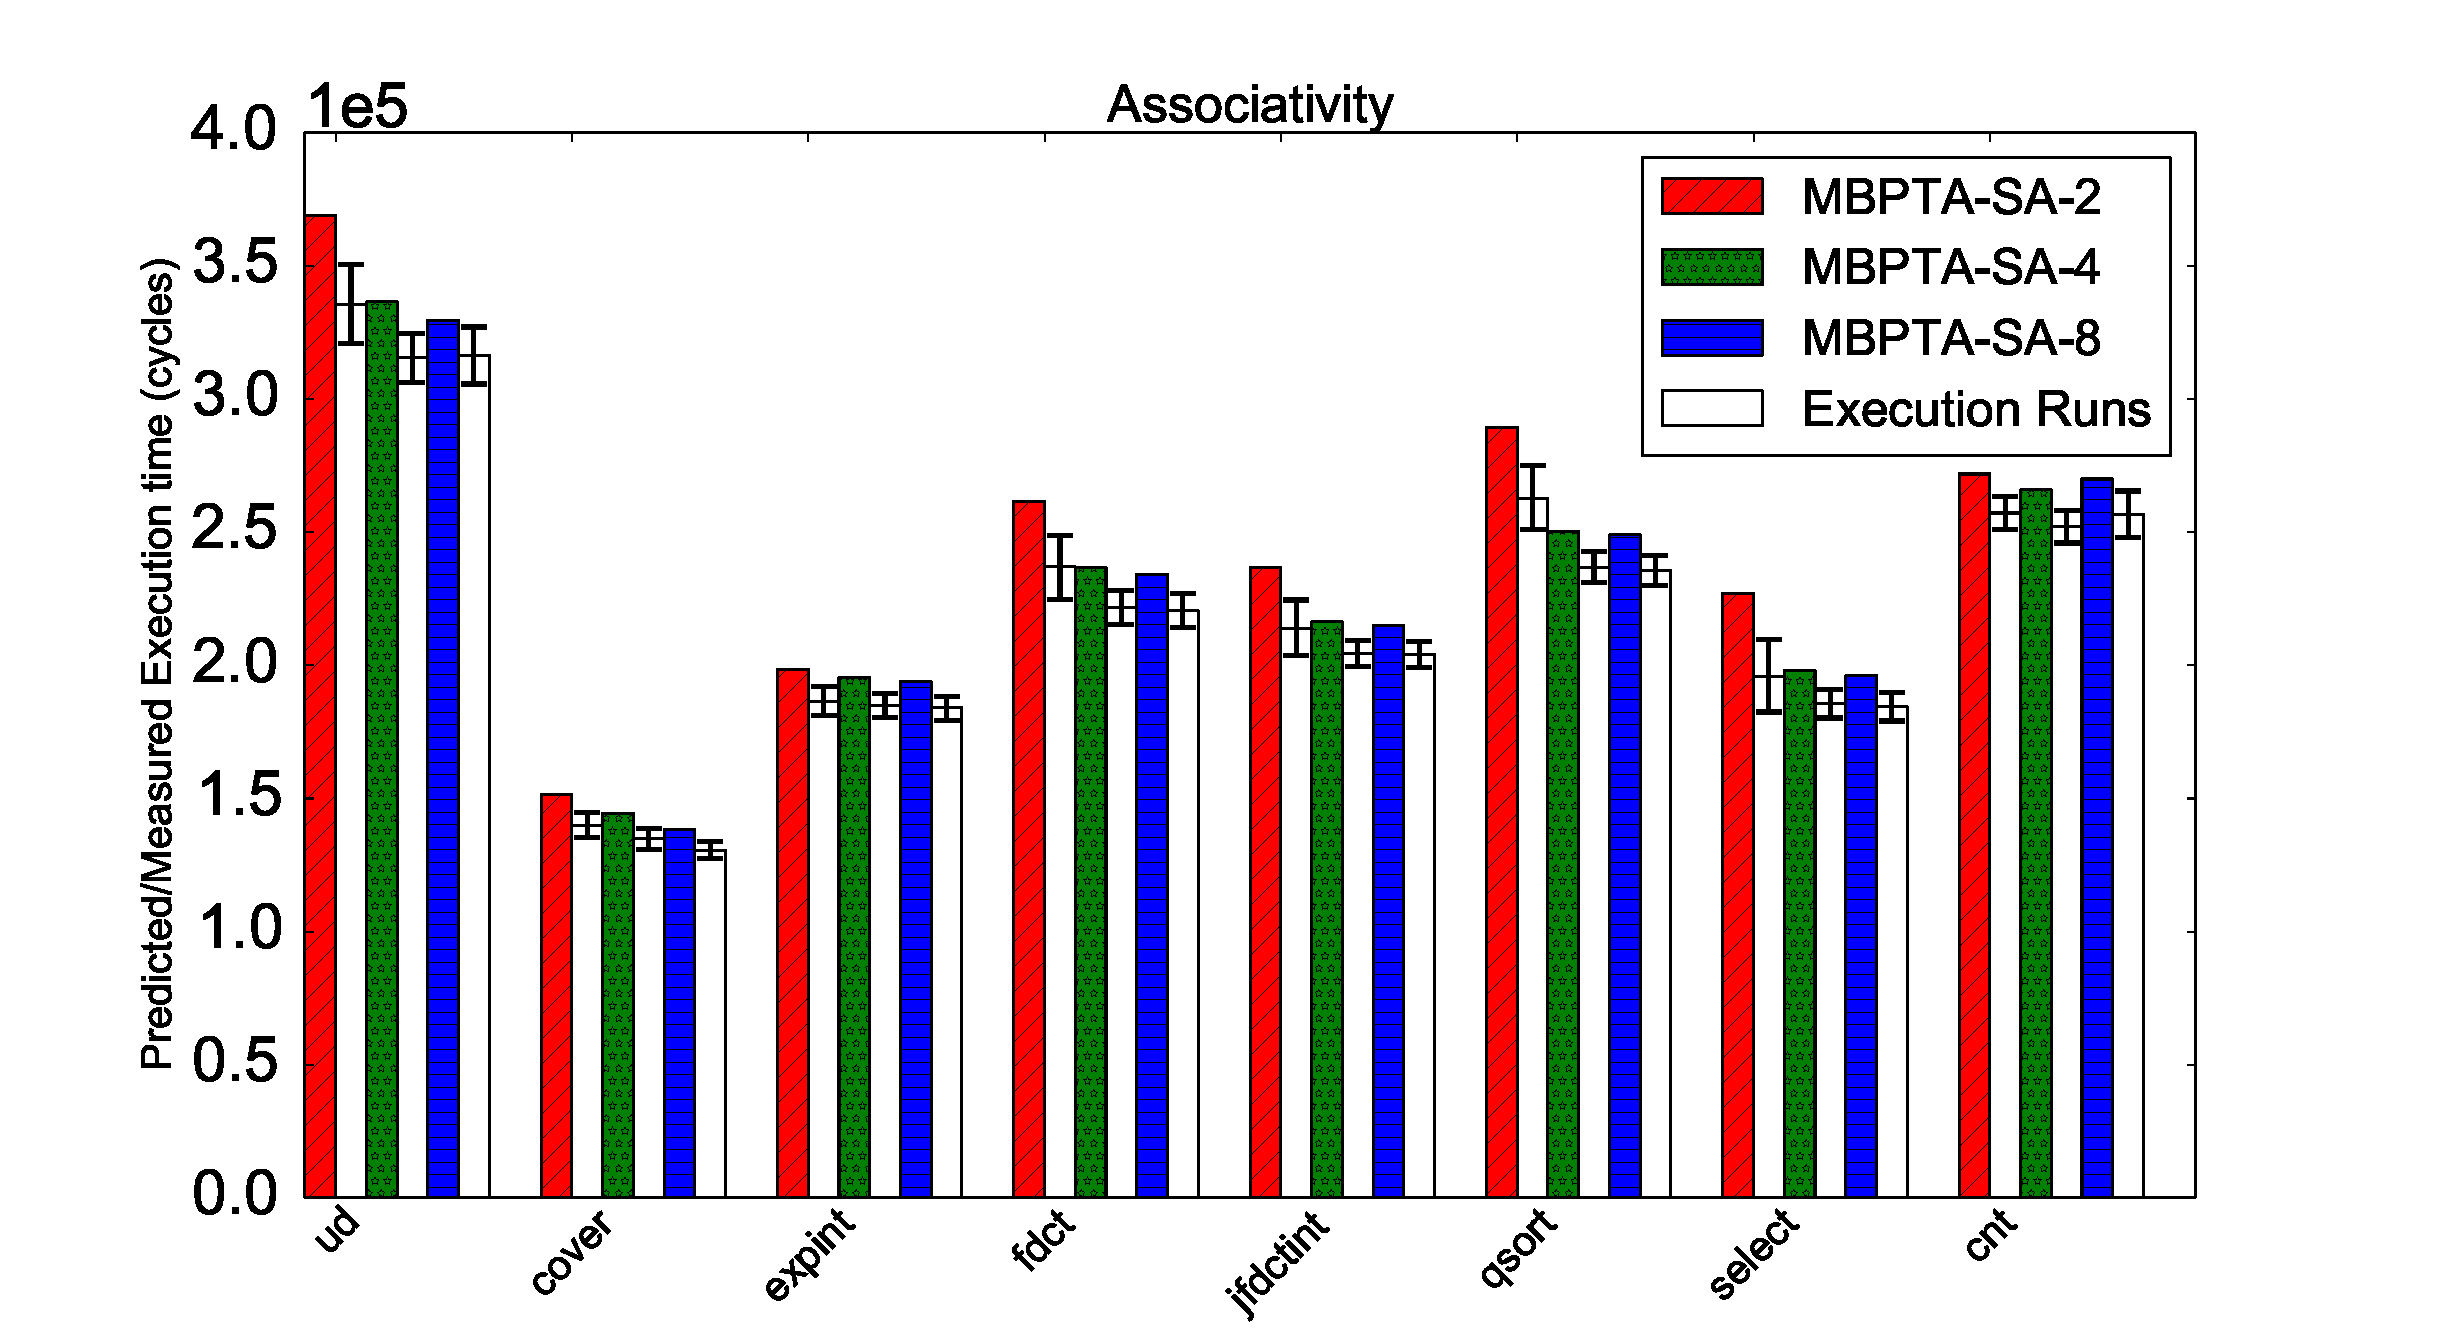
\includegraphics[scale=0.4]{figures/mbpta.pdf}
%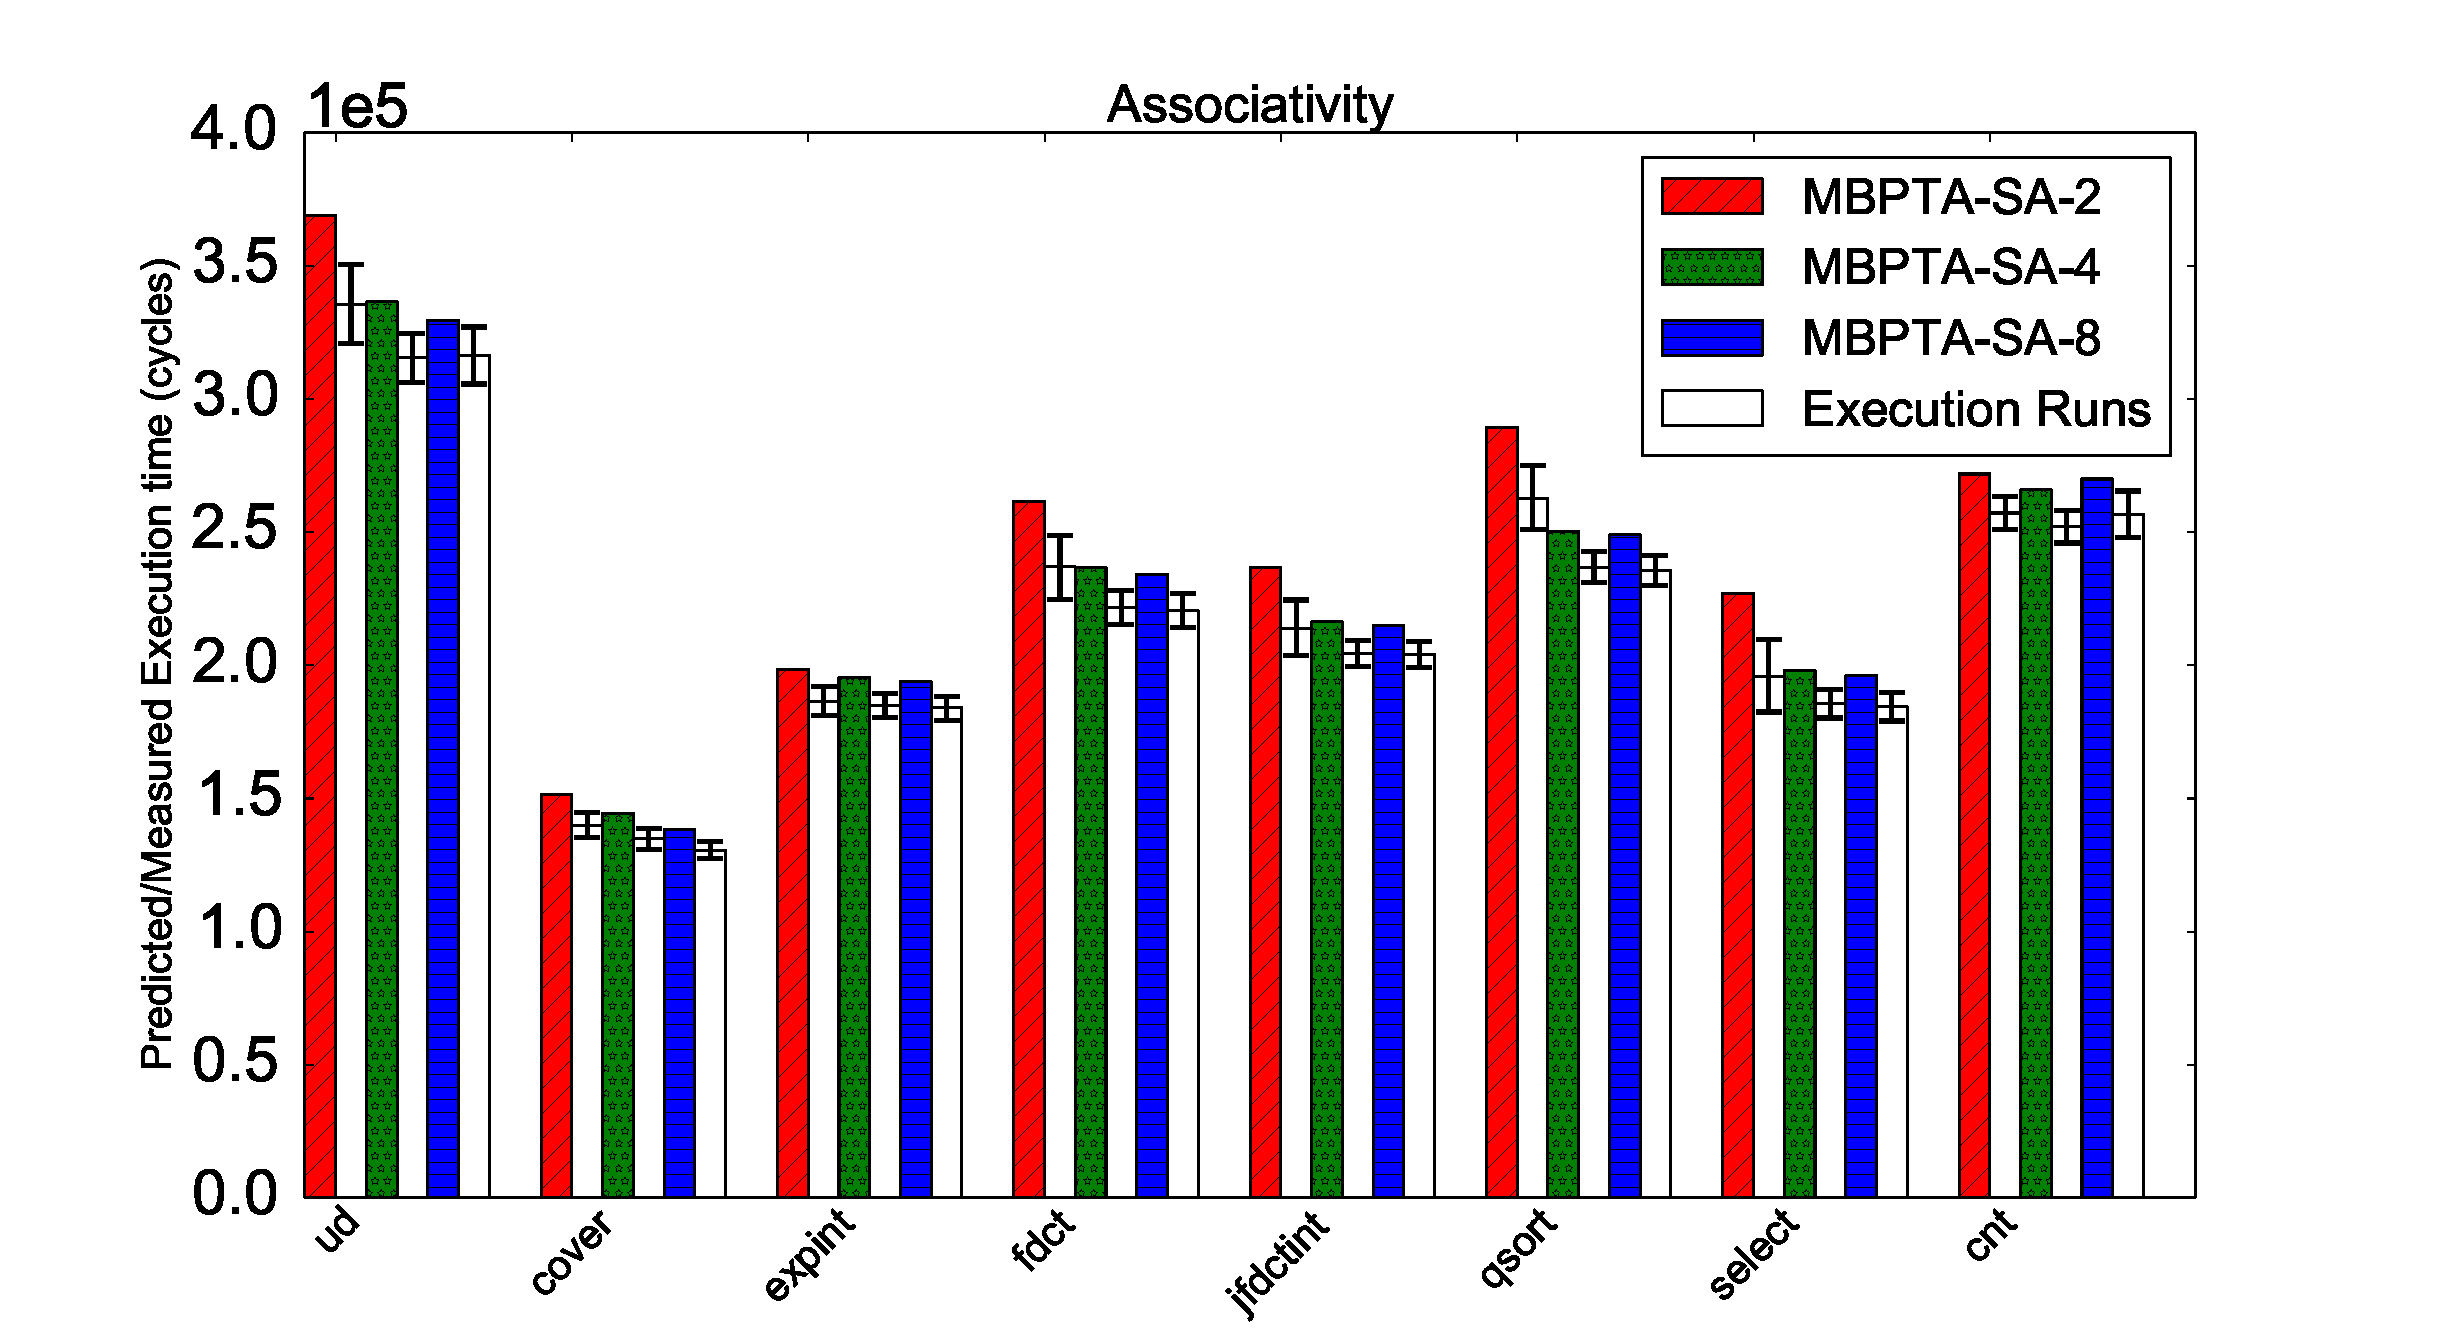
\includegraphics[height=0.4\textheight]{figures/mbpta.pdf}
\caption{Impact on Time-Prediction by varying Associativity-MBPTA.}
\label{fig:MBPTA}
\end{figure}


\subsection{{Prediction Analysis under Associativity}}
The impact and behavior of the time-prediction associated with MBPTA and SPTA under varying associativity is discussed in this section. We also study how cache associativity can counter pessimism. 
Figure~\ref{fig:MBPTA} shows how pessimism varies by changing the cache associativity by applying MBPTA technique. We used three set-associative(SA) cache structures. The cache configuration we used are: SA-2, SA-4, and SA-8 with 2 kB size and 32 bytes line size. We conclude with the following observations (O) under this cache configuration.

%\hspace{-2em}
\textit{\textbf{MBPTA:}}\\
\textit{O-1.1:} The associativity helps to minimize the pessimism because with higher associativity the cache hit ratio improves. The execution-time is also decreased at higher associativity. The higher the associativity, the lower is the  execution-time. Increasing the associativity also improves the prediction estimation because at higher associativity the execution-time distribution getting smooth provide tighter estimates. \\
\textit{O-1.2:} The predicted time (pWCET) is getting closer to the maximum execution-time of a C-code running on a processor by varying the associativity. The higher the associativity, the smaller is the overestimation. For example, for the cache with the associativity-2 (SA-2), the time-prediction is varied between 5.09\% to 3.11\%. This pessimism is decreased from 4.26\% to 1.33\% as shown in Figure~\ref{fig:MBPTA} and summarizes in Table~\ref{percentage difference}. 

\begin{figure}[tb!]
\centering
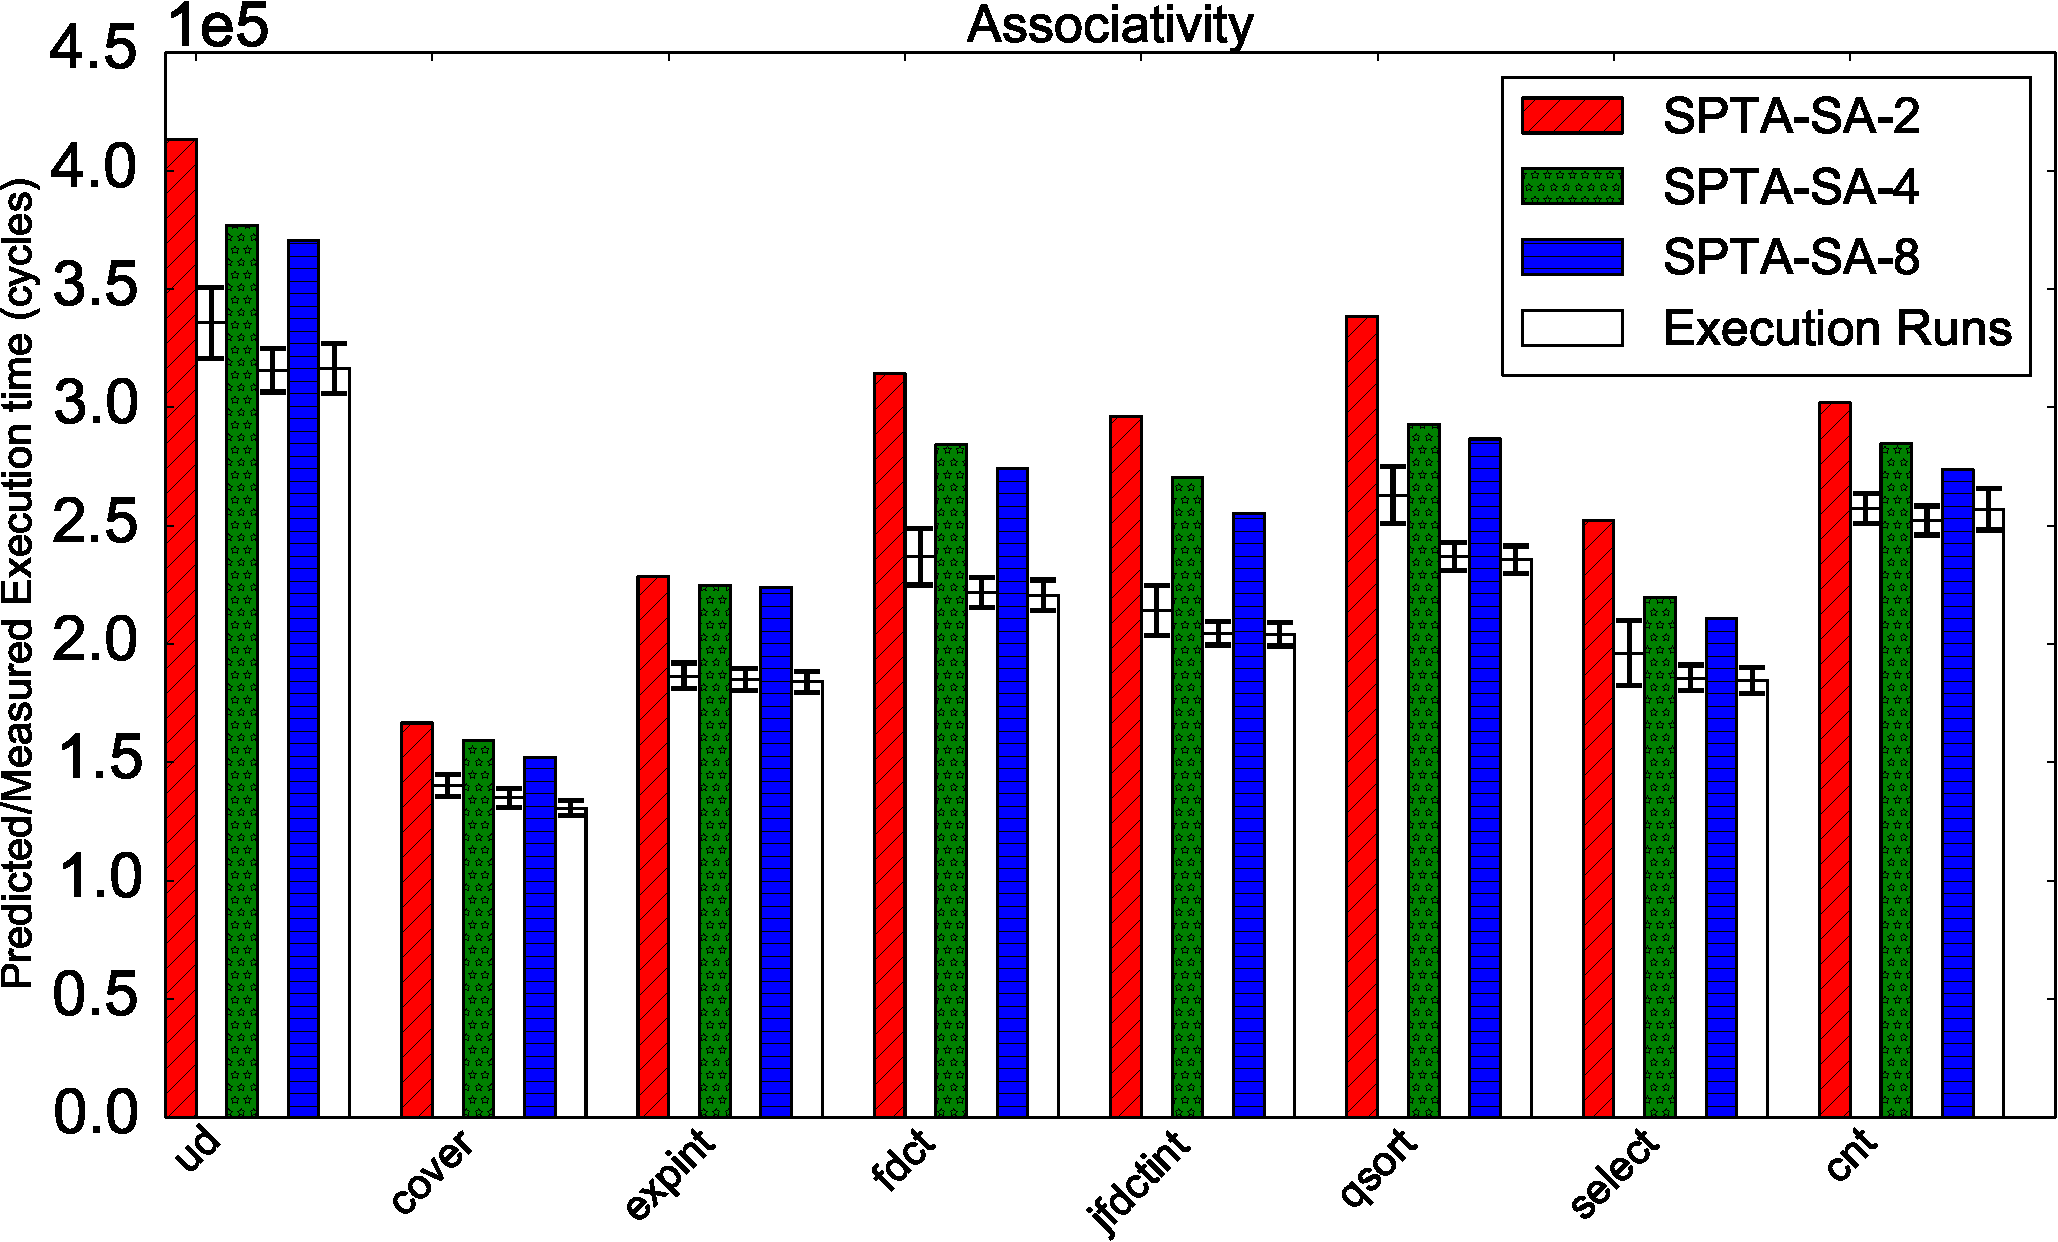
\includegraphics[scale=0.4]{figures/spta.pdf}
\caption{Impact on Time-Prediction by varying Associativity-SPTA.}
\label{fig:SPTA}
\end{figure}

%\hspace{-2em}
\textit{\textbf{SPTA:}}\\
\textit{O-1.3:} The SPTA technique is applied on the address traces of the code. The first observation is about performance: the SPTA performance is not as predictable as  we observed for  MBPTA. The pessimism is always higher for  SPTA as compared with  MBPTA as shown in Table~\ref{percentage difference}.\\
\textit{O-1.4:} The computed pWCETs does not depend on the associativity. Because of the overestimations added by the equation described in section~\ref{spta}, the pessimism does not decrease at higher cache associativity analysed through SPTA. This is due to the fact that the randomized cache needs to ensure the number of misses to ensure independence tests.\\
\textit{O-1.5:} However, we have observed that the pessimism is improved within  SPTA at higher associativity. Particularly, for the \textit{jfdctint, cnt} the pessimism is decreased by 7.76\% and 10.46\% respectively. But pessimism is still higher than we found for the MBPTA.\\
\textit{O-1.6:} The average difference between the predicted time and the maximum execution-time for the SPTA is 3.07\% and 1.77\% for the MBPTA.



\subsection{Prediction Analysis under Cache Size}
We study the effects of the cache size on time-prediction. The level of pessimism achieved varying the cache size is discussed in this section. We performed our test on three different sizes (2 kB, 4 kB, and 8 kB) with 2-way associative cache (SA-2), and the line size is 32-bytes. 

\begin{figure}[tb!]
\centering
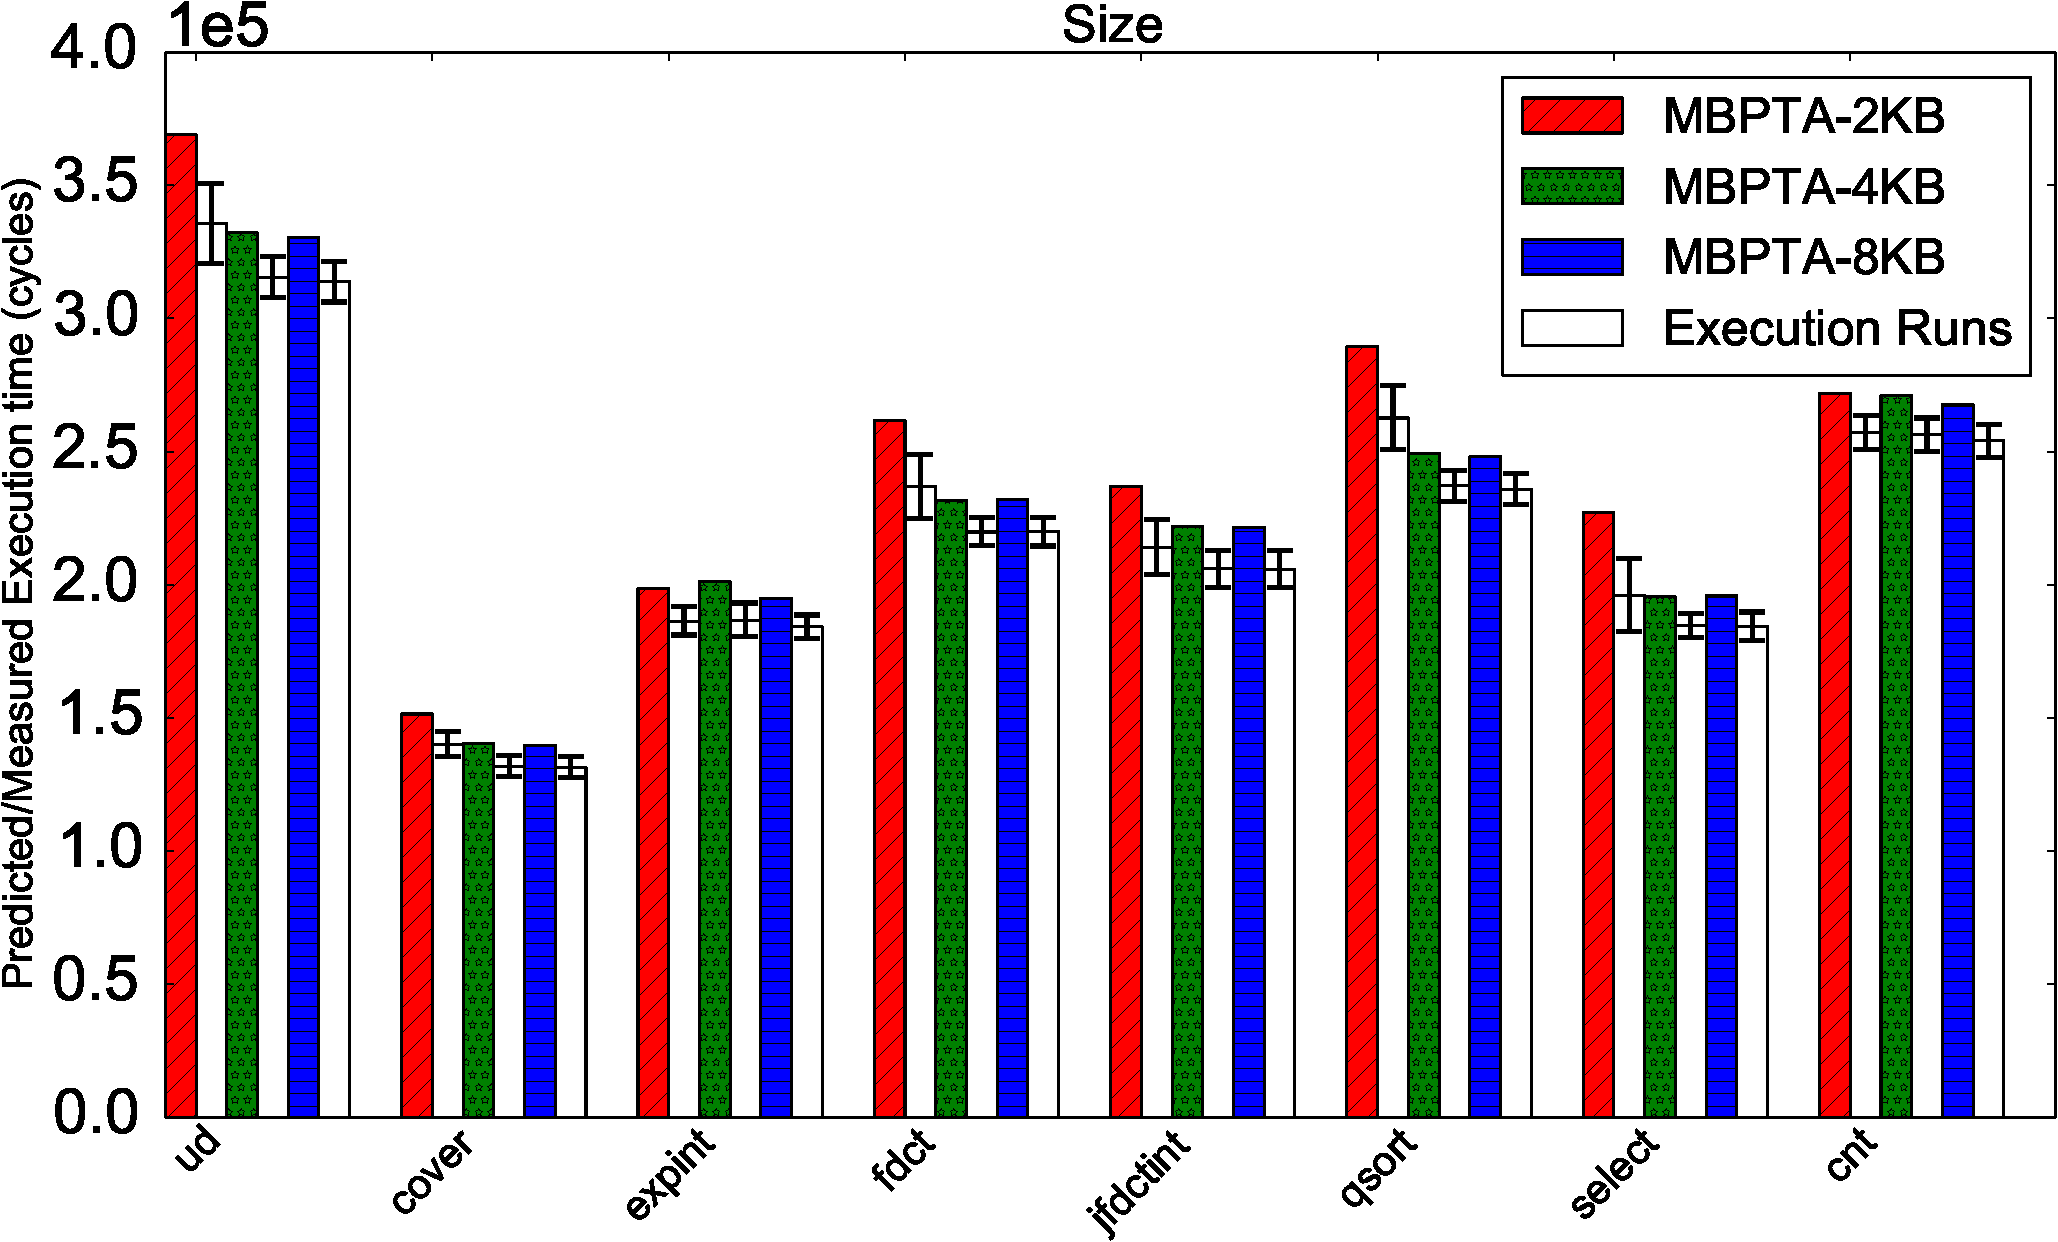
\includegraphics[scale=0.4]{figures/cachesize-mbpta.pdf}
\caption{Impact on Time-Prediction by varying Cache Size-MBPTA.}
\label{Cachesize-MBPTA}
\end{figure}

%\hspace{-2em}
\textit{\textbf{MBPTA:}} \\
The impact of changing the cache size on the time-prediction by employing MBPTA is being studied. Figure~\ref{Cachesize-MBPTA} shows how much pessimism is varied by varying the cache size. We conclude with the following observations under this cache configuration.
\\
\textit{O-2.1:} The prediction difference between the predicted time  and the maximum execution-time is decreased by increasing the cache size. The level of pessimism is decreased from 5.01\% to 0.43\% by increasing the size from 2-kB to 8-kB as summarized in Table~\ref{improvement factor}. Increasing in the cache size helps to fit the binary code size into the cache and this ultimately improves the cache hit ratio.
\\
\textit{O-2.2:} Increasing the cache size helps to decrease the pWCET  estimate. It results in a less pessimistic prediction time. Figure~\ref{Cachesize-MBPTA} shows the effects on the time-prediction under different cache sizes.

%\hspace{-2em}
\textit{\textbf{SPTA:}}\\
\textit{O-2.3:} The behavior obtained by varying the cache size is almost the same the one observed when varying the \textit{associativity}. The pessimistic value is quite higher, that is in between 1.25\% and 3.53\% as shown in the Table~\ref{improvement factor}.
\\
\textit{O-2.4:} The average pessimistic difference between the predicted time and the actual execution-time from 2-kB to 8-kB is 2.38\%. Whereas, for MBPTA, this difference factor is reduced to 1.93\%. SPTA pessimistic nature does not help to minimize the level of pessimism as much MBPTA does.

\begin{figure}[tb!]
\centering
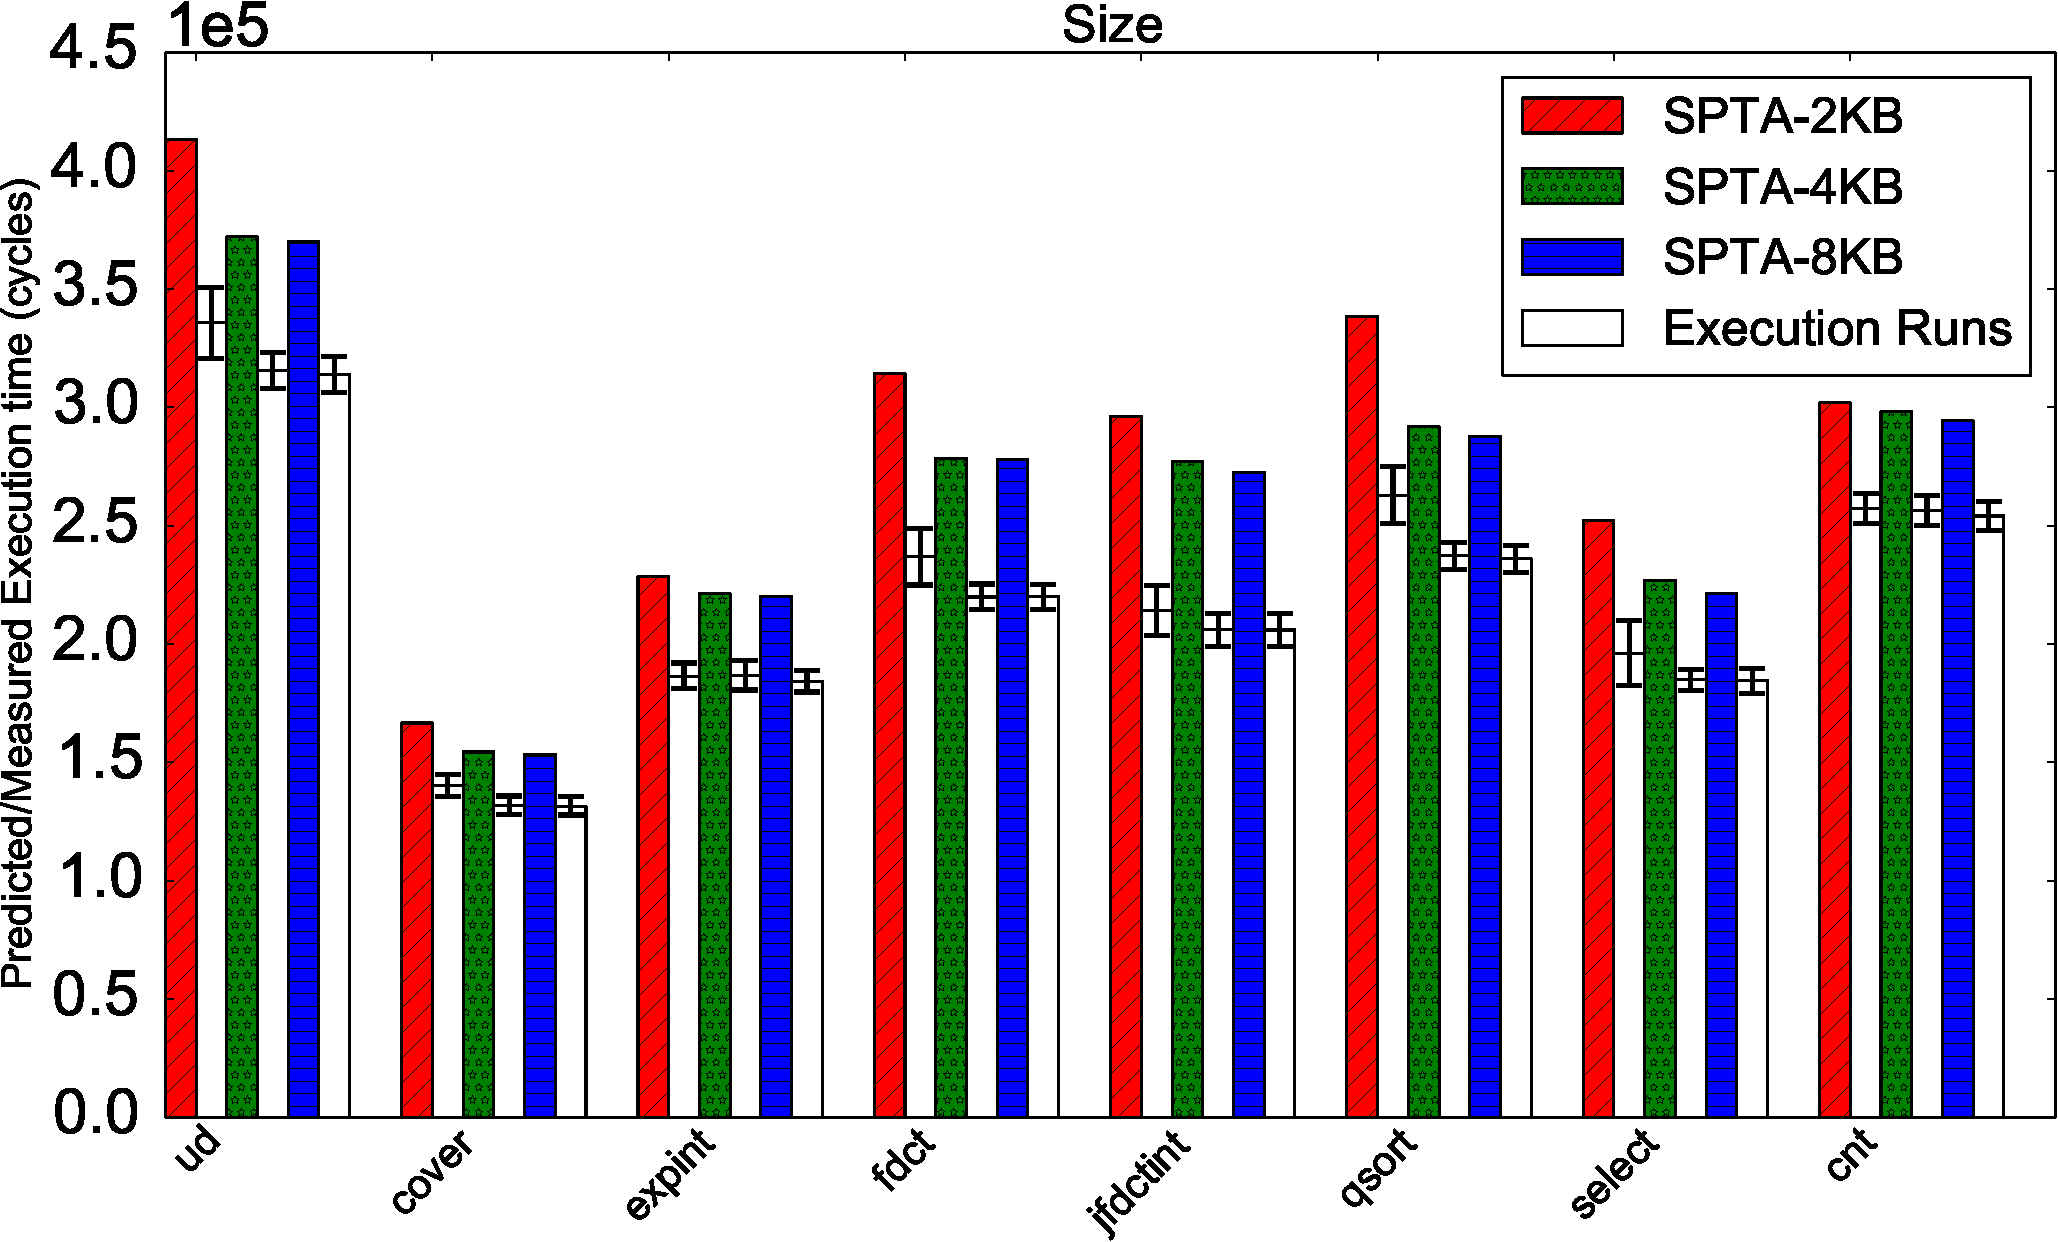
\includegraphics[scale=0.4]{figures/cachesize-spta.pdf}
\caption{Impact on Time-Prediction by varying Cache Size-SPTA.}
\label{Cachesize-SPTA}
\end{figure}

\subsection{{Prediction Analysis under Line Size}}

The impact of the line size on the prediction is shown in Figure~\ref{cacheline-mbpta} when applying MBPTA and Figure~\ref{cacheline-spta} when applying SPTA. We have used two cachelines, i.e. 16-bytes line size and 32-bytes line size with the 4-way associativity, and the capacity is 4-kB. Data and instruction caches are used with the same parameters. 
\\
%\hspace{-2em}
\textit{\textbf{MBPTA}:}\\
\textit{O-3.1:} We have observed that an increase in the line size decreases the pWCET estimate. Because larger cache lines minimize the number of loads from the memory that helps to reduce pessimism. As we observe from Figure~\ref{cacheline-mbpta}, the average reduction in predicted time is 1.87\%.

\begin{figure}[tb!]
\centering
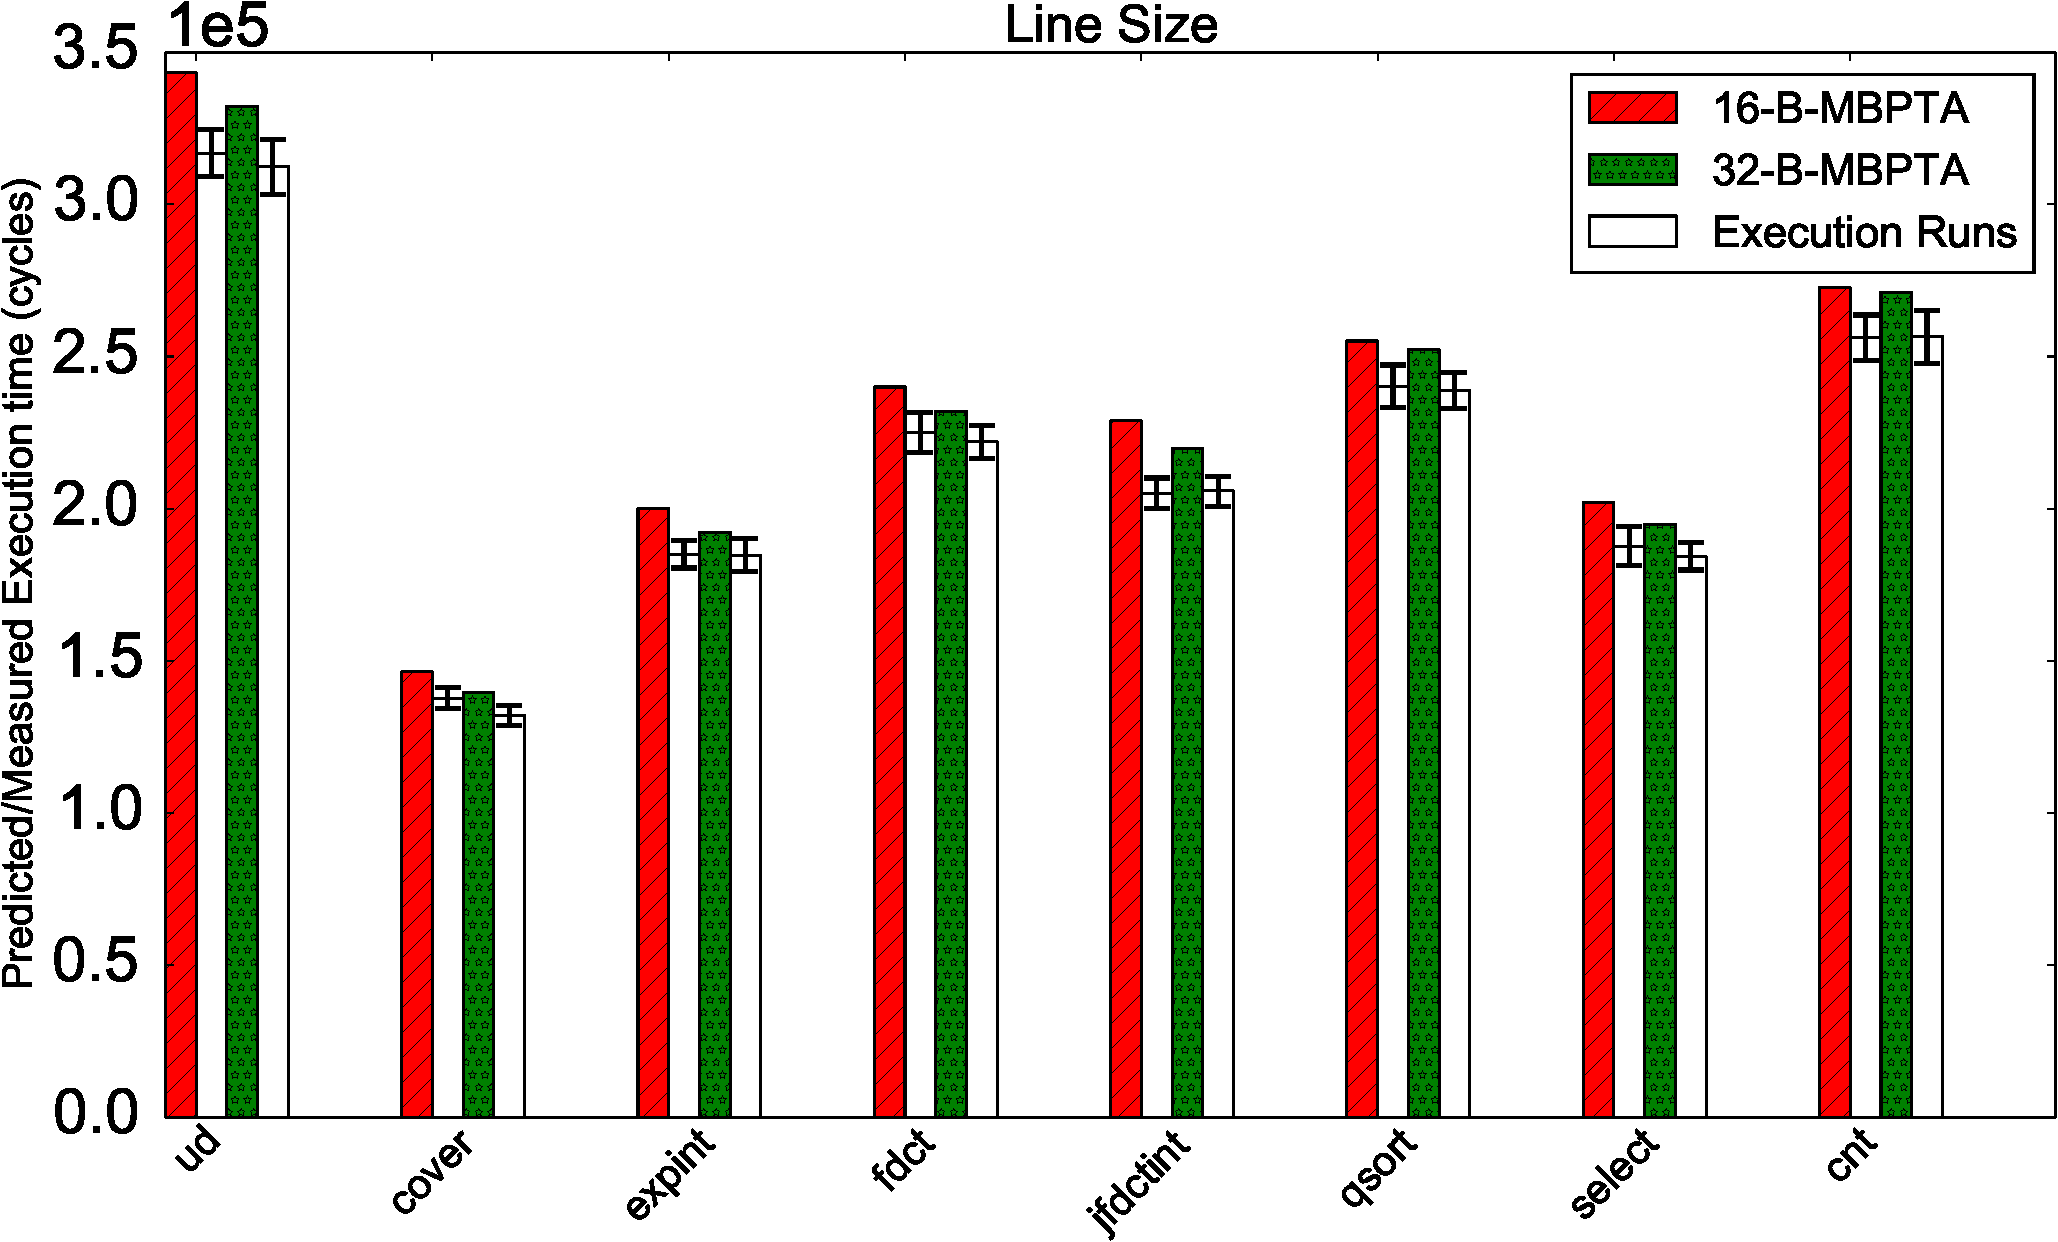
\includegraphics[scale=0.4]{figures/cacheline-mbpta.pdf}
\caption{Impact on Time-Prediction by varying
Cacheline-MBPTA.}
\label{cacheline-mbpta}
\end{figure}




%\hspace{-2em}
\textit{\textbf{SPTA:}}\\
\textit{O-3.2:} We observed the same behavior by varying the line size with SPTA as with MBPTA. The improvement factor is shown in Table~\ref{improvement factor}. The difference between the predicted time and the maximum execution-time for SPTA by varying the line size is remarkably improved compared to varying the associativity and sizes. This is due to the fact that by increasing the line-size helps to minimize the number of loads from the memory as a result improve execution-time and prediction. For example, consider the test case~\textit{Ud} with associativity-4 (SA-4), the level of pessimism goes from 16.39\% to 6.14\% considering the same configuration by varying only the line size. 




\begin{figure}[tb!]
\centering
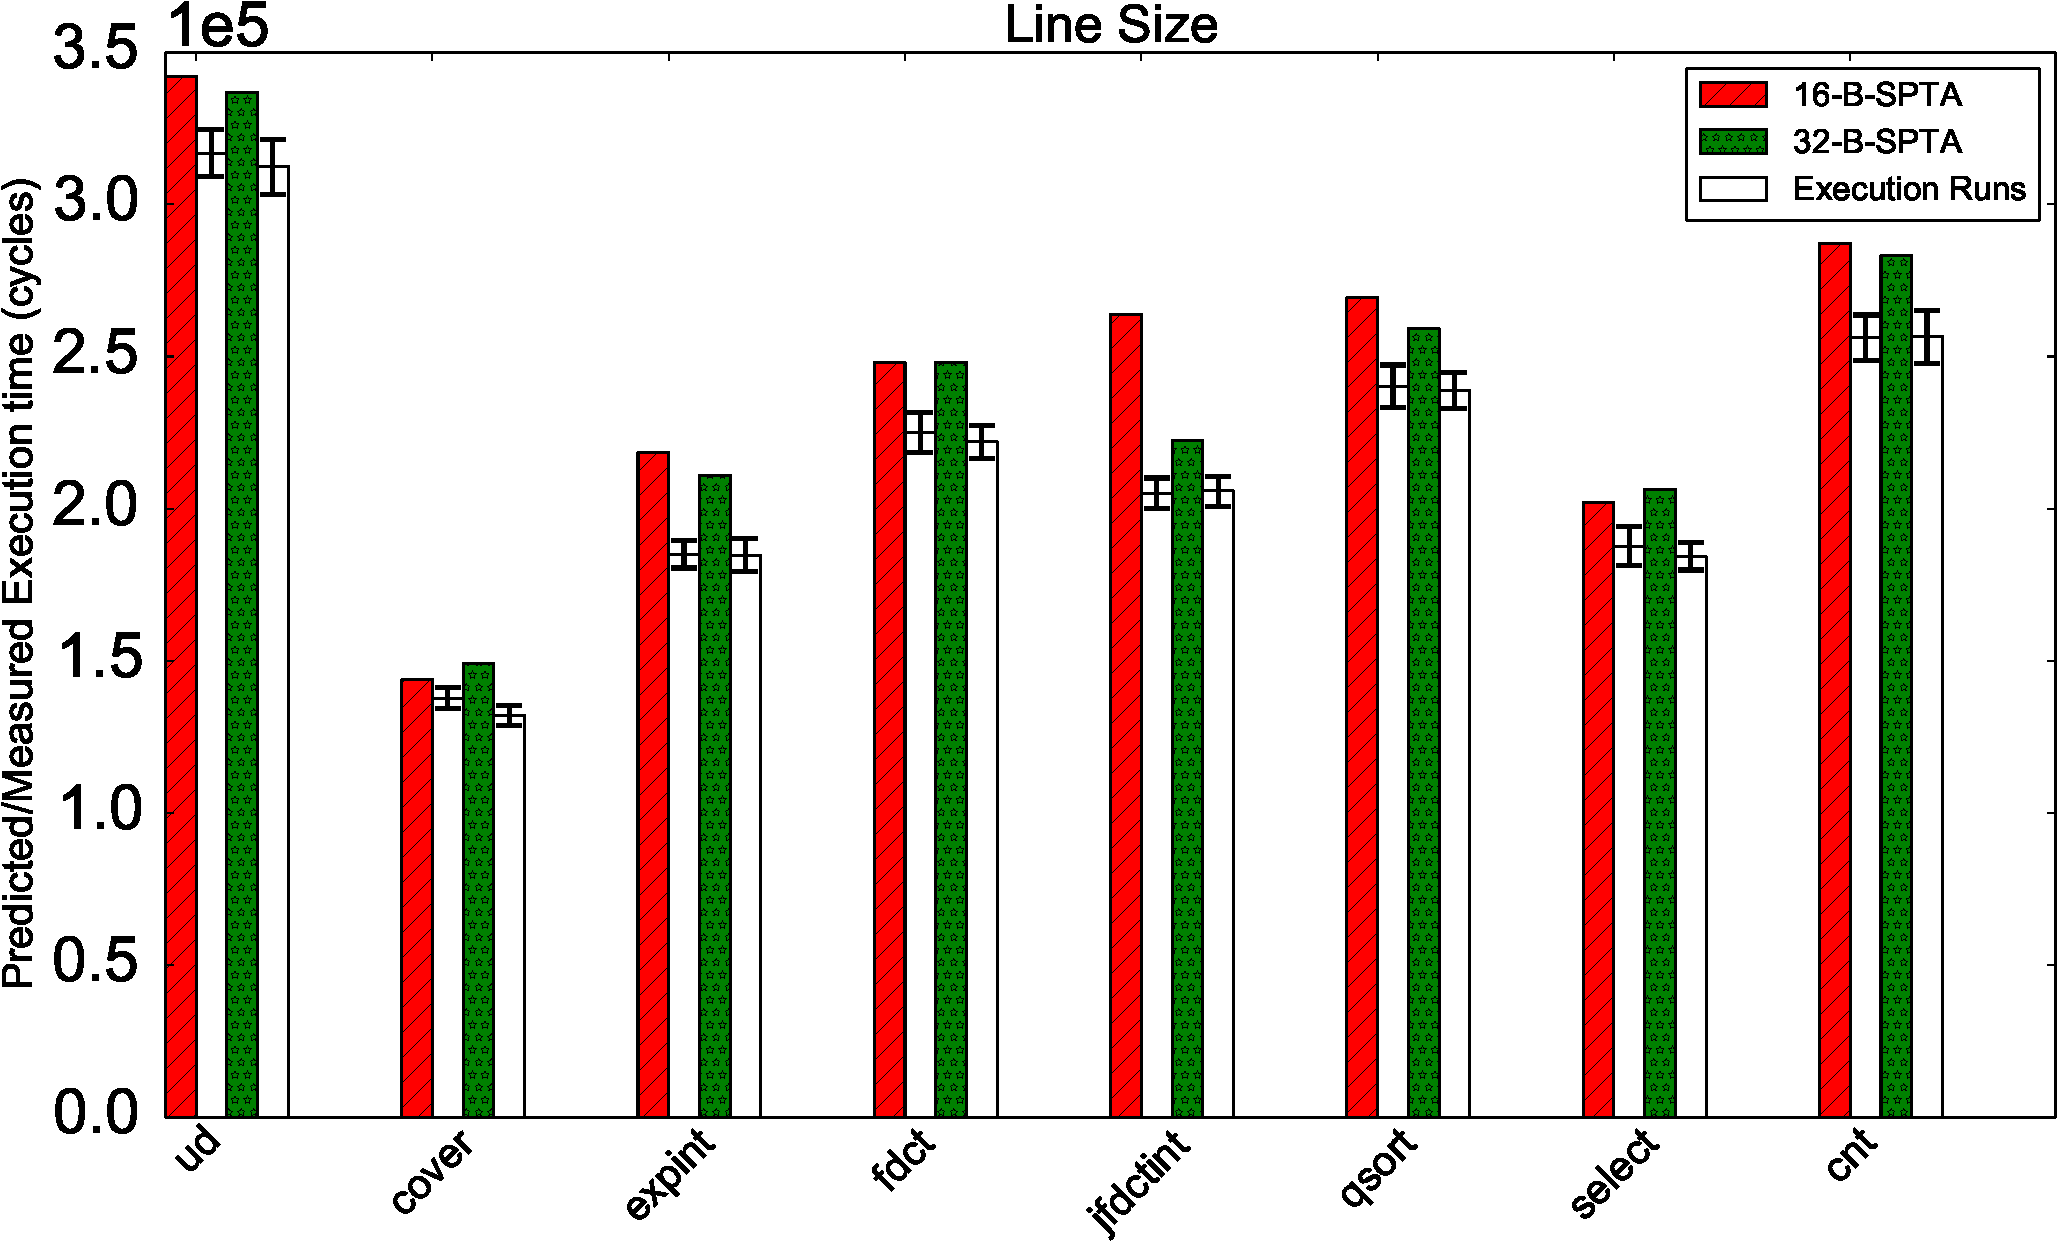
\includegraphics[scale=0.4]{figures/cacheline-spta.pdf}
\caption{Impact on Time-Prediction by varying
Cacheline-MBPTA.}
\label{cacheline-spta}
\end{figure}


\begin{table}[tb!]
\centering

\caption{Level of Pessimism Introduced by varying Cache Parameters.}
%\vspace{-0.7cm}
%\hspace*{-2.3em}
\label{percentage difference}
\scalebox{0.8}{
\centering
\begin{tabular}{lcccccccccccccc}
\toprule
Benchmark & \multicolumn{12}{c}{Level of Pessimism(\%)}   \\
\cmidrule(lr){2-3} \cmidrule(lr){4-5} \cmidrule(lr){6-7} \cmidrule(lr){8-9}\cmidrule(lr){10-11}\cmidrule(lr){12-13}\cmidrule(lr){14-15}


  
  & Associativity      && Associativity && Size &&Size &&Line size && Line size && \\
& \multicolumn{1}{l}{SA-2 to SA-8} &&{SA-2 to SA-8} &&SA 2-8 kB &&SA 2-8 kB && SA 16-32 B && SA 16-32 B && \\ 
& \multicolumn {1}{l}{\hspace{0.5cm}{MBPTA}} &&SPTA &&MBPTA &&SPTA&&MBPTA &&SPTA && \\
  \midrule




 
ud       &   \multicolumn{2}{c}{4.26} & \multicolumn{2}{c}{3.96} & 
\multicolumn{2}{c}{2.27} & \multicolumn{2}{c}{2.26} 
& \multicolumn{2}{c}{2.43} & \multicolumn{2}{c}{2.37}


  \\ 
cover    &   \multicolumn{2}{c}{1.24} & \multicolumn{2}{c}{1.23} &
\multicolumn{2}{c}{1.13} & \multicolumn{2}{c}{1.41} 
& \multicolumn{2}{c}{0.45}
& \multicolumn{2}{c}{0.52}
\\

expint &   \multicolumn{2}{c}{\color{red}{0.95}}    & \multicolumn{2}{c}{\color{red}{0.43}} &
\multicolumn{2}{c}{0.43}&\multicolumn{2}{c}{2.21}
& \multicolumn{2}{c}{4.12}
& \multicolumn{2}{c}{3.27}
\\ 

fdct     &   \multicolumn{2}{c}{1.70}& \multicolumn{2}{c}{4.18}
& \multicolumn{2}{c}{1.99} & \multicolumn{2}{c}{2.06} 
& \multicolumn{2}{c}{1.58}
& \multicolumn{2}{c}{1.81}
\\ 

jfdctint &   \multicolumn{2}{c}{2.74} & \multicolumn{2}{c}{7.76}&
\multicolumn{2}{c}{\color{red}{1.57}}&\multicolumn{2}{c}{\color{red}{3.13}}
& \multicolumn{2}{c}{4.49}
& \multicolumn{2}{c}{3.23}
\\ 

qsort-exam & \multicolumn{2}{c}{2.21} & \multicolumn{2}{c}{3.82} &
\multicolumn{2}{c}{2.70}&\multicolumn{2}{c}{3.53}
& \multicolumn{2}{c}{0.15}
& \multicolumn{2}{c}{0.70}
 \\ 

select     & \multicolumn{2}{c}{4.80} & \multicolumn{2}{c}{7.93} &
\multicolumn{2}{c}{5.01}&\multicolumn{2}{c}{3.21} 
& \multicolumn{2}{c}{\color{red}{0.88}}
& \multicolumn{2}{c}{\color{red}{0.62}}

\\


cnt        & \multicolumn{2}{c}{1.33} & \multicolumn{2}{c}{10.46} &
\multicolumn{2}{c}{0.35} & \multicolumn{2}{c}{1.25} 
& \multicolumn{2}{c}{1.11}
& \multicolumn{2}{c}{0.82}
\\
\bottomrule
\end{tabular}
}
\end{table}




\begin{figure}[tb!]
\centering
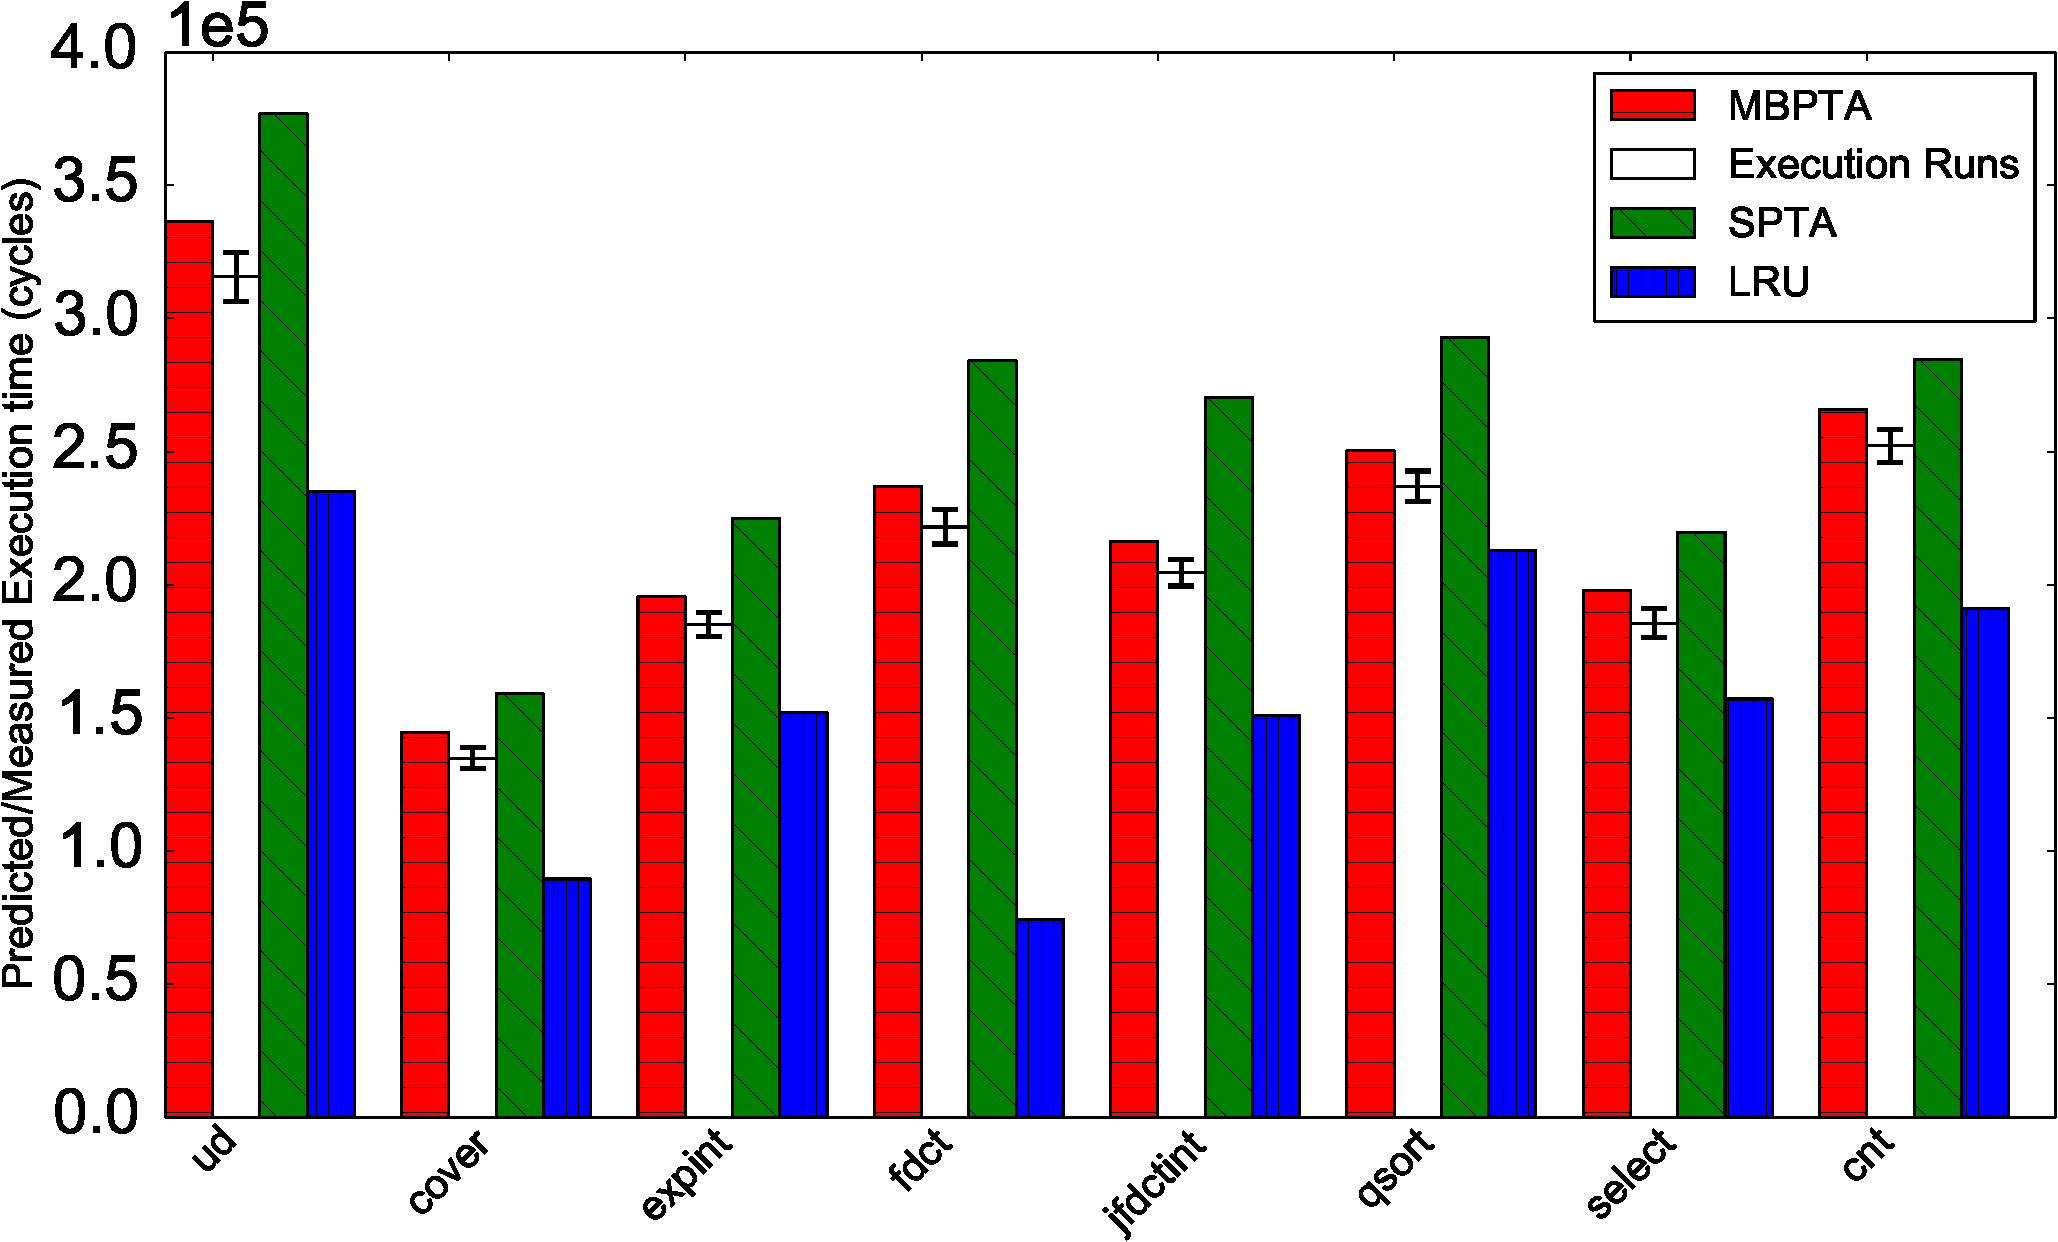
\includegraphics[scale=0.4]{figures/comparison.pdf}
\caption{Comparison between Time-Prediction via Timing Techniques and Maximum Execution-Time.}
\label{comparison}
\end{figure}

\begin{table}[tb!]
\caption{Deterministic/Probabilistic WCETs and respective Execution Bounds.}
\centering
\label{det2}
%\hspace{2.8cm} 
\scalebox{0.75}{
%
\begin{tabular}{lccccccccccc}
\toprule
Benchmark & \multicolumn{9}{c}{Execution-Time (clock cycles)} & &  \\
\cmidrule(lr){2-2} \cmidrule(lr){4-4} \cmidrule(lr){6-6} \cmidrule(lr){8-8}
 \cmidrule(lr){10-10}

& Deterministic  & & Prediction  & & Probabilistic & & Prediction  & & Prediction\\
 &  \multicolumn{1}{l}{\hspace{0.5cm}{Cache (WCET)}} & & bound & & Cache (WCET) & & bound (MBPTA) & & bound (SPTA)\\
  
 

  \midrule

ud       &   \multicolumn{2}{c}{235050} & \multicolumn{2}{c}{386920}    & \multicolumn{2}{c}{324950} & \multicolumn{2}{c}{376500} & \multicolumn{2}{c}{376880} \\

cover       &   \multicolumn{2}{c}{107894} & \multicolumn{2}{c}{159792}    & \multicolumn{2}{c}{138798} & \multicolumn{2}{c}{154526} & \multicolumn{2}{c}{158978} \\

expint       &   \multicolumn{2}{c}{152020} & \multicolumn{2}{c}{234689}    & \multicolumn{2}{c}{189380} & \multicolumn{2}{c}{225458} & \multicolumn{2}{c}{224776} \\

fdct       &   \multicolumn{2}{c}{217066} & \multicolumn{2}{c}{291194}    & \multicolumn{2}{c}{218092} & \multicolumn{2}{c}{234587} & \multicolumn{2}{c}{284119} \\

jfdctint      &   \multicolumn{2}{c}{150850} & \multicolumn{2}{c}{270891}    & \multicolumn{2}{c}{209487} & \multicolumn{2}{c}{266357} & \multicolumn{2}{c}{270446} \\

qsort       &   \multicolumn{2}{c}{212880} & \multicolumn{2}{c}{294480}    & \multicolumn{2}{c}{242609} & \multicolumn{2}{c}{280291} & \multicolumn{2}{c}{292840} \\

select       &   \multicolumn{2}{c}{157060} & \multicolumn{2}{c}{224975}    & \multicolumn{2}{c}{190812} & \multicolumn{2}{c}{217977} & \multicolumn{2}{c}{219754} \\

cnt       &   \multicolumn{2}{c}{190980} & \multicolumn{2}{c}{289654}    & \multicolumn{2}{c}{258480} & \multicolumn{2}{c}{285921} & \multicolumn{2}{c}{286535} \\



\bottomrule
\end{tabular}
}
\end{table}


\begin{table}[h]
\caption{Pessimism between Predicted pWCETs at $10^{-3}$ Exceedance Probability versus Deterministic Cache.}

\label{improvement factor}
\centering
\scalebox{0.8}{

\begin{tabular}{lccccccccc}
\toprule
 & \multicolumn{9}{c}{Pessimism Difference(\%)}   \\
\cmidrule(lr){2-2} \cmidrule(lr){3-3} \cmidrule(lr){4-4} \cmidrule(lr){5-5} \cmidrule(lr){6-6} \cmidrule(lr){7-7} \cmidrule(lr){8-8} \cmidrule(lr){9-9}


  
 & ud     & cover   & expint  & fdct &  jfdctint &  qsort &select &cnt  \\


  \midrule

Deterministic cache       &   \multicolumn{1}{c}{49.67}  
 
 & \multicolumn{1}{c}{39.55} &

 \multicolumn{1}{c}{43.80} 
  &    \multicolumn{1}{c}{29.13} & \multicolumn{1}{c}{57.55} & \multicolumn{1}{c}{33.09} & \multicolumn{1}{c}{36.22} &\multicolumn{1}{c}{41.38} & \\
 
Probabilistic cache (MBPTA)       &   \multicolumn{1}{c}{14.70} &

 \multicolumn{1}{c}{10.72}  &\multicolumn{1}{c}{17.39}
  &   \multicolumn{1}{c}{7.07} &   \multicolumn{1}{c}{23.90}& \multicolumn{1}{c}{14.41} & \multicolumn{1}{c}{13.29} & \multicolumn{1}{c}{10.08}   \\
  
  Probabilistic cache (SPTA)       &   \multicolumn{1}{c}{14.80} &

 \multicolumn{1}{c}{13.55}  &\multicolumn{1}{c}{17.09}
  &   \multicolumn{1}{c}{26.29} &   \multicolumn{1}{c}{25.40}& \multicolumn{1}{c}{18.70} & \multicolumn{1}{c}{14.10} &\multicolumn{1}{c}{10.30}  \\
  
  
 
\bottomrule
\end{tabular}
}
\end{table}





%\hspace{-2em}
\textit{\textbf{Summary:}} Figure~\ref{comparison} shows a comparison between the deterministic cache enabled with modulo placement and LRU replacement for  probabilistic cache used MBPTA and SPTA it also shows the comparison with the maximum measured execution-time. The result presented in Figure~\ref{comparison} is derived from the cache configuration \textit{SA-4, size-2 kB, and line-size-32 byte}. We observed that the level of pessimism associated with a deterministic cache (analyzed with DTA) is higher than MBPTA and SPTA (probabilistic cache) as compared to the maximum execution-time.  Performance in terms of prediction is lower for the deterministic cache. We observed that the prediction obtained with MBPTA and SPTA is closer to the actual execution-time. The results obtained for the deterministic cache are underestimated and they are quite far from the real execution-time as shown in Figure~\ref{comparison} and summarized in Table~\ref{det2}. This also proves the point we made in section~\ref{intro}, that probabilistic techniques performed well with randomized architecture. This result also shows a comprehensive qualitative analysis that each technique is particularly suitable for specific set of software and hardware. SPTA shows more pessimism than MBPTA because SPTA is more sensitive to the knowledge of referenced addresses. It means EVT based MBPTA provides tightest pWCET estimations compared to SPTA. 


\begin{figure}[tb!]

% \centering
 % \captionsetup{justification=centering}  
  
   
   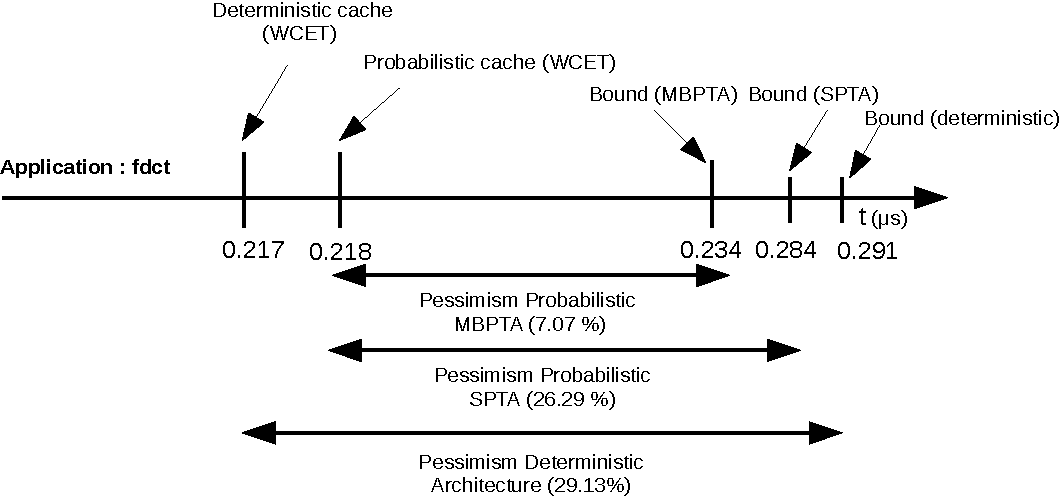
\includegraphics[scale=0.8]{figures/tpc-example2.pdf}

\caption{Pessimism between Predicted pWCETs at $10^{-3}$ Exceedance Probability versus Deterministic Cache.} 
\label{application:fdct}
\end{figure}
Similarly, Table~\ref{det2} shows the deterministic and probabilistic WCETs and respective bounds. These results can be summarized in 
Table~\ref{improvement factor} which shows the pessimism difference between the MBPTA, SPTA, and deterministic cache.  We used application \textbf{fdct} to elaborate the pessimism obtained by MBPTA is minimum as compared it with the SPTA and deterministic architecture shown in Figure~\ref{application:fdct}.  In summary, our tests show that the randomized cache can be used to apply MBPTA and SPTA techniques to find the time-predictions and associated pessimism.
In short, compared to deterministic cache the observed execution-time and associated pessimism is improved
 for probabilistic cache. The difference between the deterministic cache execution-time and its associated prediction bounds is more pessimistic than the difference between the probabilistic cache execution-time and its associated prediction bounds. 
 


\section{Discussion}

The main ideas of the work presented in this thesis are the design of a probabilistic system and analysis of this system with probabilistic timing analysis techniques to measure the time- prediction in terms of pWCET. 
%We redefine the concept of execution-time profiles to describe the probabilistic timing behaviour of the codes. The motivation of this work following observation: \textit{The static WCET analysis is the complex technique, mainly due to the necessity of building an as-precise-as-possible view of impact of the execution history on the hardware state at each time of the program. The over-approximation of this impact may degrade the accuracy of the WCET estimation. To overcome the modeling of the execution history, the probabilistic approach randomized the timing behaviour of a hardware component, _{•} randomized cache. This results in a smooth distribution of the execution-time probabilities. Then, a WCET probability distribution is computed   using a technique based on EVT named MBPTA and to measure the execution-time probability distribution for individual operations, e.g. memory accesses named SPTA} 

To get promising results and make the system probabilistically analyzable, a randomized cache is used. The randomized cache fulfills the requirements that are necessary for the probabilistic timing techniques, e.g., the \textit{i.i.d} property. Probabilistic timing techniques in both variants---static and measurement-based techniques---are used. The MBPTA used the execution-time of the program. The execution-time is obtained by running the benchmark which comprises of C-code on the randomized hardware. The timing information is given to the MBPTA method and produced a tight pWCET estimation bound. Second, we used an SPTA method which used memory traces to find an upper bound for the WCET.  

The PTA techniques produced probabilistically accurate WCET estimations that helped to find the execution bounds. The  WCET estimation observed under probabilistic methods provided less pessimism when compared to the execution bound found on a deterministic architecture, e.g., a \textit{lru} cache.
    
    
 %How and why I did it
    
In accordance with the literature, to achieve the necessary requirements for the probabilistic techniques~\cite{Cazorla:2013:PPA:2465787.2465796}, a  randomized cache is used under PTA techniques. The randomized cache is used to generate randomization of the timing behavior. Randomized placement and replacement policies is adopted in this work. A parametric hash function is used for the random placement policy, and a random number generator is used for the random replacement policy. Then, the randomized cache is integrated with the processors. We used two processors: MIPS-32 and Leon-3. The M\"alardalen real-time benchmark is used for in our tests. The C-code is compiled with gcc and machine code is fed to the processors. We executed the same C-code/application several thousand times to obtain the execution-time measurements profile. The measurements we got consist of different timing values which correspond to the execution-times of the benchmark. To verify whether these timing values fulfill the requirements for PTA techniques, independence and identical distribution tests are applied on the timing values. After the successful verification of independence and identical distribution, measurement and static probabilistic techniques are used to establish the probabilistic WCET bound.
    
 %Why
 
    
The PTA approach incurred the timing analysis wall. The static timing analysis methods failed to find solutions for the WCET estimation for complex hardware systems. This is because---as the complexity of the system is increased---driving the accurate, detailed knowledge of the hardware model is a cumbersome job. Furthermore, obtaining the detailed knowledge of the timing behavior of the program in the presence of varying hardware condition (e.g., knowledge of all previously executed instructions) is also a  difficult job. Due to these limitations, PTA techniques emerged that are capable of removing the requirements for the detailed knowledge of the hardware and producing tightly bound WCET estimations. The obtained tight WCET estimations had less dependence on the execution history and required less platform knowledge. The lack of platform knowledge had an influence on the WCET estimations and provided execution bounds that are independent of the platform knowledge. We believe that the required knowledge needed to achieve reliable pWCET bounds can be accomplished by using the hardware platform whose execution-time does not depend on the execution history. The results obtained by applying PTA techniques on the randomized hardware are less pessimistic WCET estimations as compared with the deterministic timing analysis approach.
%We used two versions of probabilistic timing analysis. 
     
    
    
 %   What I Found (Answered the Research Questions)
    
%    In order to apply PTA techniques we employed randomized hardware by using the randomized cache.  . 
    
We discovered that the pessimism associated with PTA techniques is closed enough to the actual measurement as compared to the static approach. The primary objective of the PTA techniques is to provide a tight WCET estimation that is safe enough for the software program and to keep the overall system failure rate lower than the derived bound. The measurement-based probabilistic technique provides a pWCET estimation. The estimation achieved under MBPTA technique is end-to-end runs of a program. The pWCET observed under MBPTA is less pessimistic as compared to the static probabilistic method. In fact, MBPTA derived tight bounds are based on the actual observations rather than the convolution operation which are used by SPTA. To give evidence for our argument---that the pWCET estimations observed under the probabilistic techniques had less pessimistic and tightly bound to the actual measurements rather than the deterministic approach---we used a deterministic architecture, i.e. a LRU replacement and modulo placement. The deterministic approach had a better average performance but provides a high level of pessimism that sets the actual bound away from the real measurements. Setting the pWCET bound away from the actual measurements did not help real-time system designers to design a system with better schedulability analysis and best resource consumption. 
 
 
    
    %What was congruent with the literature?
    
The work accomplished so far in real-time systems timing analysis  is mainly based on simulators rather than real hardware. The results and mathematical foundations presented in~\cite{kosmidis2014measurement},~\cite{abella2014comparison},~\cite{Kosmidis:2013:CDP:2485288.2485416} support our findings. We can relate our findings to the work presented in the literature to support our work. As suggested by the work presented in~\cite{quinones2009using}, we found that the pWCET of a program under varying memory layout is suitable to apply PTA techniques. The authors used different memory layouts to get different timing values. The performance degrades with random policies as compared to other deterministic policies but it had an acceptable average case performance. Based on this observation, the authors developed their PTA techniques by using associative caches with random replacement policies~\cite{Kosmidis:2013:CDP:2485288.2485416}. We used the same strategy using randomized cache placement and replacement policies and analyzed the whole system with PTA techniques. We observed  that it coincided with the theory and the general perception about the PTA techniques. The PTA techniques provide tightly bound pessimism associated with pWCET rather than improving the best execution-time. 
    
    
   % What was surprising?
   %   What are the implications for practice?
%    What are the implications for research?
%    What are the limitations to the study
It is arguable that PTA techniques on randomized architectures are not suitable to improve the average case performance. Why should it be used in real-time systems? In real-time systems, the main focus is on the accurate prediction rather than average case performance improvement. Probabilistic techniques allow reducing the overestimation produced by traditional timing analysis approaches. This work is focused on single core architectures to develop a methodology to apply PTA techniques. The probabilistic approach on a multi-core architecture will be a best possible extension of this work. The problem associated with the use of multi-core architecture in real-time systems is task allocation. It is a challenging task to predict how the task will interact with each other in shared hardware resources. We believed that probabilistic techniques will be a promising solution to find pWCET bound for a multi-core architecture. Moreover, by employing an L2 cache, it will be interesting to see that how it influences the time predictability. Finally, an extension of this work could be the creation of a whole hardware architecture randomized with a randomized bus, TLBs, in order to measure the effects that randomization may introduce on the other components for pWCET estimation. 


\section{Conclusion}

The implementation of a time-predictable architecture, analyzed by probabilistic timing analysis (PTA) techniques is presented. As our target domain is a real-time industry, we stressed the importance of the worst-case execution-time (WCET) estimation. We redefined the concept of execution-time profiles to describe the probabilistic timing behaviour of our sources. The motivation of this work is based on the following observation: 

\textit{The static WCET analysis is a complex technique mainly due to the necessity of building an as-precise-as-possible view of the impact of the execution history on the hardware state at each execution of the program. The over-approximation of this impact may degrade the accuracy of the WCET estimation. To overcome the modeling of the execution history, a probabilistic approach can be used to randomize the timing behaviour of a hardware component, e.g., a randomized cache. The randomization results in a smooth distribution of the execution-time probabilities. Then, a WCET probability distribution is computed  using a technique named MBPTA based on EVT. To measure the execution-time probability distribution for individual operations, e.g., memory accesses, a technique is developed, named SPTA.} 

In the presence of a cache, accurate WCET estimation is a complex process. In this work, we analyzed randomized architecture with probabilistic timing analysis techniques.  We verified that the probabilistic timing techniques, both static and measurement-based guaranteed the tightly bound WCET estimation if applied to the randomized  architecture.  Both probabilistic techniques MBPTA and SPTA  offered various trade-offs regarding the performance, suitability, and pessimism.

The investigation of new timing analysis techniques is an unavoidable need because of the growing complexity of a modern computing system. The probabilistic timing techniques help to analyze complex computing systems to find the execution bound where meeting the deadline is the primary concern such as aerospace computing systems. This research has a potential to make computing systems smarter, more reliable, and easier to design and program. As PTA techniques have less dependency on the execution history, they give to the designer the ability to design a system with more freedom and suitability according to the requirements.

The work presented here is centered around a probabilistically analyzable randomized cache. Our randomized cache can be integrated with any processor to make the foundation for a probabilistically analyzable computing system. We implemented the RTL model of a randomized L1 data and instruction cache. This cache used a high-quality random number generator for random placement and replacement.
Random placement is obtained with a parametric hash function that shuffles the association between memory addresses and cache blocks. The cache is integrated with the Ion MIPS32 processor, and verified to generate independent and identically distributed timing events so that MBPTA can be applied. We test our cache and PTA approach on a variety of C-code sources from the M\"alardalen benchmark suite and show a noticeable improvement (5-15\%) in terms of measured Worst Case Execution Time (WCET) as well as enabling the identification of safe probabilistic WCET (pWCET) bounds.

We  used PTA techniques for time-prediction and to find the level of pessimism by varying cache parameters. Levels of pessimism are evaluated under measurement and static probabilistic timing techniques. 
Our results are supported by the quantitative data and they can help user to choose better timing analysis techniques. The cache parameters are also adjustable  with reference of an affordable pessimism. By varying cache parameters, we analyzed pWCET bound with both SPTA and MBPTA techniques. We observed that SPTA is more pessimistic than MBPTA. Extending this work to a multi-processor with a randomized bus will be a good idea for future work.

The research that we conducted proved the effectiveness of probabilistic timing analysis. Furthermore, our most recent results demonstrated that probabilistic timing technique is a promising approach for the future timing analysis techniques for a real-time system.

Through this research, we hope to be able to have an impact on how computer engineers and system designers will think of the probabilistic computing in near future, and contribute to creating the next generation of a real-time embedded systems for aerospace industry. At the same time, we think that our results will make decisive steps ahead in a relatively unexplored research area: integration of fault-tolerance techniques in time-predictable computer architecture.
























































\subsection{Subsection title}
\label{sec:2}
as required. Don't forget to give each section
and subsection a unique label (see Sect.~\ref{sec:1}).
\paragraph{Paragraph headings} Use paragraph headings as needed.
\begin{equation}
a^2+b^2=c^2
\end{equation}

% For one-column wide figures use
\begin{figure}
% Use the relevant command to insert your figure file.
% For example, with the graphicx package use
  \includegraphics{example.eps}
% figure caption is below the figure
\caption{Please write your figure caption here}
\label{fig:1}       % Give a unique label
\end{figure}
%
% For two-column wide figures use
\begin{figure*}
% Use the relevant command to insert your figure file.
% For example, with the graphicx package use
  \includegraphics[width=0.75\textwidth]{example.eps}
% figure caption is below the figure
\caption{Please write your figure caption here}
\label{fig:2}       % Give a unique label
\end{figure*}
%
% For tables use
\begin{table}
% table caption is above the table
\caption{Please write your table caption here}
\label{tab:1}       % Give a unique label
% For LaTeX tables use
\begin{tabular}{lll}
\hline\noalign{\smallskip}
first & second & third  \\
\noalign{\smallskip}\hline\noalign{\smallskip}
number & number & number \\
number & number & number \\
\noalign{\smallskip}\hline
\end{tabular}
\end{table}


%\begin{acknowledgements}
%If you'd like to thank anyone, place your comments here
%and remove the percent signs.
%\end{acknowledgements}

% BibTeX users please use one of
\bibliographystyle{spbasic}      % basic style, author-year citations
%\bibliographystyle{spmpsci}      % mathematics and physical sciences
%\bibliographystyle{spphys}       % APS-like style for physics
\bibliography{Document}   % name your BibTeX data base

% Non-BibTeX users please use


\end{document}
% end of file template.tex

